\documentclass[a4paper,12pt]{book}
\usepackage{color}
\usepackage[usenames,dvipsnames,svgnames,table]{xcolor}
\usepackage{listings}
\usepackage[T1]{fontenc}
\usepackage{imakeidx}
\usepackage{graphicx}
%\makeindex[columns=3, title=Alphabetical Index, intoc]
\usepackage{graphicx,wrapfig,lipsum}

\usepackage[hmargin=1cm, vmargin=3cm]{geometry}
\usepackage[font=tiny, labelfont=sc]{caption}
\usepackage{hyperref}

%\usepackage{refcount}


%hyperlinks, coloured menu, submenu with different colors, clickable references
\hypersetup{
     colorlinks   = true,
     citecolor    = gray
}

\usepackage{tocloft}

\renewcommand{\cftsubsecfont}{\normalfont\hypersetup{linkcolor=cyan}}
\renewcommand{\cftsubsecafterpnum}{\hypersetup{linkcolor=green}}

\newcommand{\wrapfill}{\par\ifnum\value{WF@wrappedlines}>0
  \addtocounter{WF@wrappedlines}{-1}%
  \null\vspace{\arabic{WF@wrappedlines}\baselineskip}%
  \WFclear
\fi}


\author{
  Daniele, Della Cioppa\\
  \texttt{daniele.dellacioppa@gmail.com}
}
\title{Usage of the \texttt{\textbackslash author} command}

\renewcommand{\footnotesize}{\scriptsize}


%for chinese characters - not working yet
\usepackage{CJKutf8}
\usepackage[utf8]{inputenc} % optional
\usepackage[T1]{fontenc}


% for underlining
\usepackage{ulem}


%\usepackage{fontspec}

%\newfontfamily{\cfont}{Microsoft YaHei}


%nome del capitolo ad ogni pagina 
\usepackage{fancyhdr}
\pagestyle{fancy}

\fancyhf{}
\fancyhead[RO,LE]{\textbf{\thepage}}
\fancyhead[LO]{\nouppercase{\textbf{\color{teal}\leftmark}}}
\fancyhead[RE]{\nouppercase{\textbf{\color{cyan}\rightmark}}}

%possibility to add chapters

\usepackage[english]{babel}

%background image to parts
\usepackage{eso-pic}

\usepackage{sectsty}    %package to define colors
\definecolor{Bluetto}{rgb}{0.2,0.4,1} %defining color
\definecolor{Bluettino}{rgb}{0.1,0.5,0.8} %defining color
\definecolor{Bluettetto}{rgb}{0.1,0.4,0.4} %defining color

\chapterfont{\color{Bluetto}}   %using the defined color for chapter fonts
\sectionfont{\color{Bluettetto}}  %defining section color
\subsectionfont{\color{Bluettino}} %defining subsection color
\subsubsectionfont{\color{teal}} %defining subsection color
\paragraphfont{\color{OliveGreen}} %defining paragraph color
\subparagraphfont{\color{LimeGreen}} %defining subparagraph color


%coding blocks
\definecolor{listinggray}{gray}{0.9}
\definecolor{lbcolor}{rgb}{0.9,0.9,0.9}
\lstset{
	backgroundcolor=\color{lbcolor},
	tabsize=4,
	rulecolor=,
	language=matlab,
        basicstyle=\scriptsize,
        upquote=true,
        aboveskip={1.5\baselineskip},
        columns=fixed,
        showstringspaces=false,
        extendedchars=true,
        breaklines=true,
        prebreak = \raisebox{0ex}[0ex][0ex]{\ensuremath{\hookleftarrow}},
        frame=single,
        showtabs=false,
        showspaces=false,
        showstringspaces=false,
        identifierstyle=\ttfamily,
        keywordstyle=\color[rgb]{0,0,1},
        commentstyle=\color[rgb]{0.133,0.545,0.133},
        stringstyle=\color[rgb]{0.627,0.126,0.941},
}


%quoting
\usepackage{csquotes}

%epigraph
\usepackage{epigraph} 

%fonts
%\usepackage[T1]{fontenc}
%\usepackage{accanthis}

\usepackage{fontspec}
%\renewcommand{\familydefault}{\rmdefault}
\setmainfont{DejaVu Serif}

\begin{document}

\title{%
Level 3 I.T Solutions\\
\large  A Top Down Approach\\
\small ACL Brentwood}
\maketitle
\hypersetup{linkcolor=teal}
\tableofcontents
%\hypersetup{linkcolor=cyan}
%\listoffigures
\hypersetup{linkcolor=blue}
\clearpage

\part{Networking}


\chapter{The basics of Networks}
\AddToShipoutPictureBG*{
\includegraphics[width=\paperwidth,height=\paperheight]{118.jpg}}

In this article we spend some words to introduce the reader to the world of networking trying to cover all the most important aspects to the best of my knowledge. In the first chapter
\clearpage
\begin{wrapfigure}[21]{5cm}
\centering
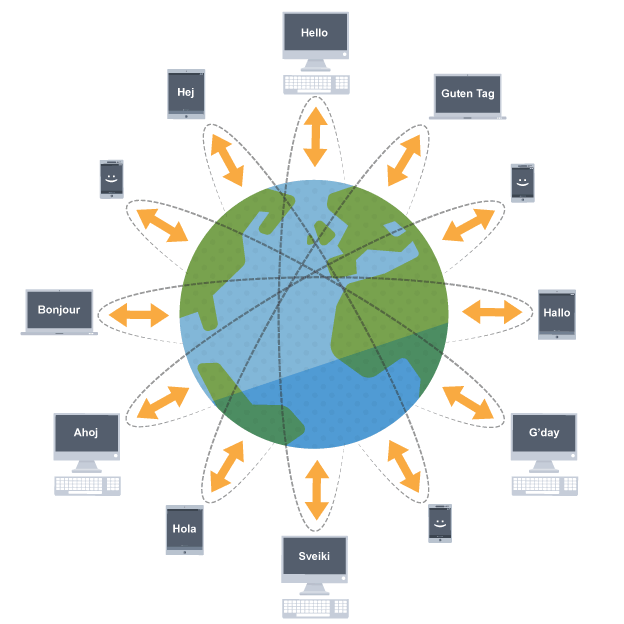
\includegraphics[width=12cm]{./net.png}
%\vspace{-10pt}
\caption{devices connected in the world}\label{wrap-fig:1}
\end{wrapfigure}

\section{\textsc{What is a network?}}

A network is two or more \emph{computers} (or other electronic devices) \textbf{connected} together, usually by cables(\textbf{guided}) or Wi-Fi(\textbf{unguided}).



\subsection{\textsc{Network benefits}}
\begin{enumerate}
\item {sharing hardware, such as printers, computers, phones, tablets, scanners, etc...}\footnotemark{}
\item {sharing software, allowing:}
    \begin{itemize}
    \item{multiple users to run the same programs on different computers}
    \item{data to be shared, so that other people can access shared work}
    \item{you to access your data from any computer on the network}
    \end{itemize}
\end{enumerate}





\footnotetext{All these pieces of hardware are usually addressed as \textbf{endpoints} as long as they have the ability to communicate effectively within a network}


\newline \noindent Networking is crucial if you want to use your computer to communicate. Without it you couldn’t send an email, a text or an instant message and that would be so weird in 2022 isn't it?

\noindent We use a huge network on a daily basis and this is called the internet. Around 5 billion\footnote{\label{peopleOnInternet}\href{https://www.oberlo.com/statistics/how-many-people-use-internet}{Oberlo statistic}.} people use the internet to share data, news and resources, amongst many other things.
\clearpage
\subsection{\textsc{guided wiring}}
Is quicker than unguided, it consists in physical wires. Optic Fiber is on the top of this list but can't be twisted or the light will bounce back. You can install an optic cable for a much longer distance and you won't get the same troubles you would get with copper cables for example. But no twisting or it'll bounce back!

\subsection{\textsc{unguided wiring}}
The term \emph{wiring} can be deceiving here as there are literally no wires involved to realize the connection. In Cantonese is probably much clearer (Figure \ref{fig:wifihk}).


\begin{wrapfigure}{R}{11cm}
\centering
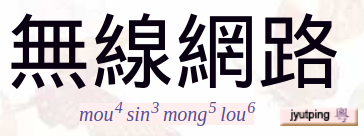
\includegraphics[width=5cm]{WiFi-HK.PNG}
%\vspace{-10pt}
\caption{Definition of WiFi in Historical Chinese commonly spoken in Hong Kong}\label{fig:wifihk}
\end{wrapfigure}


Unguided wiring simply means Wi-Fi really. You can have a 2.4Ghz signal to reach longer distance but won't be nicely matched with a 5Ghz device. A 5Ghz device won't reach the same distance as a 2.4Ghz. Take a look how it's worded in Cantonese and you'll see a different etymological meaning from the English one\footnote{\label{wifialliance}stands for Wireless Fidelity.It kept this name for a short time after the brand name was created by the \href{https://en.wikipedia.org/wiki/Wi-Fi_Alliance}{Wi-Fi Alliance}.} but still both words suggest the idea that no wires are involved.


\wrapfill


\begin{wrapfigure}{L}{8cm}
\centering\newcommand{\wrapfill}{\par\ifnum\value{WF@wrappedlines}>0
  \addtocounter{WF@wrappedlines}{-1}%
  \null\vspace{\arabic{WF@wrappedlines}\baselineskip}%
  \WFclear
\fi}
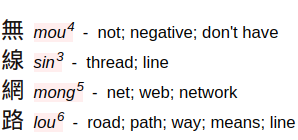
\includegraphics[width=8cm]{./WiFi-HK-details.PNG}
\vspace{-10pt}
\caption{Cantonese characters in the WiFi word}\label{wrap-fig:6}
\end{wrapfigure}


\noindent The first character represents the concept of \textbf{not} having ($mou^4$). The second one ($sin^3$) is literally thread or line so that's why \emph{wiring} to me is sort of misleading. 
If you ask a person :

\[Can\ you\ tell\ me\ what\ unguided\ wiring\ means?\]

\noindent Because of the word \emph{wiring} one could start thinking about a particular kind of special fancy wire. But wires are the last thing you'll ever see in the case of \textbf{unguided wiring}



%\begin{CJK}{UTF8}{gbsn}

%Without \texttt{CJKutf8} package, the result will be wrong.

%Café: 咖啡厅

%Gödel: 哥德尔

%© 版权所有

%無線網絡

%\end{CJK}

\section{\textsc{LAN vs WAN}}

LAN, which stands for \textbf{local area network}, and WAN, which stands for \textbf{wide area network}, are two types of networks and \texttt{\textit{as the naming conventions suggest}}, LANs are for more localized networking\footnote{\label{LAN}in a home,business,school,etc.}
\begin{wrapfigure}{R}{7cm}
\centering
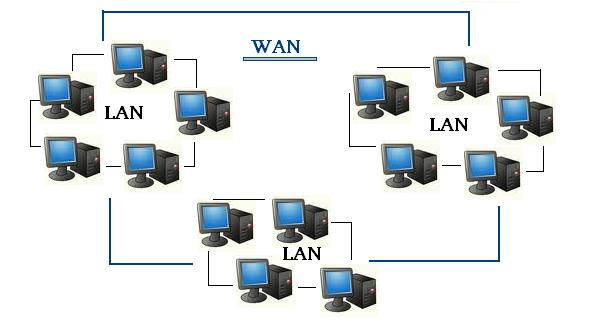
\includegraphics[width=5cm]{lan-wan.JPG}
%\vspace{-10pt}
\caption{difference between WAN and LAN}\label{wrap-fig:5}
\end{wrapfigure}

\noindent while WANs cover larger areas, such as cities, and even allow computers in different nations to connect.
LANs are typically faster and more secure than WANs, but WANs enable more widespread connectivity. Of course there are sort of exceptions like the NHS having a huge Local Area Network spread all over the country with local IP addresses starting in the first octet with \oldstylenums{10} instead of \oldstylenums{192}, thus using a Class A Address rather than a Class C (more on this topic in the Section called \textbf{The Five IPv4 Classes}) 


\chapter{Standards and Protocols}
\AddToShipoutPictureBG*{
\includegraphics[width=\paperwidth,height=\paperheight]{118.jpg}}
Here we will discuss about protocols and standards
\clearpage

\section{IEEE 802.3}

IEEE 802.3 is a set of standards and protocols that define Ethernet-based networks. Ethernet technologies
\begin{wrapfigure}[16]{1cm}
\centering
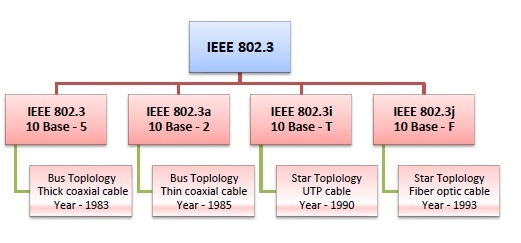
\includegraphics[width=13cm]{./ieee_802.jpg}
\vspace{-15pt}
\caption{IEEE cable hierarchy}\label{fig:ieee802}
\end{wrapfigure}

\noindent are primarily used in LANs, though they can also be used in WANs as well.

IEEE 802.3 defines the physical layer and the medium access control (MAC) sub-layer of the data link layer for wired Ethernet networks. The unique identifier of our computer's motherboard is actually adhering to a standard defined by IEEE 802.3.
The psysical layer is the lowest layer identified in the TCP/IP protocol or the ISO/OSI protocol. The packets on the network before they finally go to destination they need to know which MAC address corresponds to the IP they hold already in the headers. In the next paragraph we'll explain the different cables in Figure \ref{fig:ieee802}.




\subsection{\textsc{Popular Versions}}

There are a number of versions of IEEE 802.3 protocol. The most popular ones are:

\begin{itemize}
\item{IEEE 802.3: This was the original standard given for coaxial (10BASE-5). Here, 10 is the maximum throughput which means 10 Mbps and 5 refers to the maximum segment length of 500m. If it goes longer than 500m there's no guarantee it'll work}
\item{IEEE 802.3a: This gave the standard for thin coax (10BASE-2), which is a thinner variety of coaxial cable. The 2 refers to the maximum segment length of about 200m (185m to be precise)}
\item{IEEE 802.3j: This gave the standard for Ethernet over Fiber (10BASE-F) that uses fiber optic cables as medium of transmission}
\end{itemize}

\clearpage

\section{\textsc{Protocols}}

Protocols are kind of rules defined in advance to make sure two or more devices know in advance what to expect if they send a particular message and what to expect in return 

\subsection{\textsc{OSI Standard}}
The Open Systems Interconnection (OSI) model describes seven layers that computer systems use to communicate over a network. It was the first standard model for network communications, adopted by all major computer and telecommunication companies. %in the early 1980s

\begin{wrapfigure}[21]{5cm}
\centering
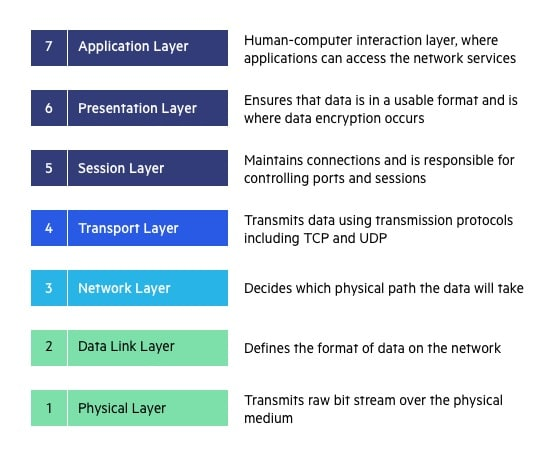
\includegraphics[width=12cm]{./OSI-7-layers.jpg}
%\vspace{-10pt}
\caption{OSI Layer representation}\label{fig:osilayers}
\end{wrapfigure}


The modern Internet is not based on OSI, but on the simpler TCP/IP model. However, the OSI 7-layer model is still widely used, as it helps visualize and communicate how networks operate, and helps isolate and troubleshoot networking problems.


\subsection{\textsc{A good Mnemonic}}
One way to remember the OSI Layer is, as always, by using funny and silly stories but this time we won't be talking of italian clichés, mentioning videogames monsters or referencing Boris Johnson jumping from an airplane holding the British Flag (yes he did that as well) but we'll use this mnemonic insetead: 

\medskip
\noindent
\textsc{\textbf{P}lease \textbf{D}o \textbf{N}ot \textbf{T}hrow \textbf{S}ausage and \textbf{P}izza Away}}
\medskip

\noindent It's obtained by looking at the $1^{st}$ letter of each layer from the bottom

\subsection{\textsc{Theory vs Practice}}
Even if The Transmission Control Protocol/Internet Protocol (TCP/IP) model came before the Open Systems Interconnection (OSI) model it is what is used in practice today, and it has only five layers:

\begin{itemize}
\item {Application layer}
\item {Transport layer}
\item {Network access layer}
\item {Network interface layer}
\item {Hardware layer}
\end{itemize}

\noindent It may look different from the OSI model, but some functions are just encompassed in a single layer which is  \textbf{the application layer} corresponding to $Application^{OSI}$,$Presentation^{OSI}$ and $Session^{OSI}$.

\subsubsection{\textsc{connection-oriented protocols}}
Unlike UDP, TCP/IP is a \textbf{connection-oriented} protocol\footnote{\label{tcpsocket}James F. Kurose and Keith W. Ross \href{https://gaia.cs.umass.edu/kurose_ross/online_lectures.htm}{Computer Networking A Top-Down Approach}.}}. This means that before the client and server can start to send data to each other, they first need to \textbg{handshake} and establish a TCP connection. One end of the TCP connection is attached to the client socket and the other end is attached to a server socket. When creating the TCP connection, we associate it with the client socket address(IP address and port number). With the TCP connection established, when one side wants to send data to the other side, it just drops the data into the TCP connection via its socket. This is different from UDP, for which the server must attach a destination address to the packet before dropping it into the socket.

Now let’s take a closer look at the interaction of client and server programs in TCP. The client has the job of initiating contact with the server. In order for the server to be able to react to the client’s initial contact, the server has to be ready. This implies two things. First, as in the case of UDP, the TCP server must be running as a process before the client attempts to initiate contact. Second, the server program must have a special door, more precisely a special socket, that welcomes some initial contact from a client process running on an arbitrary host. Using our \textbf{house/door} analogy for a \textbf{process/socket}, we will sometimes refer to the client’s initial contact as “knocking on the welcoming door.”

With the server process running, the client process can initiate a TCP connection to the server. This is done in the client program by creating a TCP socket. When the client creates its TCP socket, it specifies the address of the welcoming socket in the server, namely, the IP address of the server host and the port number of the socket. After creating its socket, the client initiates a \textbf{three-way handshake} and establishes a
TCP connection with the server. The three-way handshake, which takes place within the transport layer, is completely invisible to the client and server programs.

\begin{wrapfigure}{4cm}
\centering
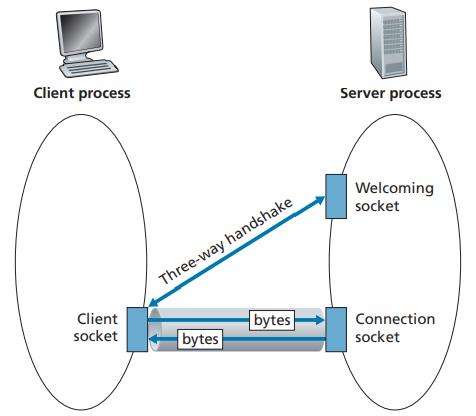
\includegraphics[width=7.4cm]{./tcp-socket.PNG}
%\vspace{-10pt}
\caption{The TCPServer process has two sockets}\label{fig:tcpsocket}
\end{wrapfigure}

During the three-way handshake, the client process knocks on the welcoming door of the server process. When the server “hears” the knocking, it creates a new door, more precisely, a new socket that is dedicated to that particular client. In our example below, the welcoming door is a TCP socket object that we call serverSocket; the newly created socket dedicated to the client making the connection is called connectionSocket. People encountering TCP sockets for the first time sometimes confuse the welcoming socket (which is the initial
point of contact for all clients wanting to communicate with the server), and each newly created server-side connection socket that is subsequently created for communicating with each client.

From the application’s perspective, the client’s socket and the server’s connection socket are directly connected by a pipe. As shown in Figure \ref{fig:tcpsocket}, the client process can send arbitrary bytes into its socket, and TCP guarantees that the server process will receive (through the connection socket) each byte in the order sent. TCP thus provides a reliable service between the client and server processes.
Furthermore, just as people can go in and out the same door, the client process not only sends bytes into but also receives bytes from its socket; similarly, the server process not only receives bytes from but also sends bytes into its connection socket.

\subsubsection{\textsc{connectionless protocols}}

UDP is a no-frills, lightweight transport protocol, providing minimal services. UDP is connectionless, so there is no handshaking before the two processes start to communicate. UDP provides an unreliable data transfer service, which means, when a process sends a message into a UDP socket, UDP provides no guarantee that the message will ever reach the receiving process. Furthermore, messages that do arrive at the
receiving process may arrive out of order.

UDP does not include a congestion-control mechanism, so the sending side of UDP can pump data into the layer below (the network layer) at any rate it pleases. (Note, however, that the actual end-to-end throughput may be less than this rate due to the limited transmission capacity of intervening links or due to congestion).


\subsubsection{\textsc{horizontal vs vertical approach}}

\epigraph{In the OSI model,the layers communicate directly with each other, hence horizontal approch.

While in TCP/IP, each layer is traversed meaning data travels each layer, only then it is sent, hence vertical approch.}{\textit{horizontal and vertical approaches \\Quora.com}}

\noindent If someone can explain to me how to interpret the message Quora.com is trying to convey or in general which protocol is horizontal and which is vertical and most importantly what's horizontal and vertical definition, then I'd be all ears and ready to learn but until then it'll be a mistery that someone one day will solve \textbf{but that day is not today and it won't be me}. If a question like this comes out in the exam I'll just have a random guess

%\medskip
%\begin{displayquote}
%In the OSI model, there are no intermediate nodes between transport layer or above layers, hence these layers communicate directly with each other, hence horizontal approch.
%While in TCP/IP, each layer is traversed starting from application layer to transport layer then internet layer then goes to the host and then the network layer, and then msg is sent. Meaning data travels each layer, accessing their functionality, only then it is sent, hence vertical approch.
%\end{displayquote}
%\medskip

\clearpage

\section{Switched Local Area Networks}

\begin{wrapfigure}[15]{R}{9cm}
\centering
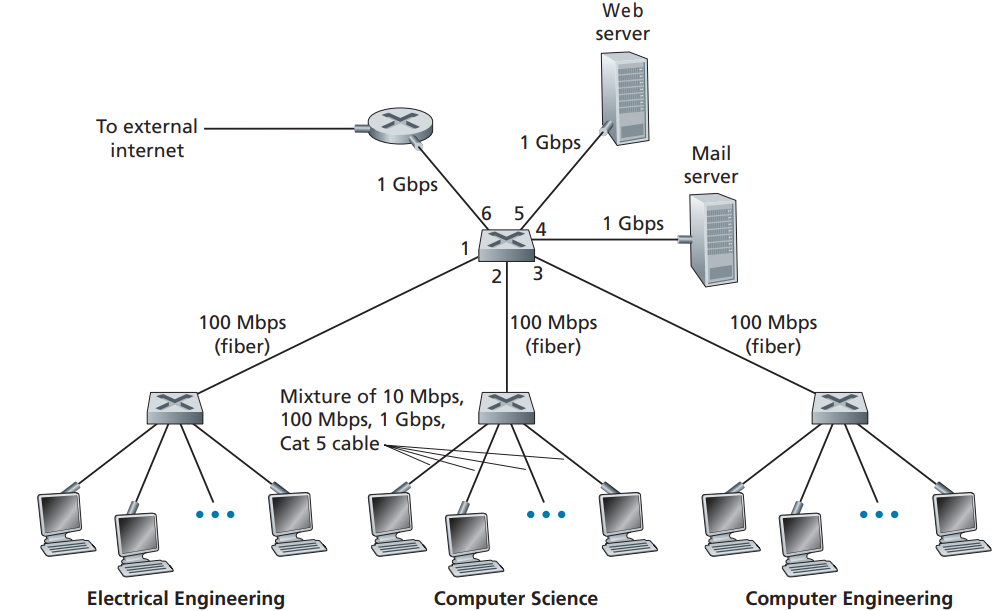
\includegraphics[width=9.5cm]{./switched-lan.PNG}
%\vspace{-10pt}
\caption{An institutional network connected together by four switches}\label{fig:switched-lan}
\end{wrapfigure}


Let's do now talk about Switched local networks.

Figure \ref{fig:switched-lan} shows a switched local network connecting two servers, three departments and a router using four switches. Since these switches operate at the link layer (layer-2 if you recall Figure \ref{fig:osilayers}), they switch link-layer frames (instead of network-layer datagrams\footnote{\label{datagram}basic transfer unit associated with a packet-switched network structured in header and payload providing connectionless communication service}), hence don’t recognize network-layer addresses, thus don’t use routing algorithms like for example OSPF to determine paths through the network of layer-2 switches. Rather than using IP addresses, we will soon see that they use link-layer addresses to forward link-layer frames through the network of switches. We shall approach switched LANs by first covering linklayer addressing (Section \ref{section:link-layer}). We then take a close look to the famous Ethernet protocol (Section -.-.-). Once we've seen the link-layer addressing and Ethernet, we’ll look at how link-layer switches operate (Section -.-.-), and then see (Section -.-.-) how these switches are often used to build large-scale LANs.


\subsection{Link-layer addressing and ARP}
\label{section:link-layer}

Hosts and routers have link-layer addresses. You might be asking, why in the world do we need to have addresses at both the network and link layers? In addition to describing the syntax and function of the link-layer addresses, in this section we hope to shed some light on why the two layers of addresses are useful and, in fact, indispensable. We’ll also cover the Address Resolution Protocol (ARP), which provides a mechanism to translate IP addresses to link-layer addresses.

\subsubsection{MAC Addresses}
The truth is, hosts and routers don't have link-layer addresses but their adapters (their network interfaces) do instead. A host or router with multiple network interfaces will thus have multiple link-layer addresses associated with it, just as it would also have multiple IP addresses associated with it.

\wrapfill
\begin{wrapfigure}{L}{8cm}
\centering\newcommand{\wrapfill}{\par\ifnum\value{WF@wrappedlines}>0
  \addtocounter{WF@wrappedlines}{-1}%
  \null\vspace{\arabic{WF@wrappedlines}\baselineskip}%
  \WFclear
\fi}
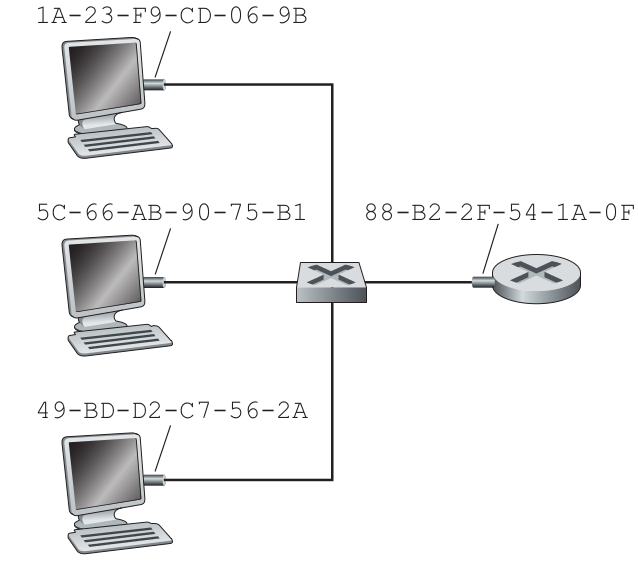
\includegraphics[width=4cm]{./addressless-switch.PNG}
\vspace{-10pt}
\caption{Each interface connected to a LAN has a unique MAC address}\label{fig:addressless-switch}
\end{wrapfigure}


\noindent It’s important to note, however, that link-layer switches do not have link-layer addresses associated with their interfaces that connect to hosts and routers.This is because the job of the link-layer switch is to carry datagrams between hosts and routers; a switch does this job transparently, that is, without the host or router having to explicitly address the frame to the intervening switch. This is illustrated in Figure \ref{fig:addressless-switch}. A linklayer address is variously called a \textbf{LAN address}, a \textbf{physical address}, or a \textbf{MAC address}. Because MAC address seems to be the most popular term, we’ll henceforth refer to link-layer addresses as MAC addresses. For most LANs (including Ethernet and 802.11 wireless LANs), the MAC address is 6 bytes long, giving $2^{48}$ possible MAC addresses. As shown in Figure \ref{fig:addressless-switch}, these 6-byte addresses are typically expressed in HEX notation. Although MAC addresses were designed to be permanent, it is now possible to change an adapter’s MAC address via software. For the rest of this section, however, we’ll assume that an adapter’s MAC address is fixed.

One MAC address is unique in the world altough adapters are manufactured in many countries by many companies. How does a company manufacturing adapters in Liechtenstein make sure that it is using different addresses from a company manufacturing adapters in Singapore? IEEE manages the MAC address space. In particular, when a company wants to manufacture adapters, it purchases a chunk of the address space consisting of $2^{24}$ addresses for a nominal fee. IEEE allocates the chunk of $2^{24}$ addresses by fixing the first 24 bits of a MAC address and letting the company create unique combinations of the last 24 bits for each adapter.

An adapter’s MAC address has a flat structure (as opposed to a hierarchical structure) and doesn’t change no matter where the adapter goes. A laptop with an Ethernet interface always has the same MAC address, no matter where the computer goes. A smartphone with an 802.11 interface always has the same MAC address, no matter where the smartphone goes. Recall that, in contrast, IP addresses have a hierarchical structure (that is, a network part and a host part), and a host’s IP addresse needs to be changed when the host moves,for example the host is attached to another network. An adapter’s MAC address is analogous to a person’s National Insurance Number, which also has a flat addressing structure and which doesn’t change no matter
where the person goes. An IP address is analogous to a person’s postal address, which is hierarchical and which must be changed whenever a person moves. Just as a person may find it useful to have both a postal address and a NIN, it is useful for a host and router interfaces to have both a network-layer address (IP) and
a MAC address.

When an adapter wants to send a frame to some destination adapter, the sending adapter inserts the destination adapter’s MAC address into the frame and then sends the frame into the LAN. As we will soon see (TO-DO), a switch occasionally broadcasts an incoming frame onto all of its interfaces. We’ll see in Chapter - that 802.11 also broadcasts frames. Thus, an adapter may receive a frame that isn’t addressed to it. Thus, when
an adapter receives a frame, it will check to see whether the destination MAC address in the frame matches its own MAC address. If there is a match, the adapter extracts the enclosed datagram and passes the datagram up the protocol stack. If there isn’t a match, the adapter discards the frame, without passing the network-layer datagram up. Thus, only the destination adapter will be interrupted when the frame is received.

However, sometimes a sending adapter \emph{does} want all the other adapters on the LAN to receive and process the frame it is about to send. In this case, the sending adapter inserts a special MAC \textbf{broadcast address} into the destination address field of the frame. For LANs that use 6-byte addresses (such as Ethernet and 802.11), the broadcast address is a string of 48 consecutive 1s (that is, FF-FF-FF-FF-FF-FF in hexadecimal notation).


\subsubsection{Address Resolution Protocol (ARP)}

Because there are both network-layer addresses (for example, Internet IP addresses) and link-layer addresses (that is, MAC addresses), there is a need to translate between them. For the Internet, this is the job of the Address Resolution Protocol (ARP). To understand the need for a protocol such as ARP, consider the network shown in Figure \ref{fig:ARP}. In this simple example, each host and router has a single IP address and single MAC address. As usual, IP addresses are shown in dotted-decimal

\begin{wrapfigure}{R}{9cm}
\centering
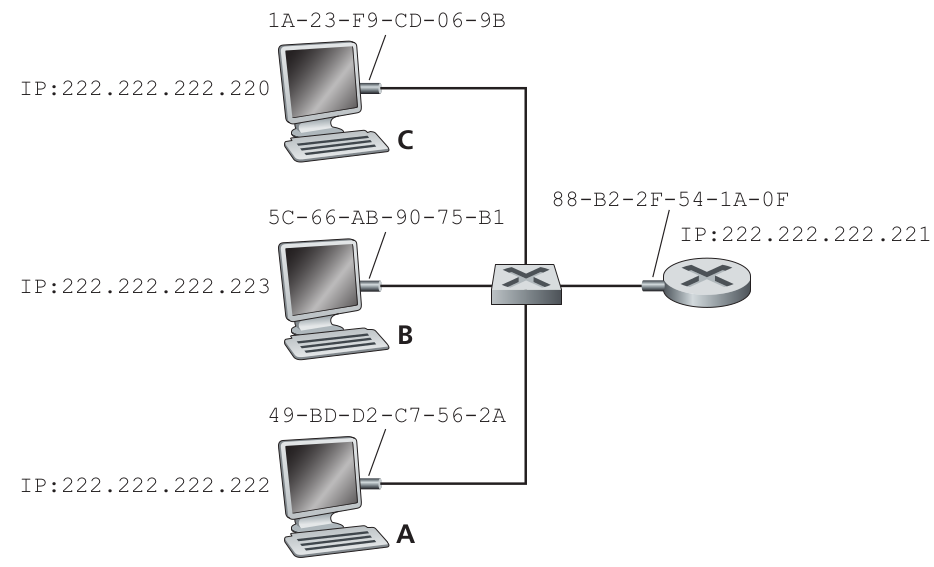
\includegraphics[width=9.5cm]{./ARP.PNG}
%\vspace{-10pt}
\caption{Each interface on a LAN has an IP address and a MAC address}\label{fig:ARP}
\end{wrapfigure}

notation and MAC addresses are shown in hexadecimal notation. For the purposes of this discussion, we will assume in this section that the switch broadcasts all frames, which means, whenever a switch receives a frame on \emph{one interface}, it forwards the frame on all of its \emph{other interfaces}. In the next section(?), we will provide a more accurate explanation of how switches operate.

Now suppose that the host with IP address 222.222.222.220 wants to send an IP datagram to host 222.222.222.222. In this example, both the source and destination are in the same subnet. To send a datagram, the source must give its adapter not only the IP datagram but also the MAC address for destination 222.222.222.222. The sending adapter will then construct a link-layer frame containing the destination’s MAC address and send the frame into the LAN.

The important question addressed in this section is, How does the sending host determine the MAC address for the destination host with IP address 222.222.222.222? It uses ARP. An ARP module in the sending host takes any IP address on the same LAN as input, and returns the corresponding MAC address. In the example at hand, sending host 222.222.222.220 provides its ARP module the IP address 222.222.222.222, and the ARP module returns the corresponding MAC address 49-BD-D2-C7-56-2A. So we see that ARP resolves an IP address to a MAC address. In many ways it is analogous to DNS, which resolves host names to IP addresses. However, one important difference between the two resolvers is that DNS resolves host names for hosts anywhere in the Internet, whereas ARP resolves IP addresses only for hosts and router interfaces on the same subnet. If a node in California were to try to use ARP to resolve the IP address for a node in Mississippi, ARP would return with an error.

Now that we have explained what ARP does, let’s look at how it works. Each host and router has an ARP table in its memory, which contains mappings of IP addresses to MAC addresses.

Figure \ref{fig:ARP-table} shows what an ARP table in host 222.222.222.220 might look like.

\begin{wrapfigure}{R}{9cm}
\centering
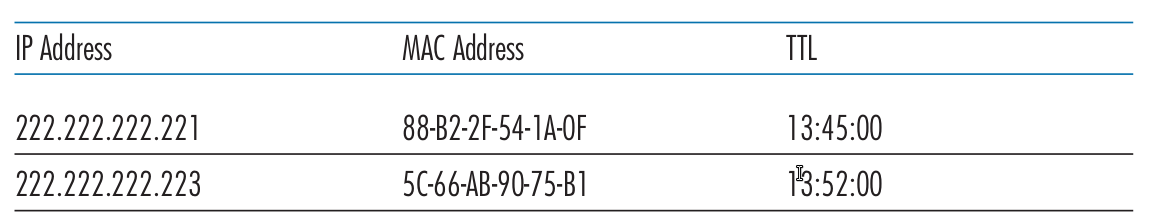
\includegraphics[width=9.5cm]{./ARP-table.PNG}
%\vspace{-10pt}
\caption{A possible ARP table in 222.222.222.220}\label{fig:ARP-table}
\end{wrapfigure}

The ARP table also contains a time-to-live (TTL) value, which indicates when each mapping will be deleted from the table. Note that a table does not necessarily contain an entry for every host and router on the subnet; some may have never been entered into the table, and others may have expired. A typical expiration time for an entry is 20 minutes from when an entry is placed in an ARP table.

Now suppose that host 222.222.222.220 wants to send a datagram that is IP-addressed to another host or router on that subnet. The sending host needs to obtain the MAC address of the destination given the IP address. This task is easy if the sender’s ARP table has an entry for the destination node. But what if the ARP table doesn’t cur-
rently have an entry for the destination? In particular, suppose 222.222.222.220 wants to send a datagram to 222.222.222.222. In this case, the sender uses the ARP protocol to resolve the address. First, the sender constructs a special packet called an ARP packet. An ARP packet has several fields, including the sending and receiving IP and MAC addresses. Both ARP query and response packets have the same format. The pur-
pose of the ARP query packet is to query all the other hosts and routers on the subnet
to determine the MAC address corresponding to the IP address that is being resolved.

Returning to our example, 222.222.222.220 passes an ARP query packet to the adapter along with an indication that the adapter should send the packet to the MAC broadcast address, namely, FF-FF-FF-FF-FF-FF. The adapter encapsulates the ARP packet in a link-layer frame, uses the broadcast address for the frame’s destination address, and transmits the frame into the subnet. Recalling our NIN/postal address analogy, an ARP query is equivalent to a person shouting out with a loudhailer in a small street in Walthamstow Central “What is the NIN of the person whose postal address is \textbf{35, Folkestone road E17 9SD}?” The frame containing the ARP query is received by all the other adapters on the subnet, and (because of the broadcast address) each adapter
passes the ARP packet within the frame up to its ARP module. Each of these ARP modules checks to see if its IP address matches the destination IP address in the ARP packet. The one with a match sends back to the querying host a response ARP packet with the desired mapping. The querying host 222.222.222.220 can then update its
ARP table and send its IP datagram, encapsulated in a link-layer frame whose destination MAC is that of the host or router responding to the earlier ARP query.

\paragraph{[arp -a] output on my linux shell}
\begin{flushleft}
On my machine for example the ARP table contains just two entries, one for the gateway, and one for the TV who's connected in the same WiFi. The LAN is obviously larger than that but my computer never had the need to send other machines a packet.
\end{flushleft}

\begin{lstlisting}
_gateway (192.168.0.1) at 24:a7:dc:31:5b:d1 [ether] on wlp3s0
TV (192.168.0.129) at cc:d3:c1:64:f9:f3 [ether] on wlp3s0
\end{lstlisting}

\subsubsection{RARP and DHCP}
RARP demands another computer (usually a server in the same LAN) to assign the demanding one with an IP which is essentially what DHCP is doing that's why RARP got obsolete

\clearpage

\section{Networking Hardware}
Computers need networking hardware in order to connect to each other. \textbf{Routers}, \textbf{hubs}, \textbf{switches} and \textbf{bridges} are all pieces of networking equipment that can perform slightly different tasks. A router can often incorporate hubs, switches and wireless access within the same hardware

\begin{wrapfigure}[18]{3cm}
\centering
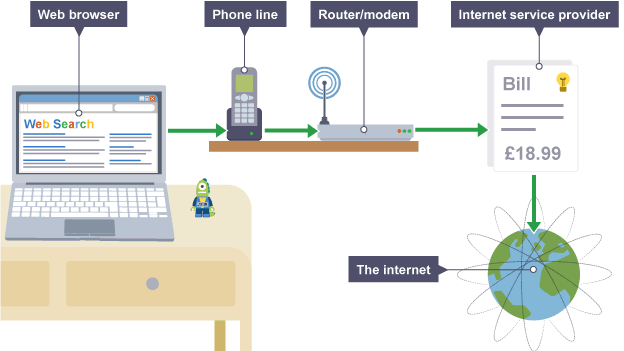
\includegraphics[width=14cm]{./large.PNG}
%\vspace{-10pt}
\caption{Router connecting devices in a LAN over the Internet}\label{wrap-fig:4}
\end{wrapfigure}

\subsection{Routers}
A router can form a \textbf{LAN} by connecting devices within a building. It also makes it possible to connect different networks together. Homes and businesses use a router to connect to the internet. A router can often incorporate a modem within the hardware.

\subsection{Modems}
A \textbf{modem} enables a computer to connect to the internet over a telephone line. A modem converts \textbf{digital} signals from a computer to analogue signals that are then sent down the telephone line. A modem on the other end converts the analogue signal back to a digital signal which another computer can understand.

\subsection{Hubs, bridges and switches}
\textbf{Hubs}, \textbf{bridges} and \textbf{switches} allow multiple devices to connect to the router and they transfer data to all devices on a network. A router is a more complex device that usually includes the capability of hubs, bridges and switches.

\clearpage

\subsubsection{Hubs}

\begin{wrapfigure}[21]{R}{11cm}
\centering
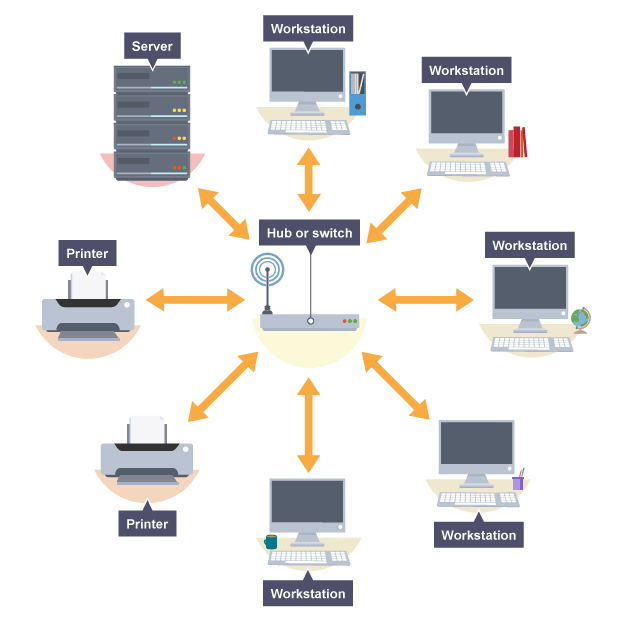
\includegraphics[width=10cm]{./hbs.PNG}
%\vspace{-10pt}
\caption{devices connected together}\label{wrap-fig:5}
\end{wrapfigure}

A hub broadcasts data to all devices on a network. This can use a lot of \textbf{bandwidth} as it results in unnecessary data being sent - not all computers might need to receive the data. A hub would be useful to link up a few games consoles for a local multiplayer game using a wired LAN.
A hub is a physical-layer device that acts on individual bits rather than frames.When a bit, representing a zero or a one, arrives from one interface, the hub simply re-creates the bit, boosts its energy strength, and transmits the bit onto all the other interfaces. Thus, Ethernet with a hub-based star topology is also a broadcast LAN.

Whenever a hub receives a bit from one of its interfaces, it sends a copy out on all of its other interfaces. In particular, if a hub receives frames from two different interfaces at the same time, a collision occurs and the nodes that created the frames must retransmit.At some point many hubs got replaced with switches which are “collision-less” but unlike routers, which operate up through layer 3, switches operates only up through layer 2.


\wrapfill


\begin{wrapfigure}{L}{8cm}
\centering\newcommand{\wrapfill}{\par\ifnum\value{WF@wrappedlines}>0
  \addtocounter{WF@wrappedlines}{-1}%
  \null\vspace{\arabic{WF@wrappedlines}\baselineskip}%
  \WFclear
\fi}
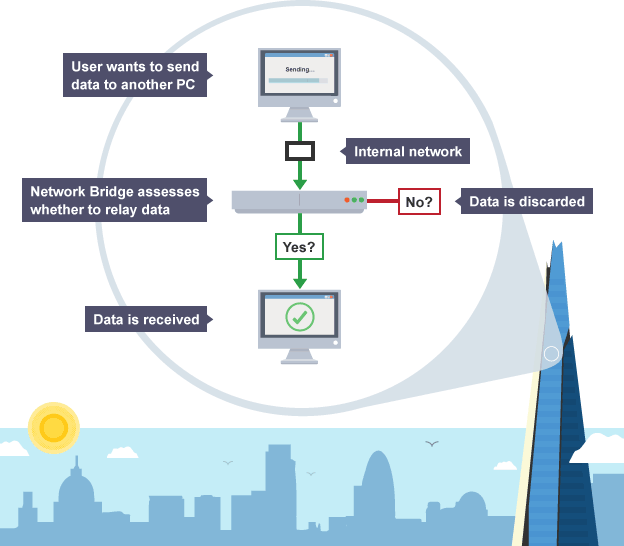
\includegraphics[width=8cm]{./performance.PNG}
\vspace{-10pt}
\caption{Bridge saving unnecessary data transfer}\label{fig:bridge}
\end{wrapfigure}


\subsubsection{Bridges}
A \textbf{bridge} is used to connect two separate LAN networks. A computer can act as a bridge through the \textbf{operating system}. A bridge looks for the receiving device before it sends the message. This means that it will not send a message if the receiving computer is not there. It will check to see if the receiver has already had the message. This can help save unnecessary data transfers, which improves the performance of a network.(see Figure \ref{fig:bridge})

\wrapfill
\clearpage

\subsubsection{Switches}
A \textbf{switch} performs a similar role to a hub and a bridge but is more powerful. It stores the \textbf{MAC addresses} of devices on a network and filters \textbf{data packets} to see which devices have asked for them. This makes a switch more efficient when demand is high. If, for example, a game involved lots of data being passed between machines, then a switch could reduce the amount of \textbf{latency}

\section{Cisco Packet Tracer}

Packet Tracer is a cross-platform visual simulation tool designed by Cisco Systems that allows users to create network topologies and imitate modern computer networks. The software allows users to simulate the configuration of Cisco routers and switches using a simulated command line interface. Packet Tracer makes use of a drag and drop user interface, allowing users to add and remove simulated network devices as they see fit. The software is mainly focused towards Cisco Networking Academy students as an educational tool for helping them learn fundamental CCNA concepts. Previously students enrolled in a CCNA Academy program could freely download and use the tool free of charge for educational use.\footnotemark{} \newline

In this experiment we try to ping devices being set with 0 in the IP fields. Then we're gonna expand the network with more devices

\footnotetext{Bakni, Michel; Cardinale, Yudith; Moreno, Luis Manuel (June 2018). \textbf{An Approach to Evaluate Network Simulators: An Experience with Packet Tracer}.Revista Venezolana de Computación. 5: 29–36. ISSN 2244-7040. \newline Javid,Sheikh Raashid (May 2014). \textbf{Role of Packet Tracer in learning Computer Networks} (PDF). International Journal of Advanced Research in Computer and Communication Engineering. 3 (5): 6508–6511.}

\begin{itemize}
\item{First nextwork has a 192.168.1.1 default gateway}
\item{Second network has a 192.168.0.1 default gateway}
\end{itemize}

\clearpage

\subsection{The step-by-step guide}

\href{https://monsterhunter.fandom.com/wiki/Seregios}{Seregios}\footnote{\label{seregios}Seregios is a Flying Wyvern introduced in \href{https://monsterhunter.fandom.com/wiki/Monster_Hunter_4_Ultimate}{Monster Hunter 4 Ultimate}.} wants to create a network on Cisco Packet Tracer. The task is quite easy but he's got quite a few tasks to accomplish

\begin{wrapfigure}{3cm}
\centering
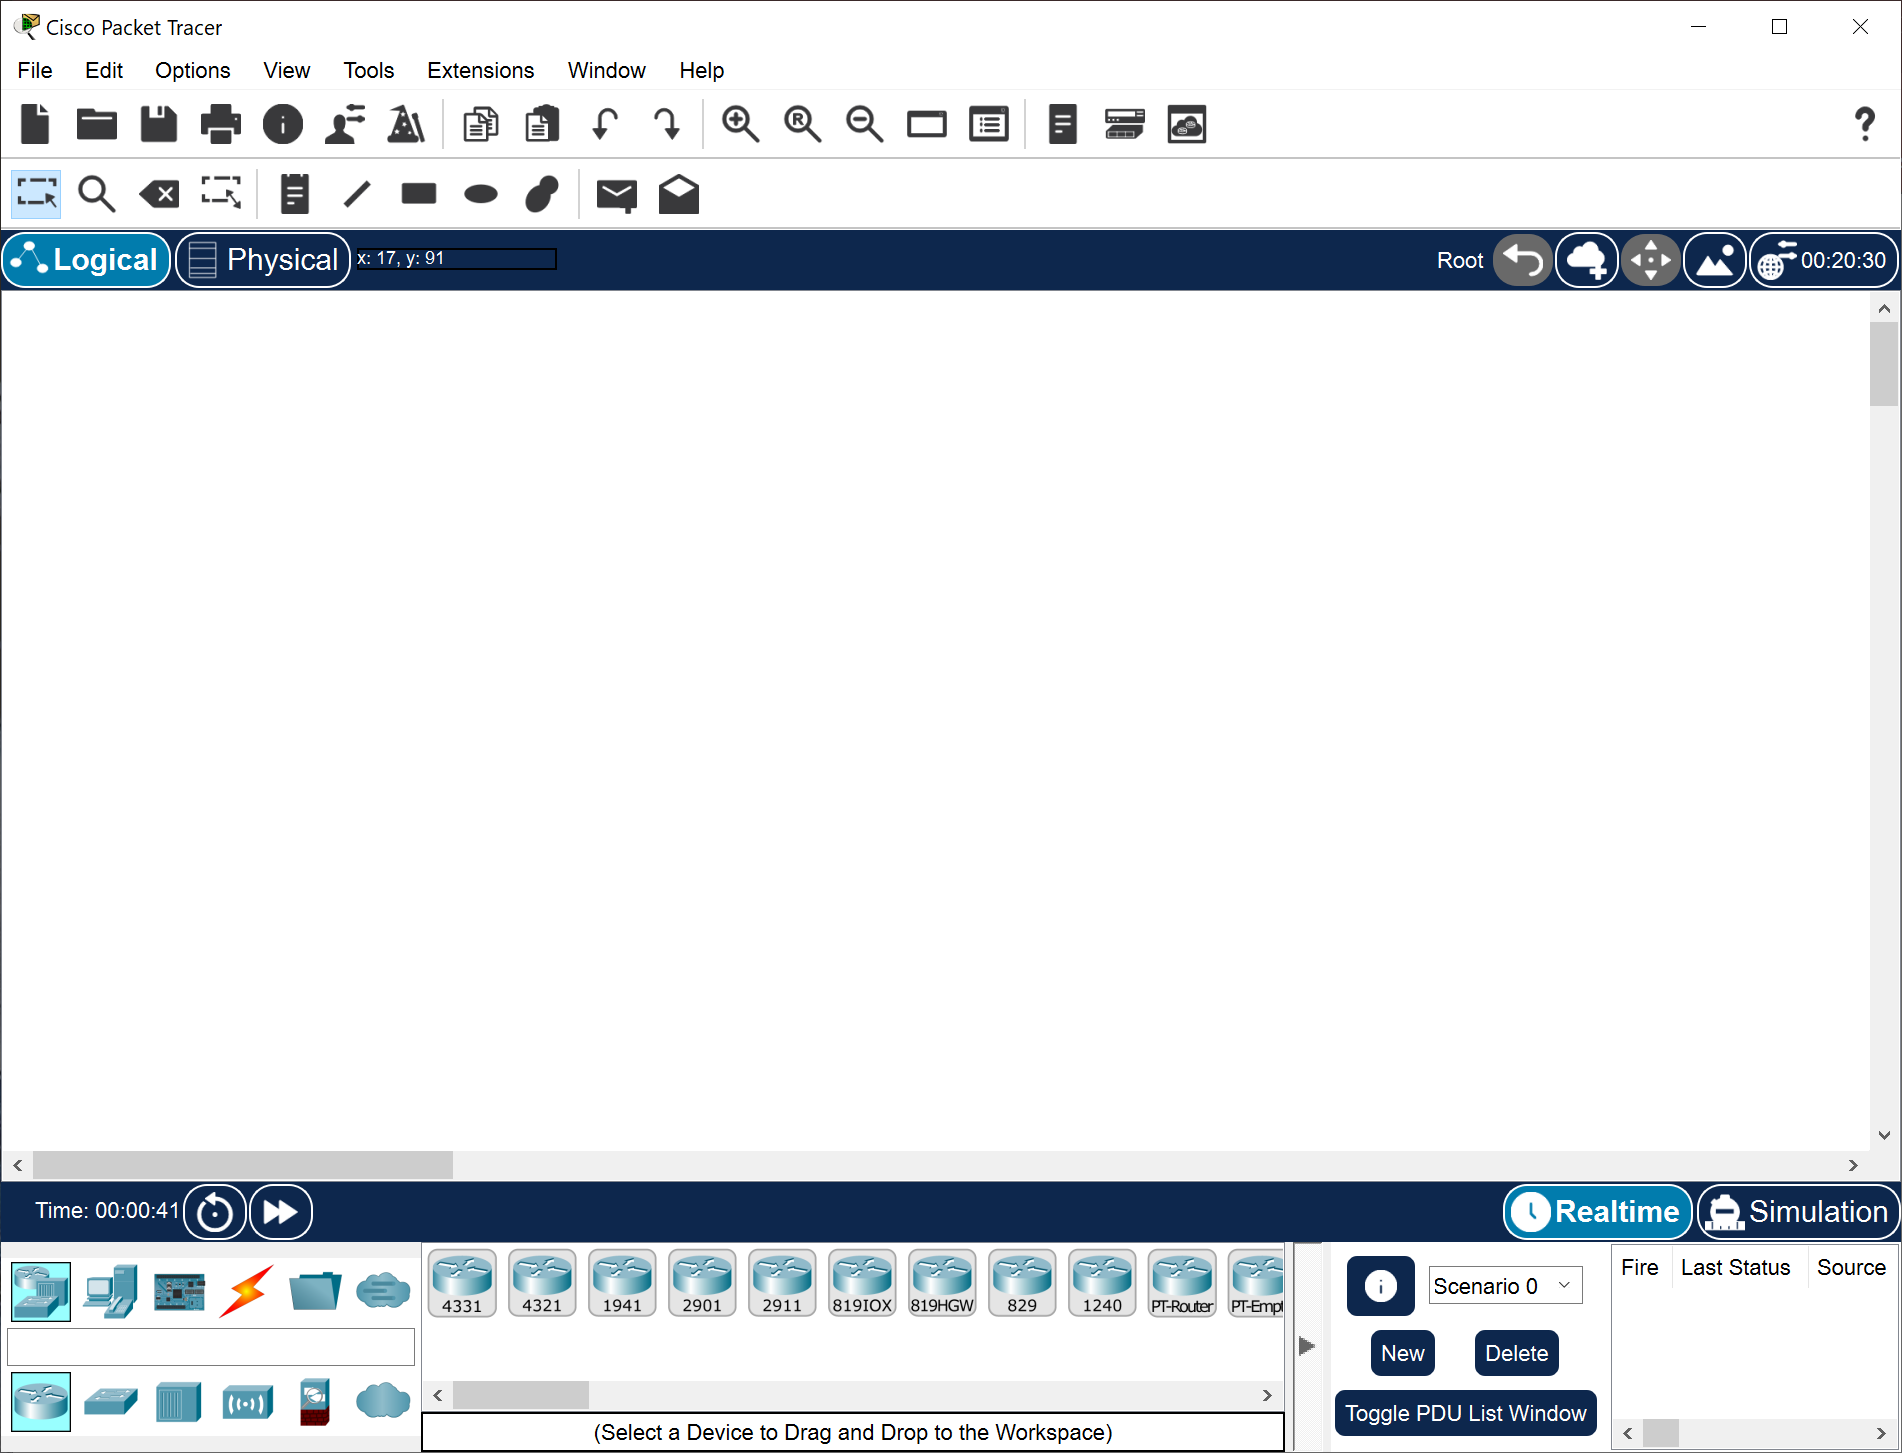
\includegraphics[width=13cm]{./step-by-step/0.PNG}
%\vspace{-10pt}
\caption{first screen he gets when he opens Cisco Packet Tracer}\label{wrap-fig:100}
\end{wrapfigure}

The first he needs to do is opening Cisco Packet Tracer. The screen will be completely empty with no devices selected. On the right hand side of the bottom panel \textbf{Realtime} is being selected instead of \textbf{Simulation} \newline

\clearpage

\noindent Now what he needs to do is to add a switch : \newline

\noindent 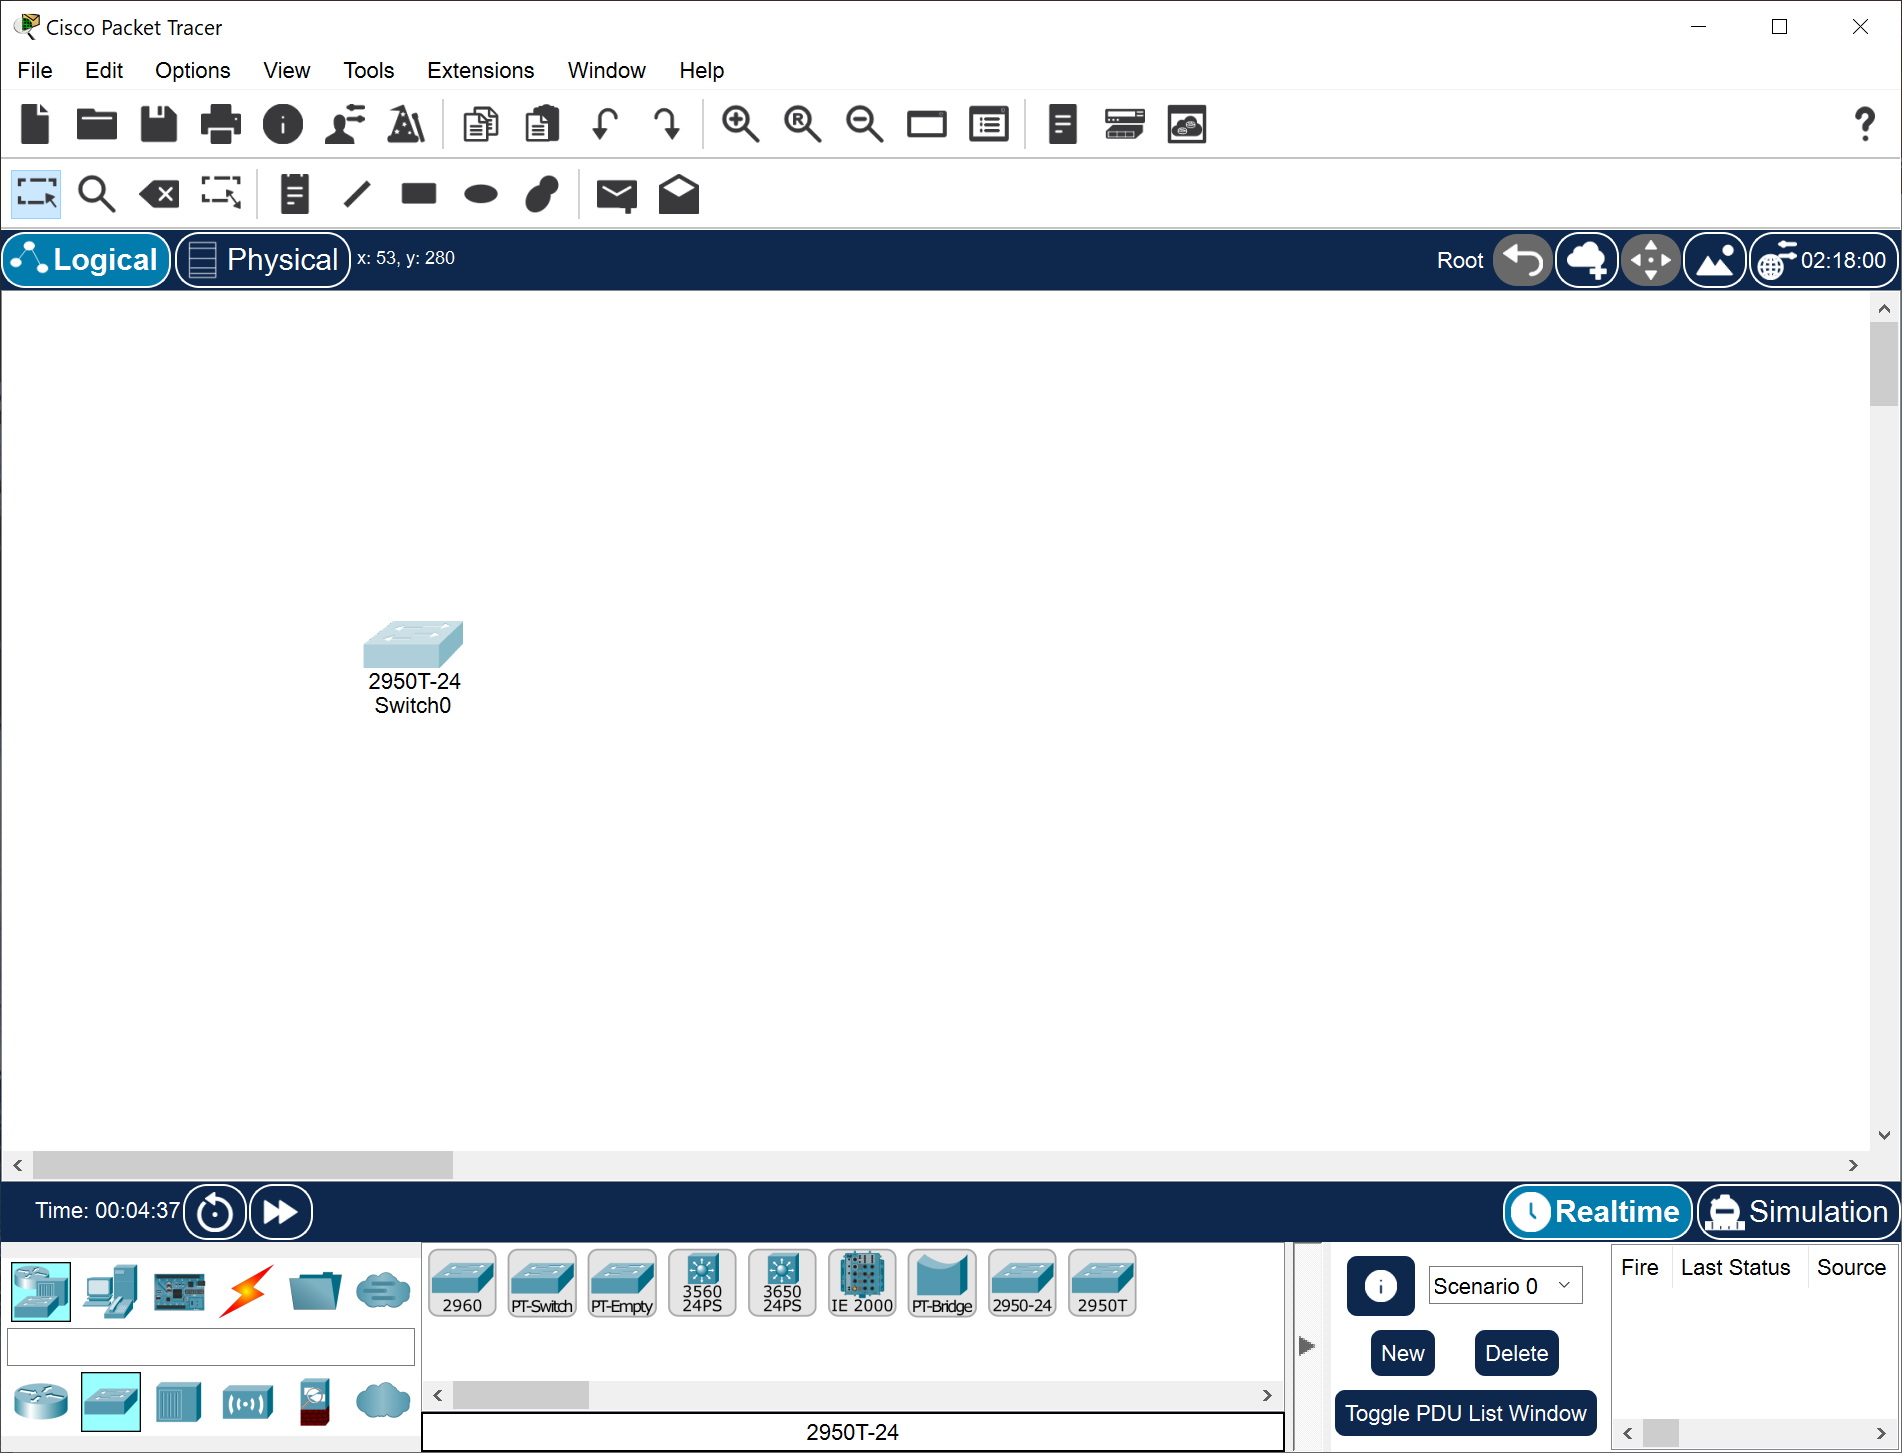
\includegraphics[width=13cm]{./step-by-step/1.PNG}
\clearpage

\noindent And then we add a computer : \newline

\noindent 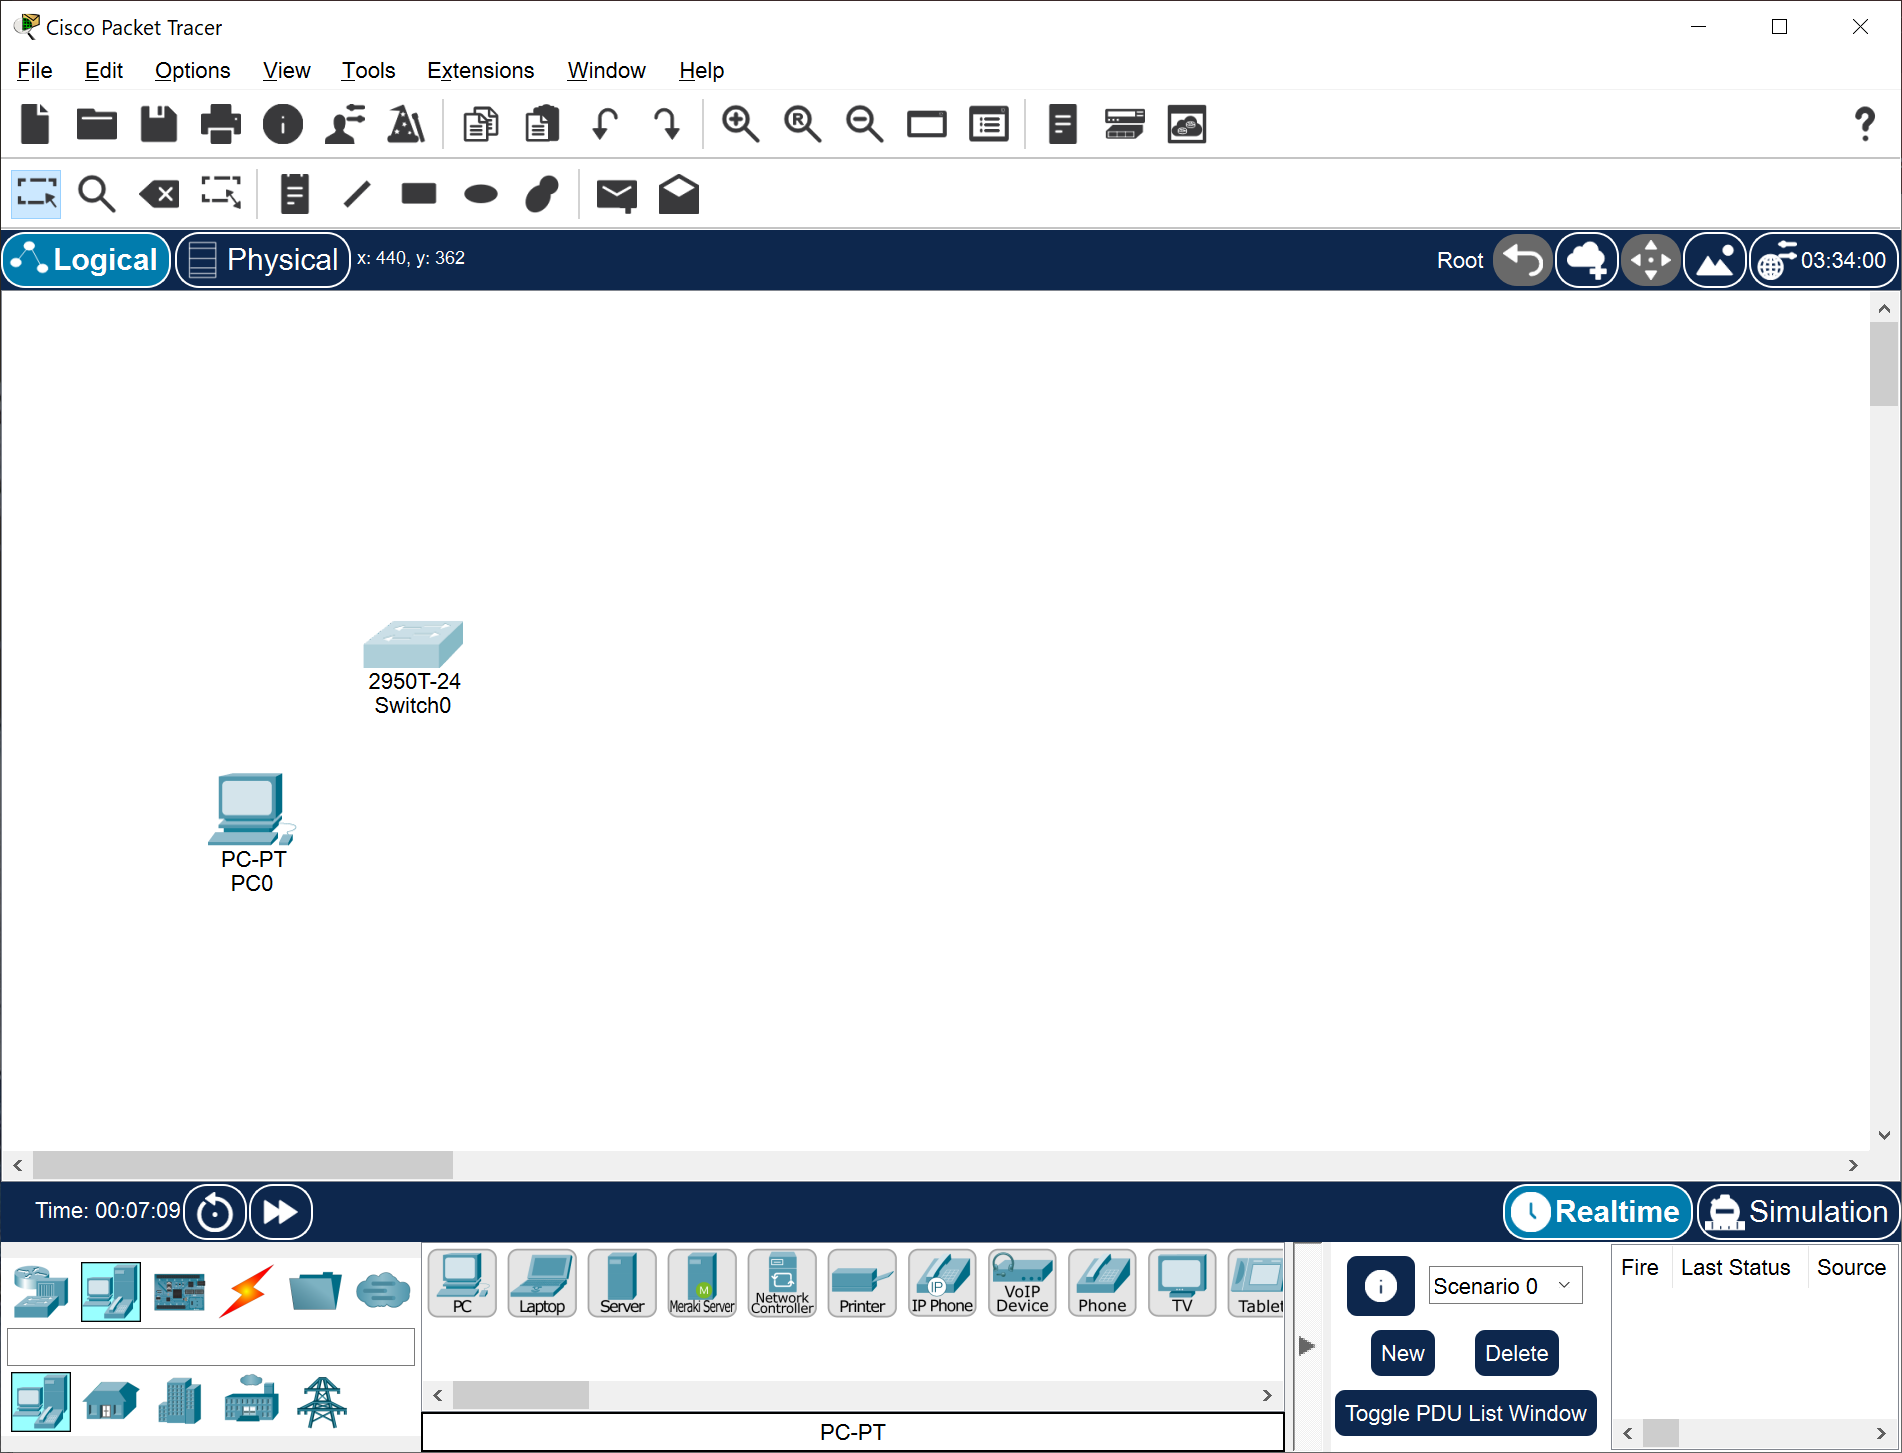
\includegraphics[width=13cm]{./step-by-step/2.PNG}
\clearpage

\noindent Now we click on the computer \newline

\noindent 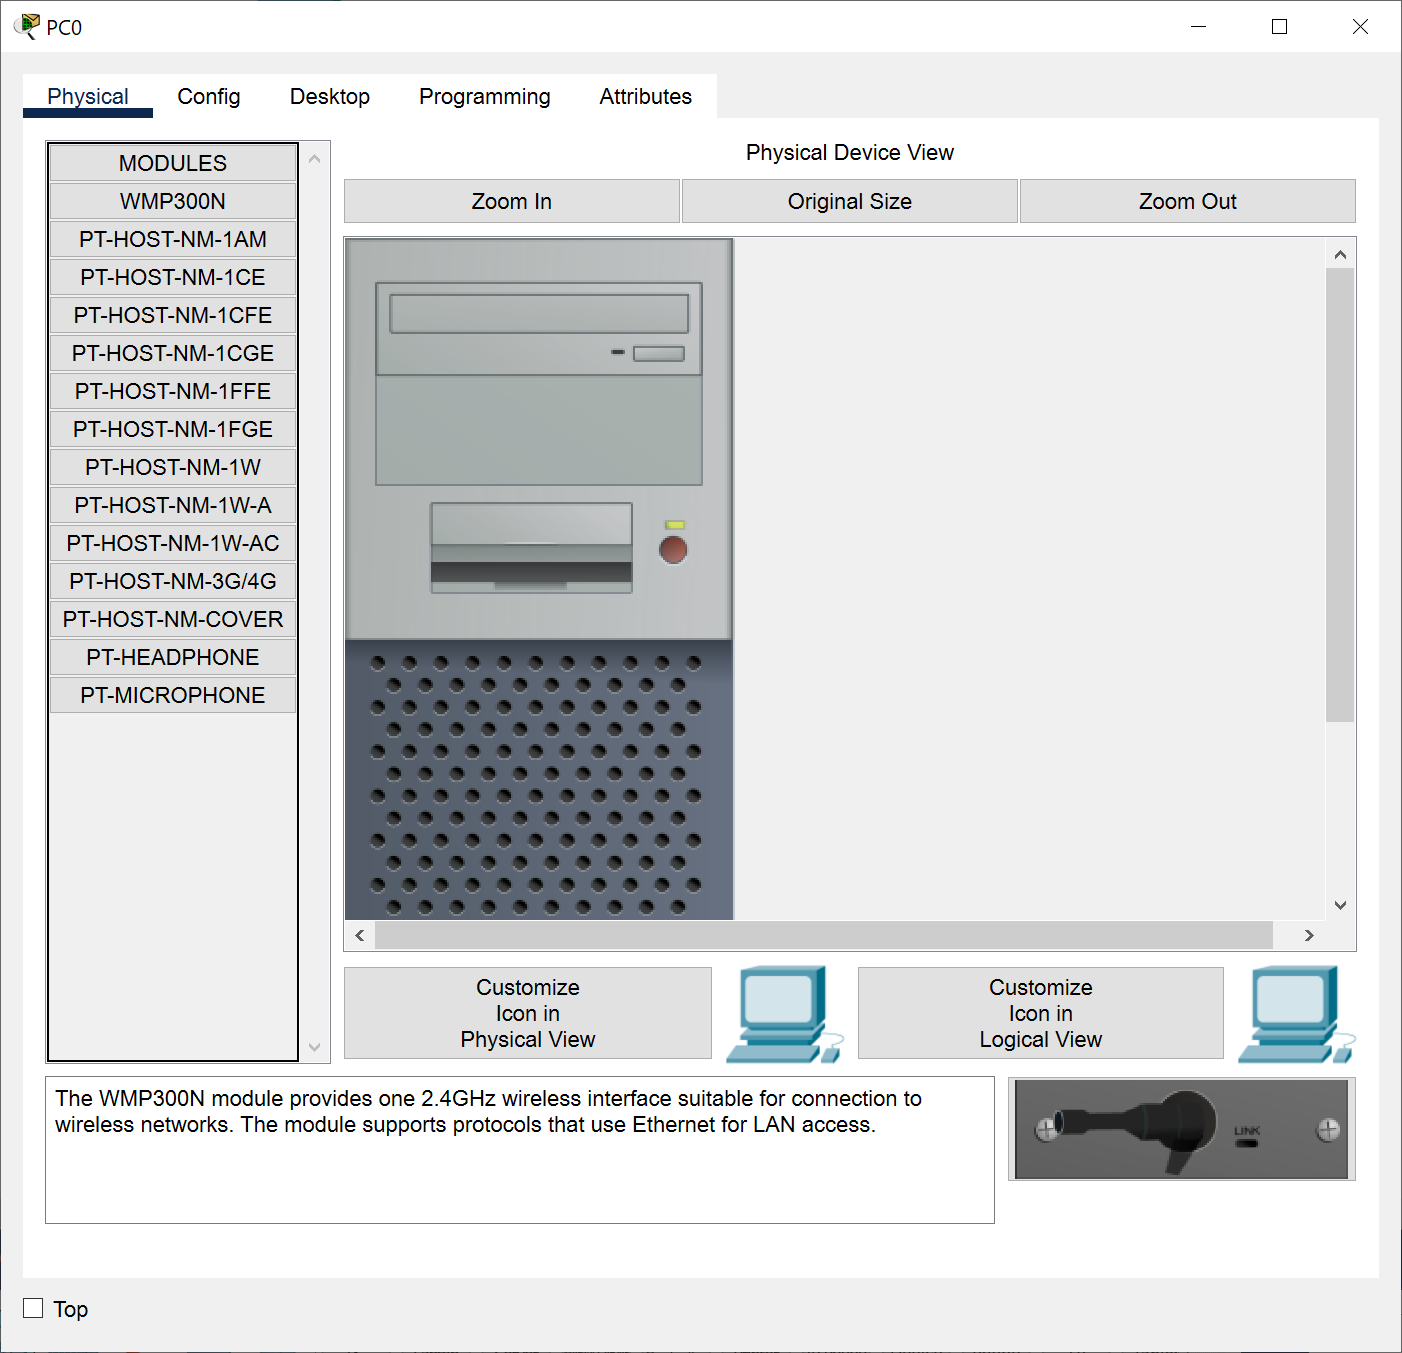
\includegraphics[width=13cm]{./step-by-step/3.PNG}
\clearpage

\noindent And we move ourselves in the \textvg{Config} tab \newline

\noindent 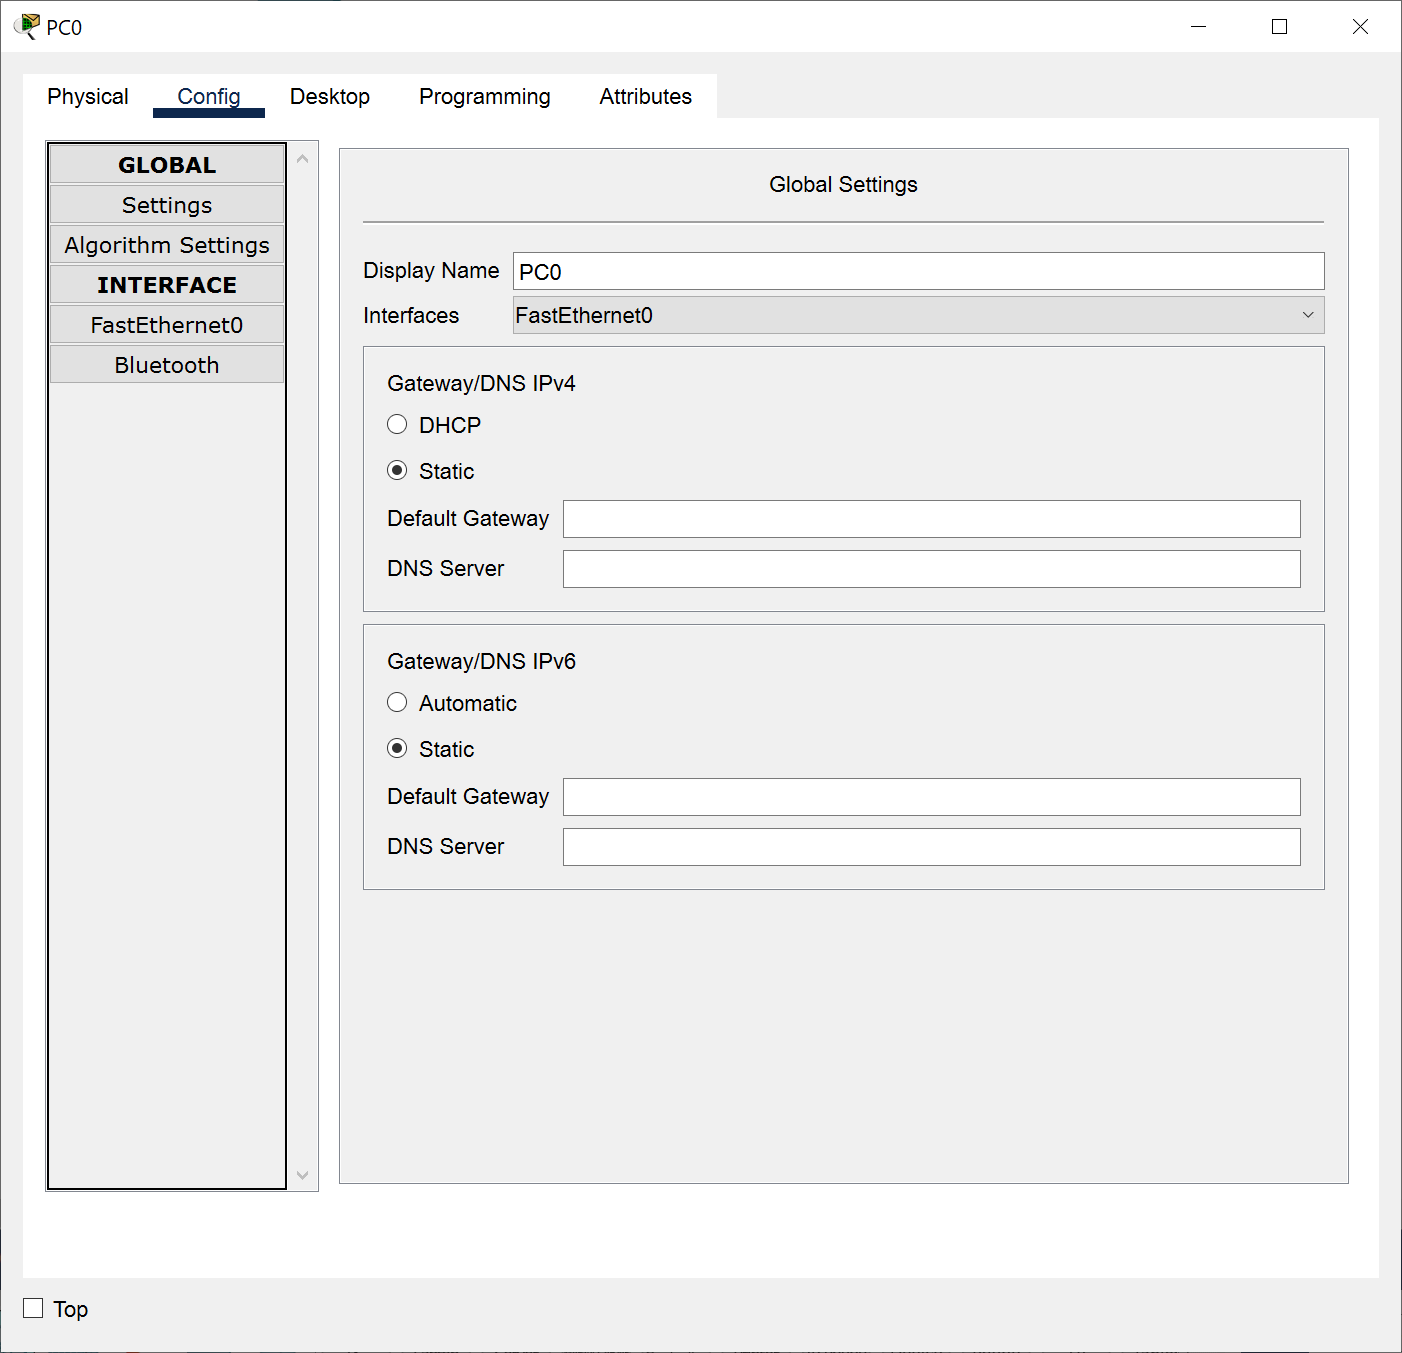
\includegraphics[width=13cm]{./step-by-step/4.PNG}
\clearpage

\noindent what we're gonna be looking later at is the IPV4 address \newline

\noindent 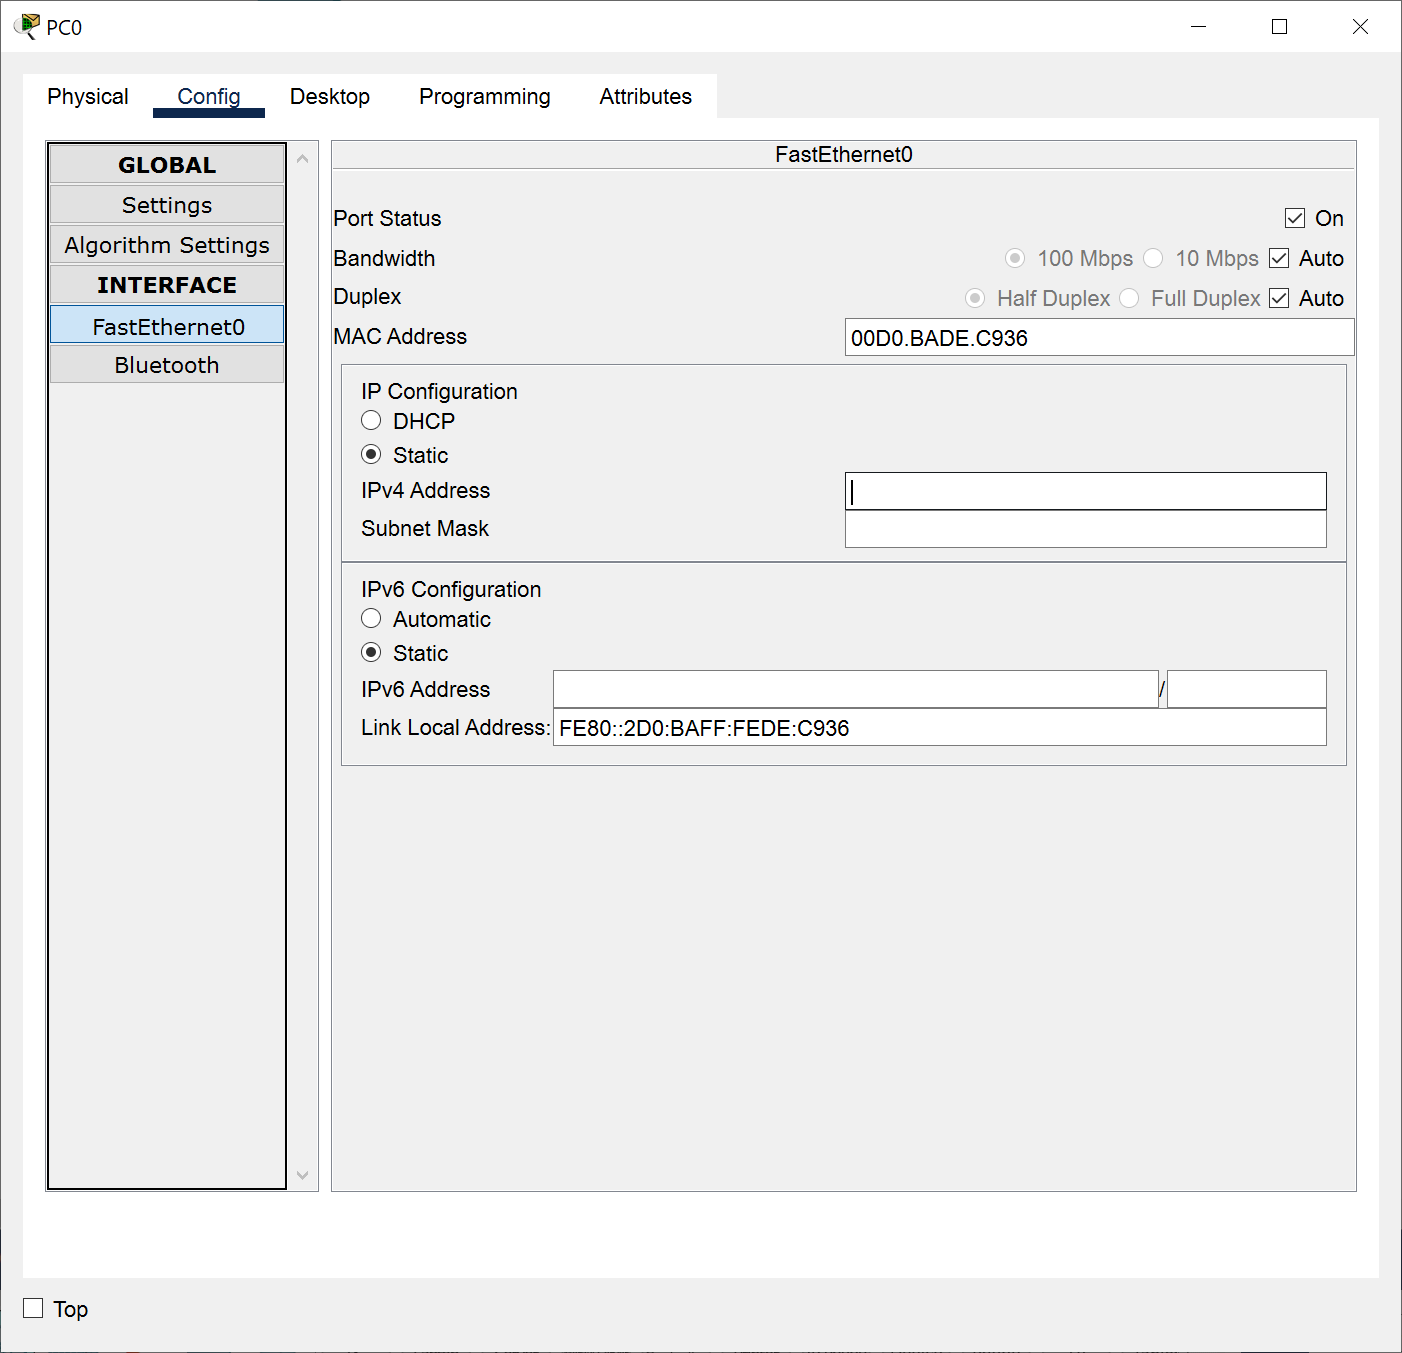
\includegraphics[width=13cm]{./step-by-step/5.PNG}
\clearpage

\noindent in the meantime let's  go in global and set the \textbf{IP Address} equal to this 

\[192.168.0.1\]

\noindent 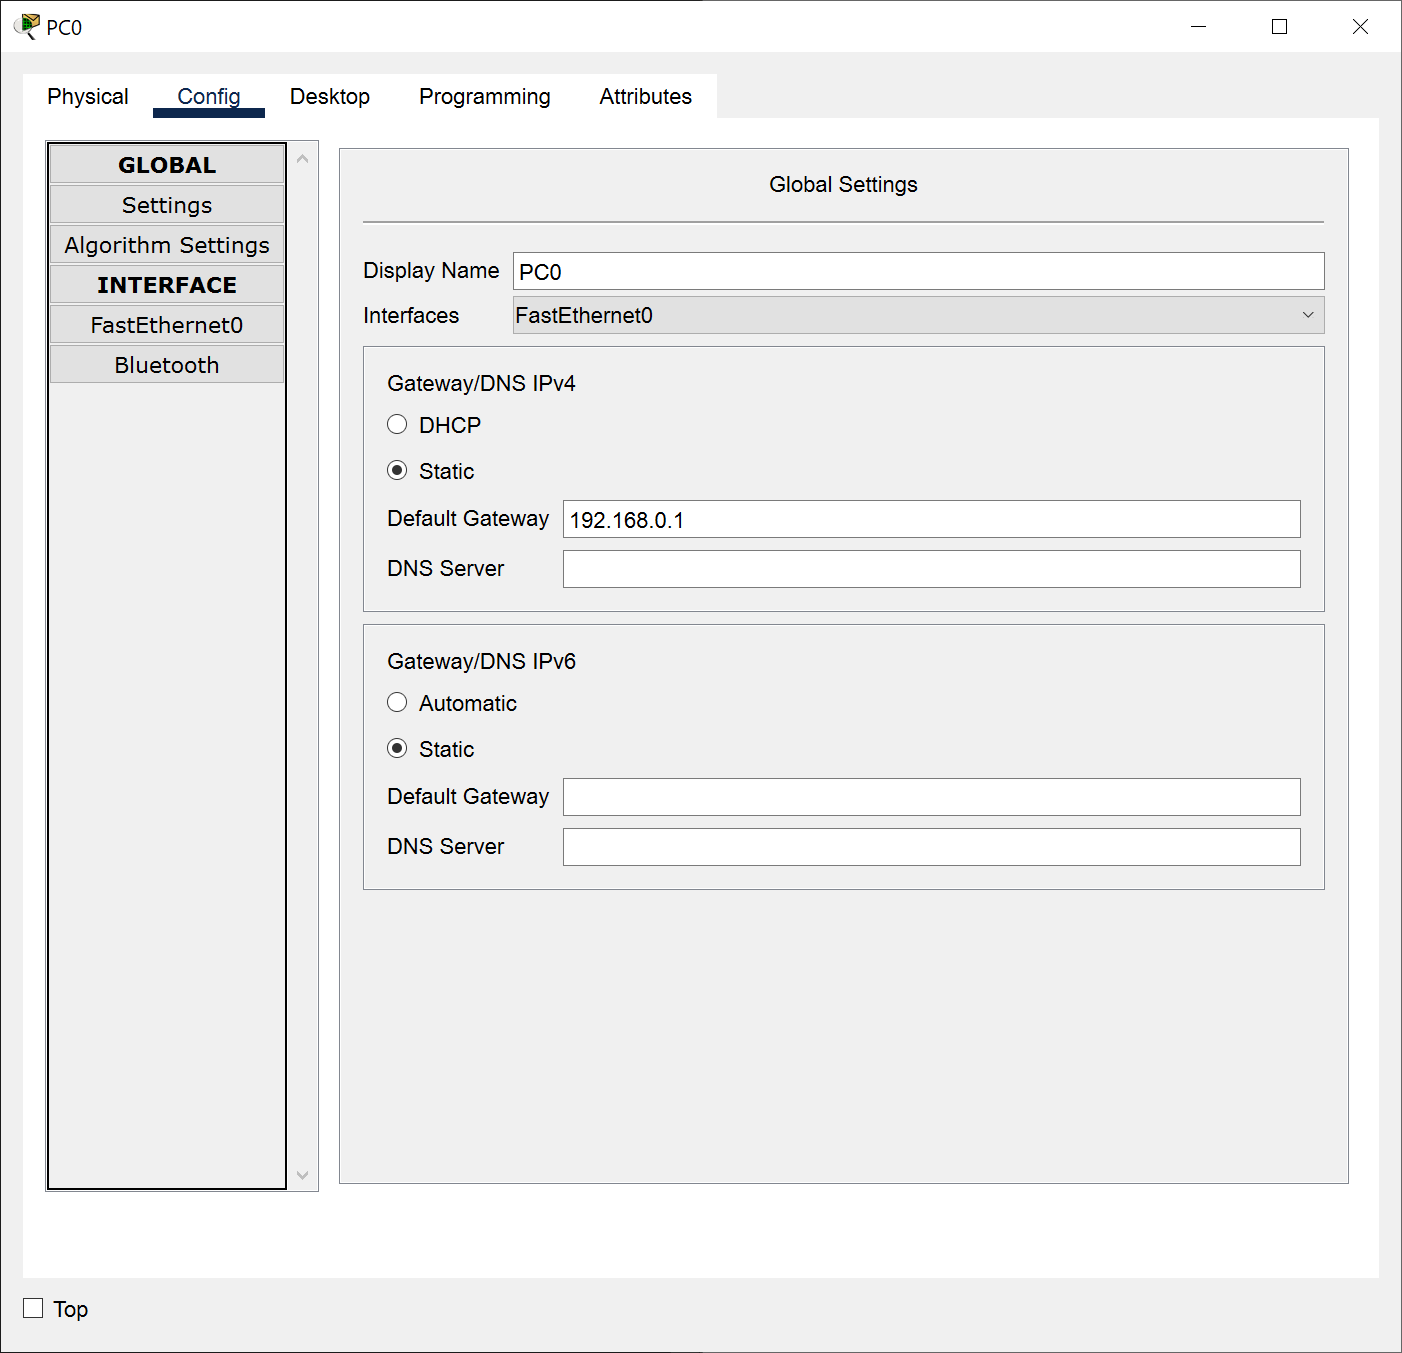
\includegraphics[width=13cm]{./step-by-step/6.PNG}
\clearpage

\noindent Now we add a new computer \newline

\noindent 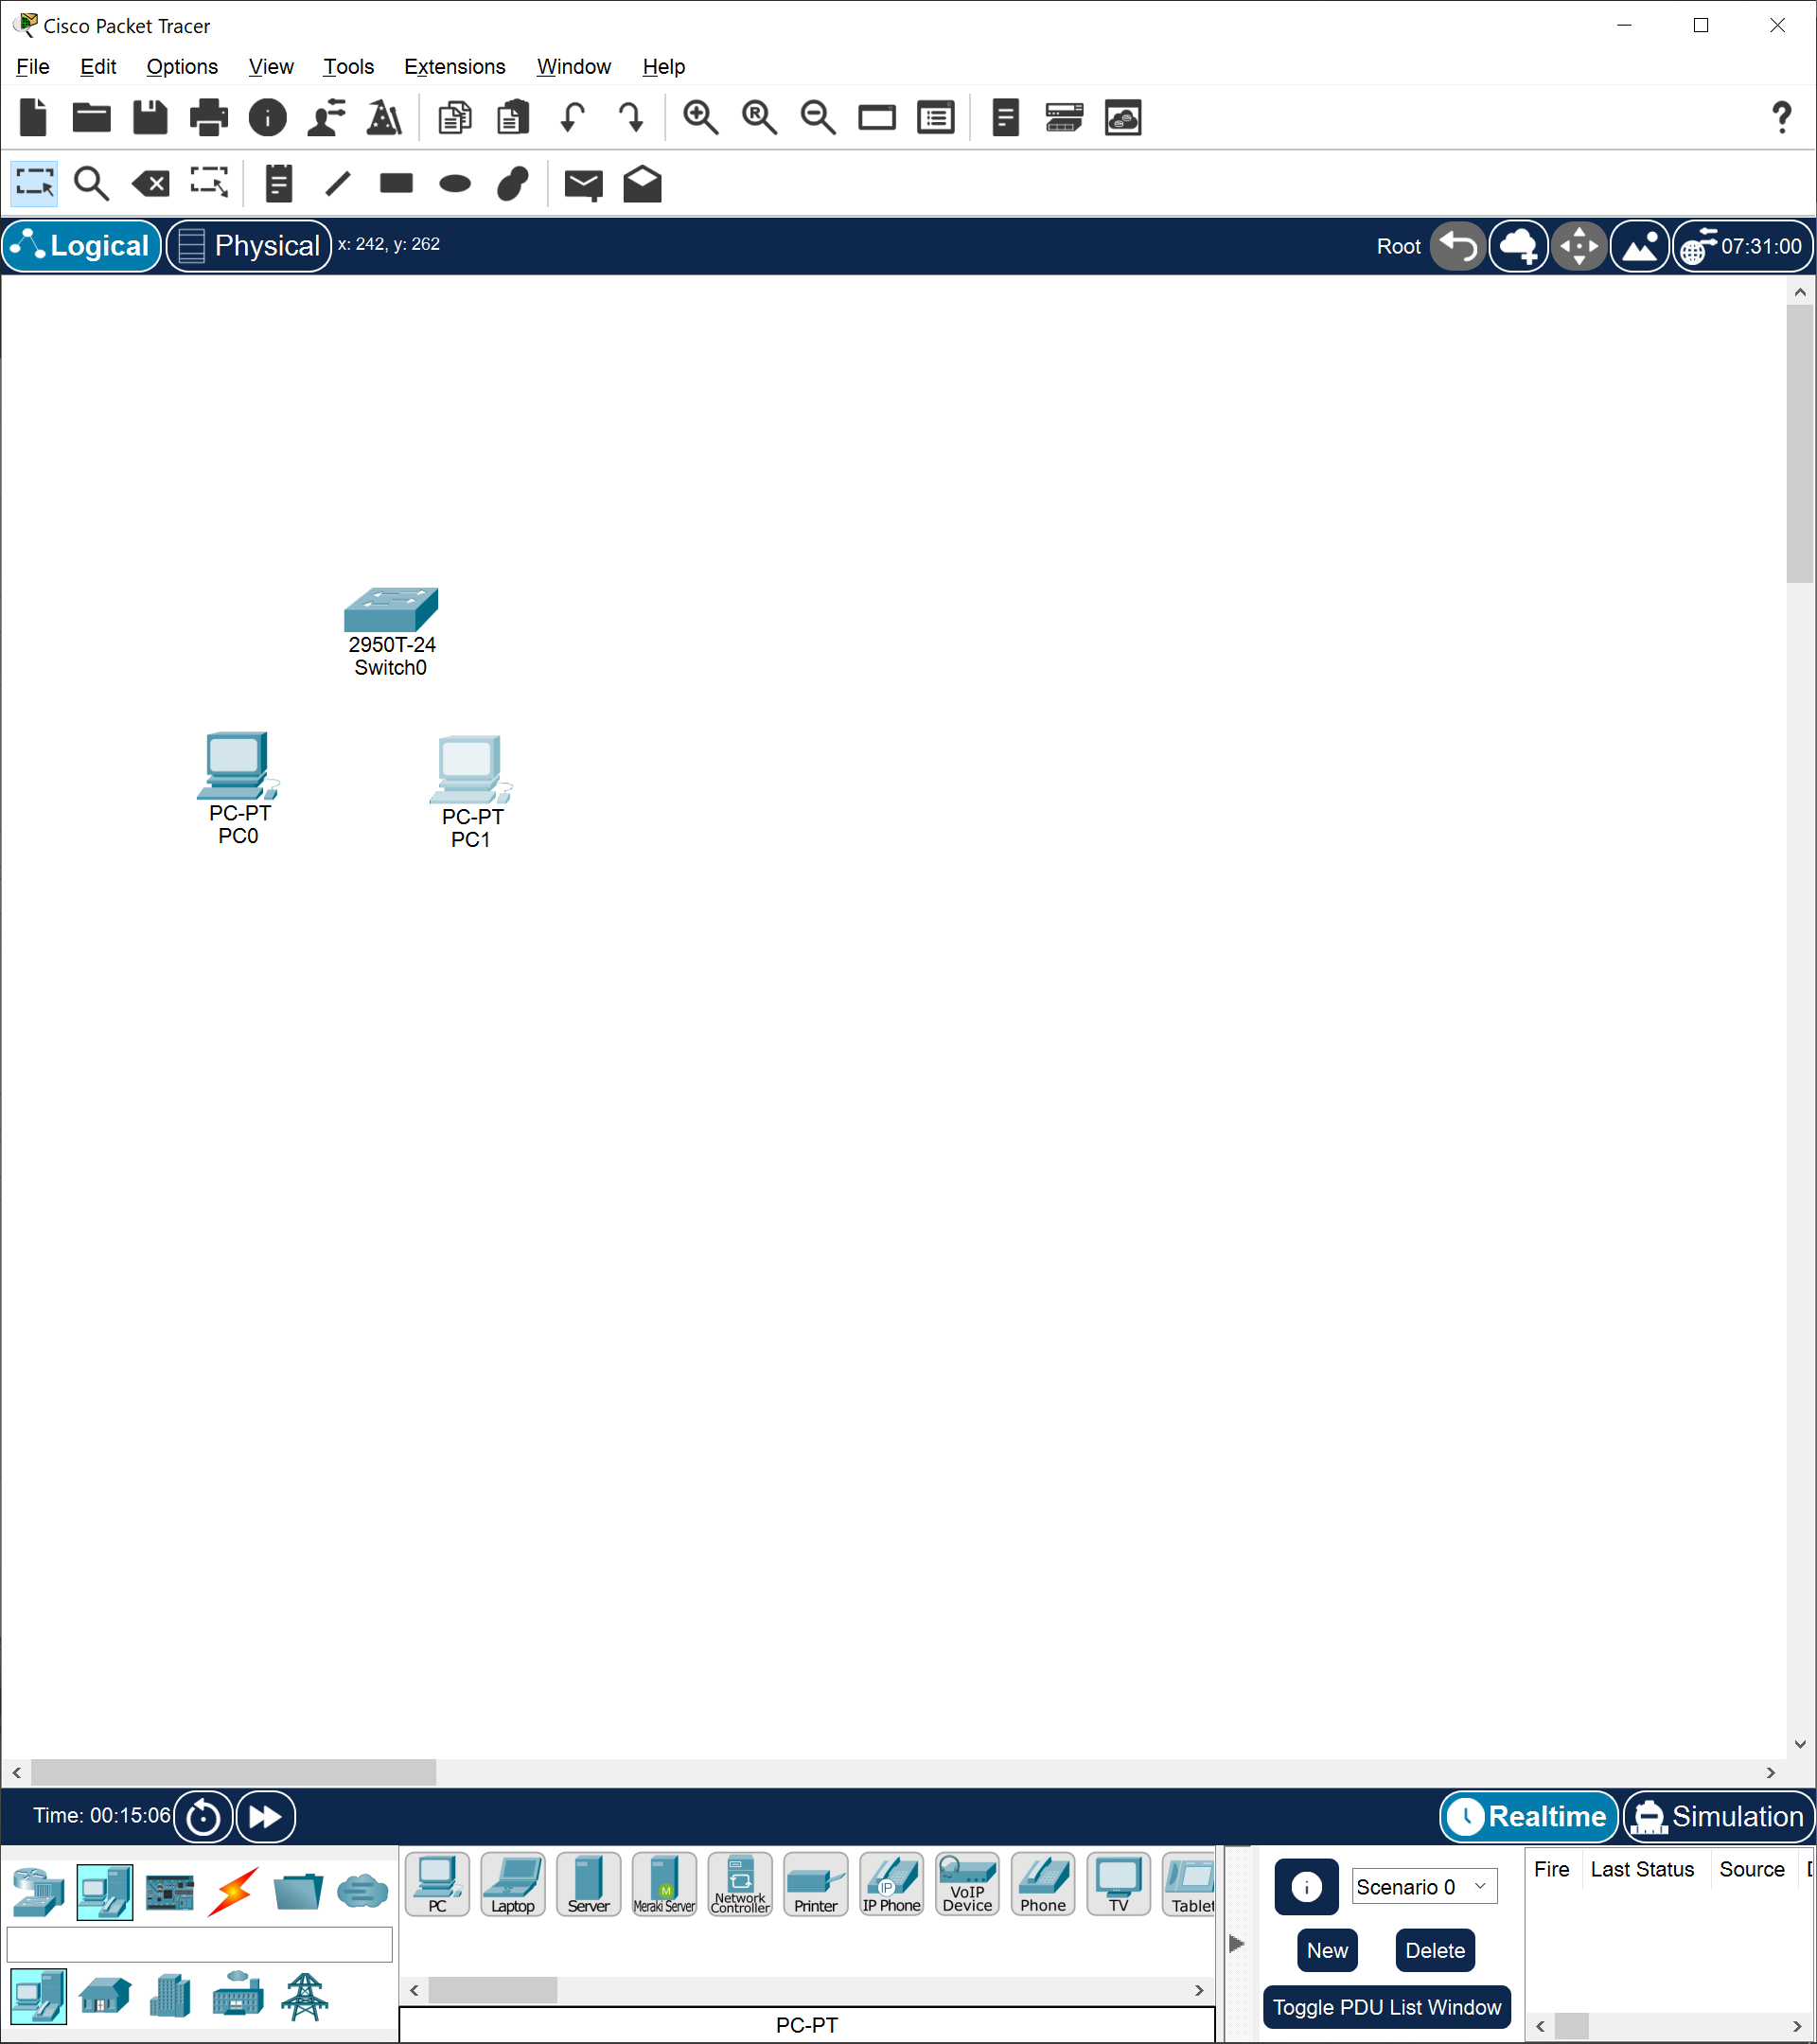
\includegraphics[width=13cm]{./step-by-step/7.PNG}
\clearpage


\noindent We link the switch to the first computer and wait for all lights to go green \newline

\noindent 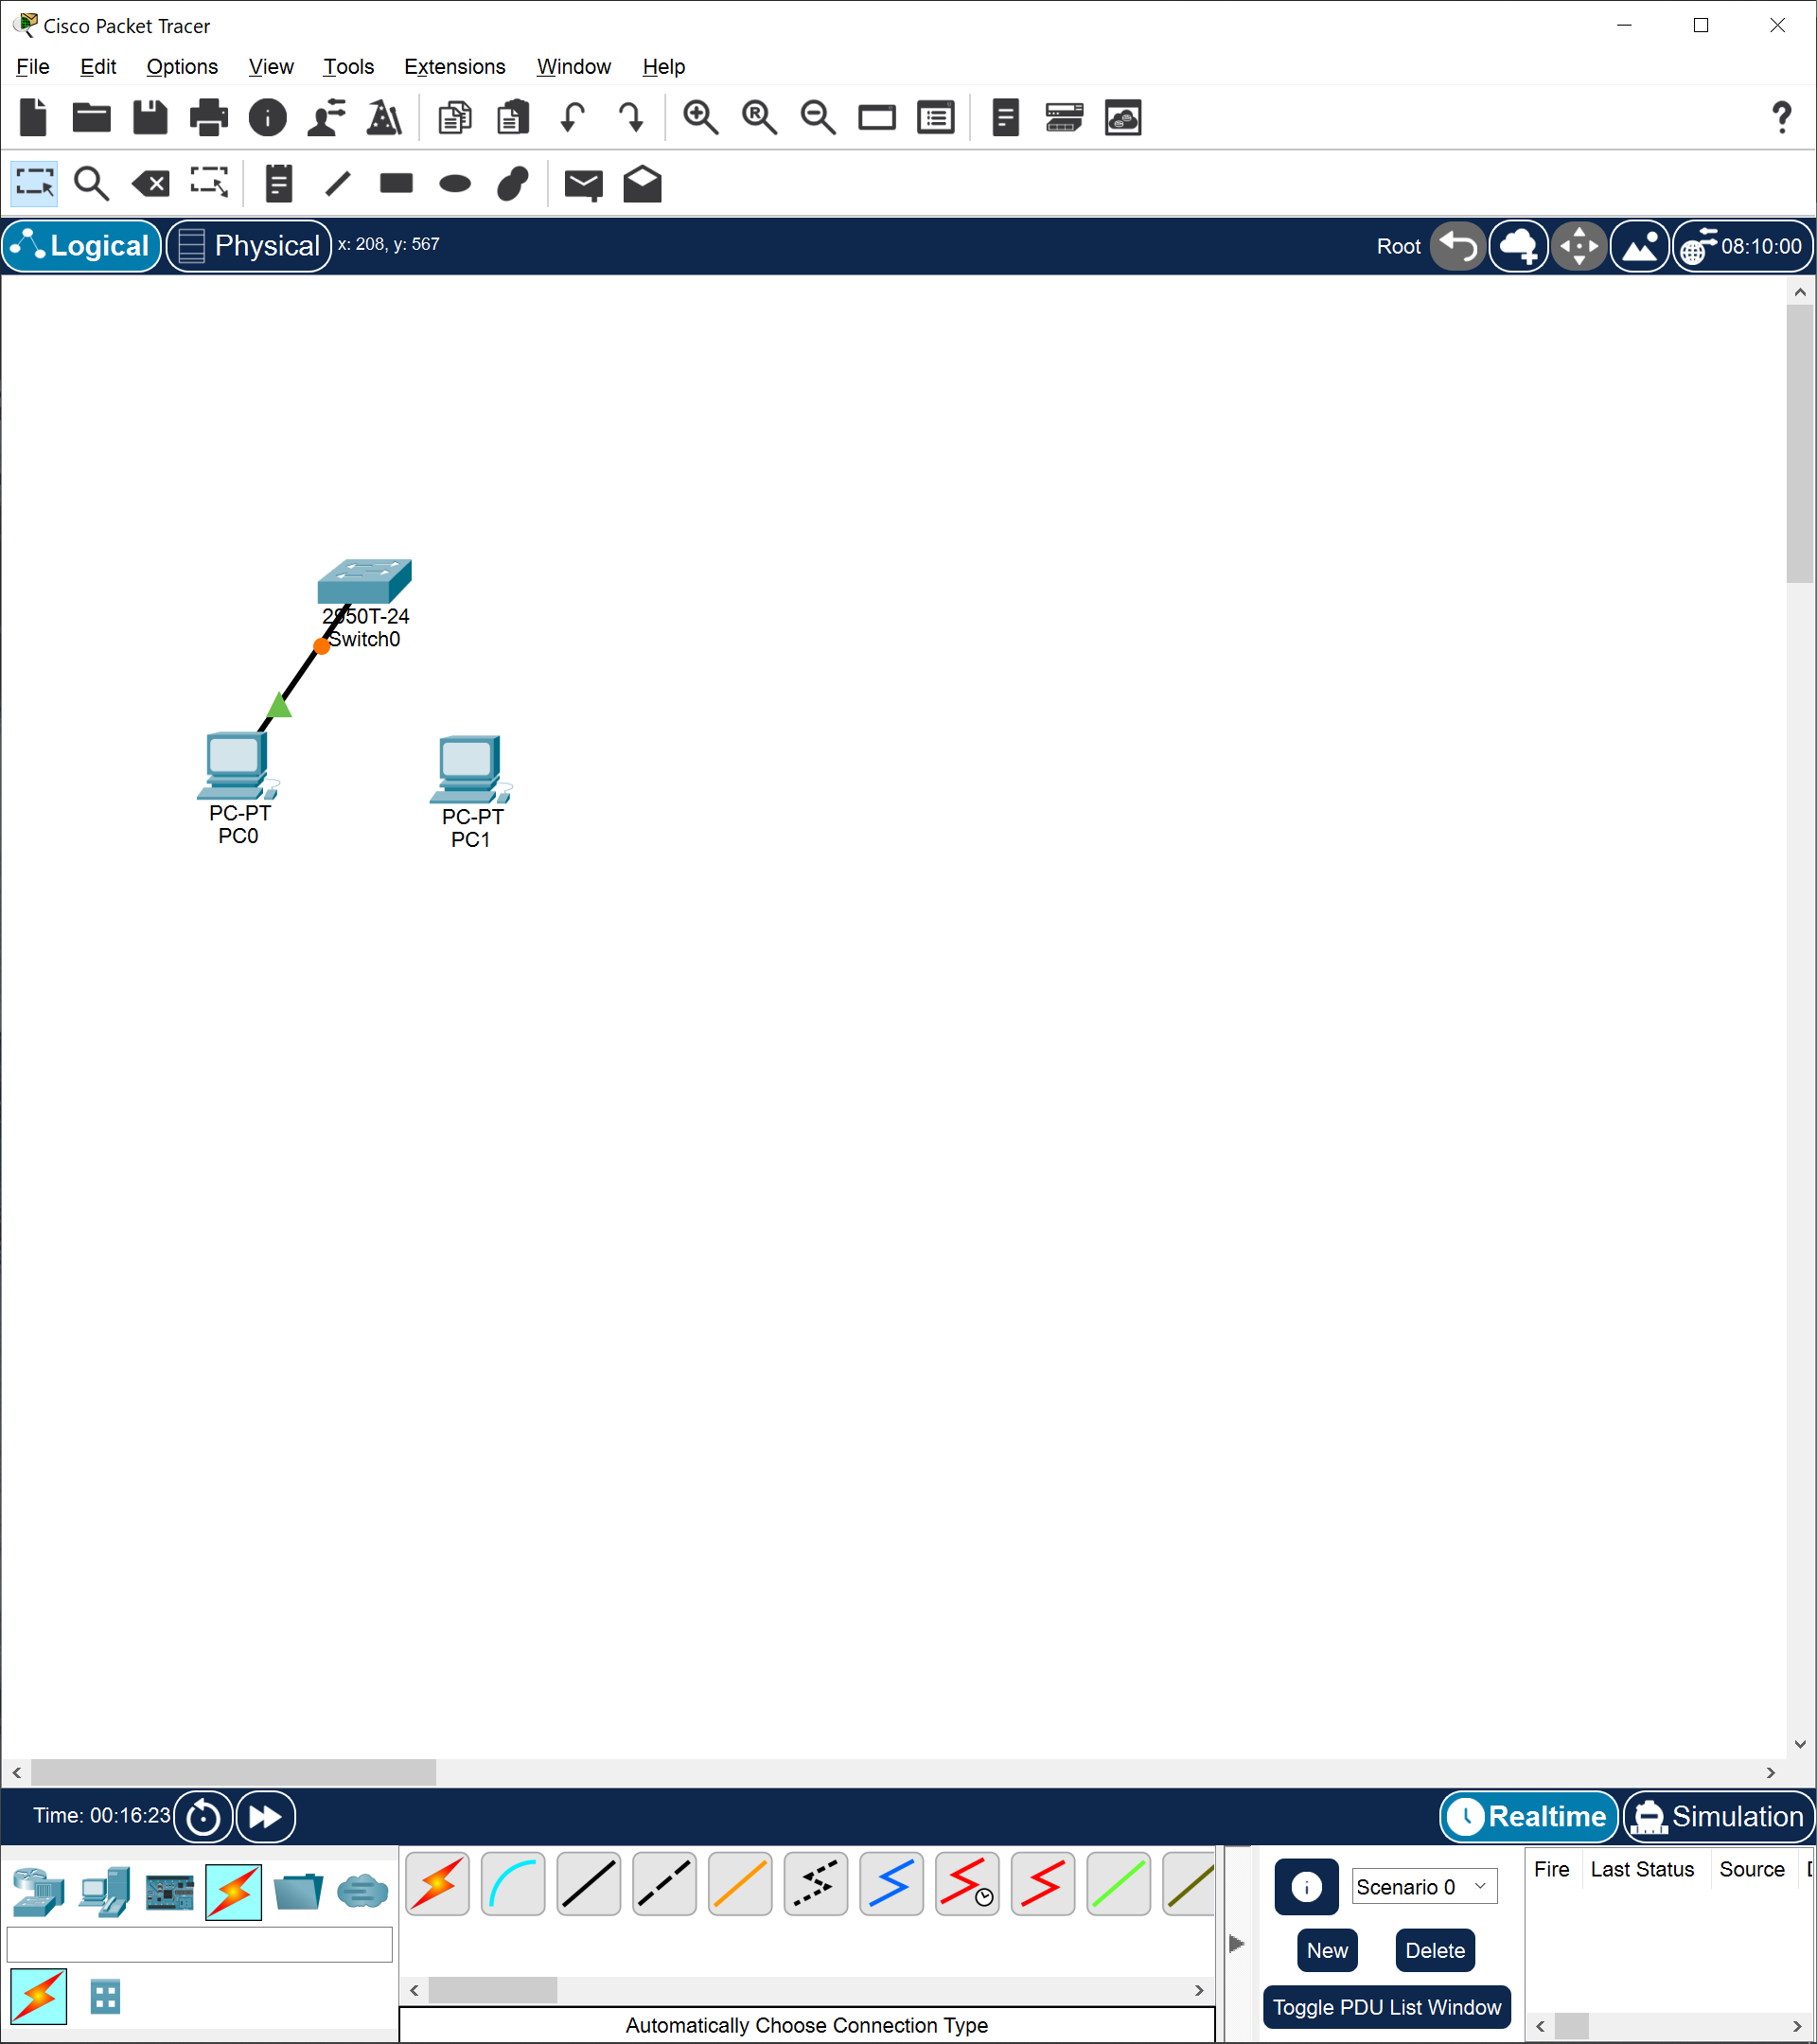
\includegraphics[width=13cm]{./step-by-step/8.PNG}
\clearpage

\noindent Link the switch to the second computer and wait for this link to go all green as well \newline

\noindent 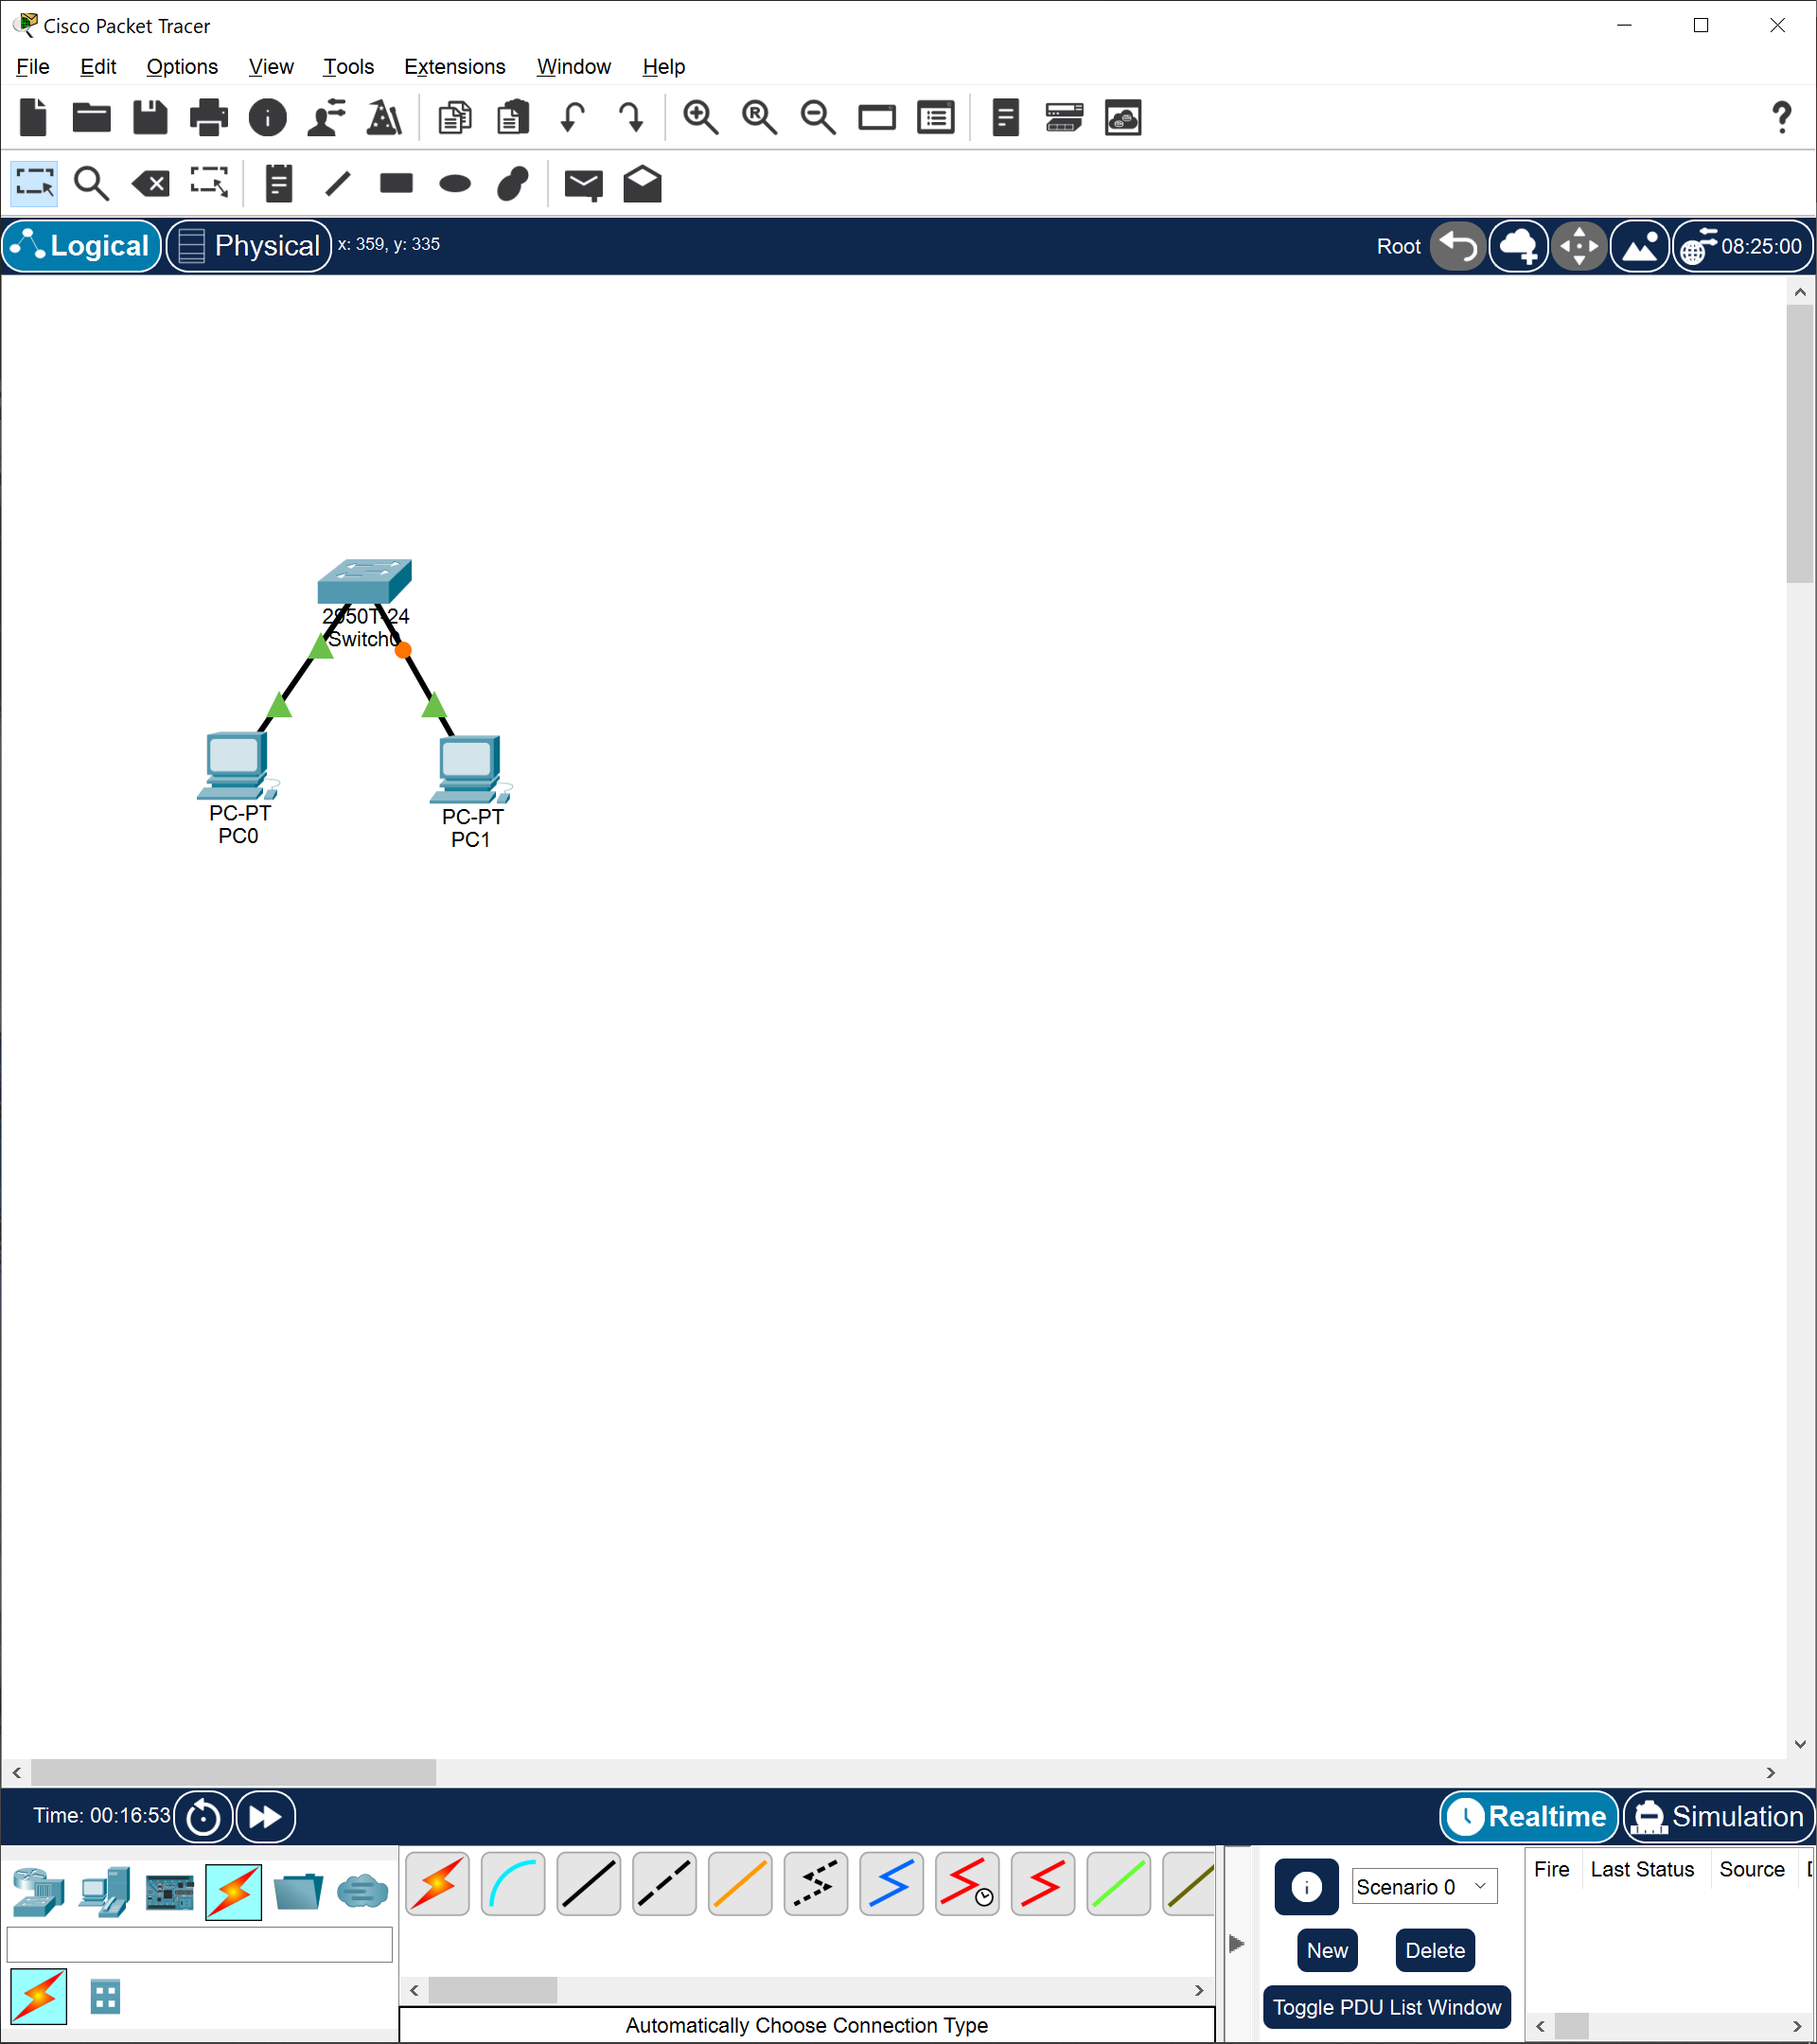
\includegraphics[width=13cm]{./step-by-step/9.PNG}
\clearpage

\noindent Now it's all green which makes us happy \newline

\noindent 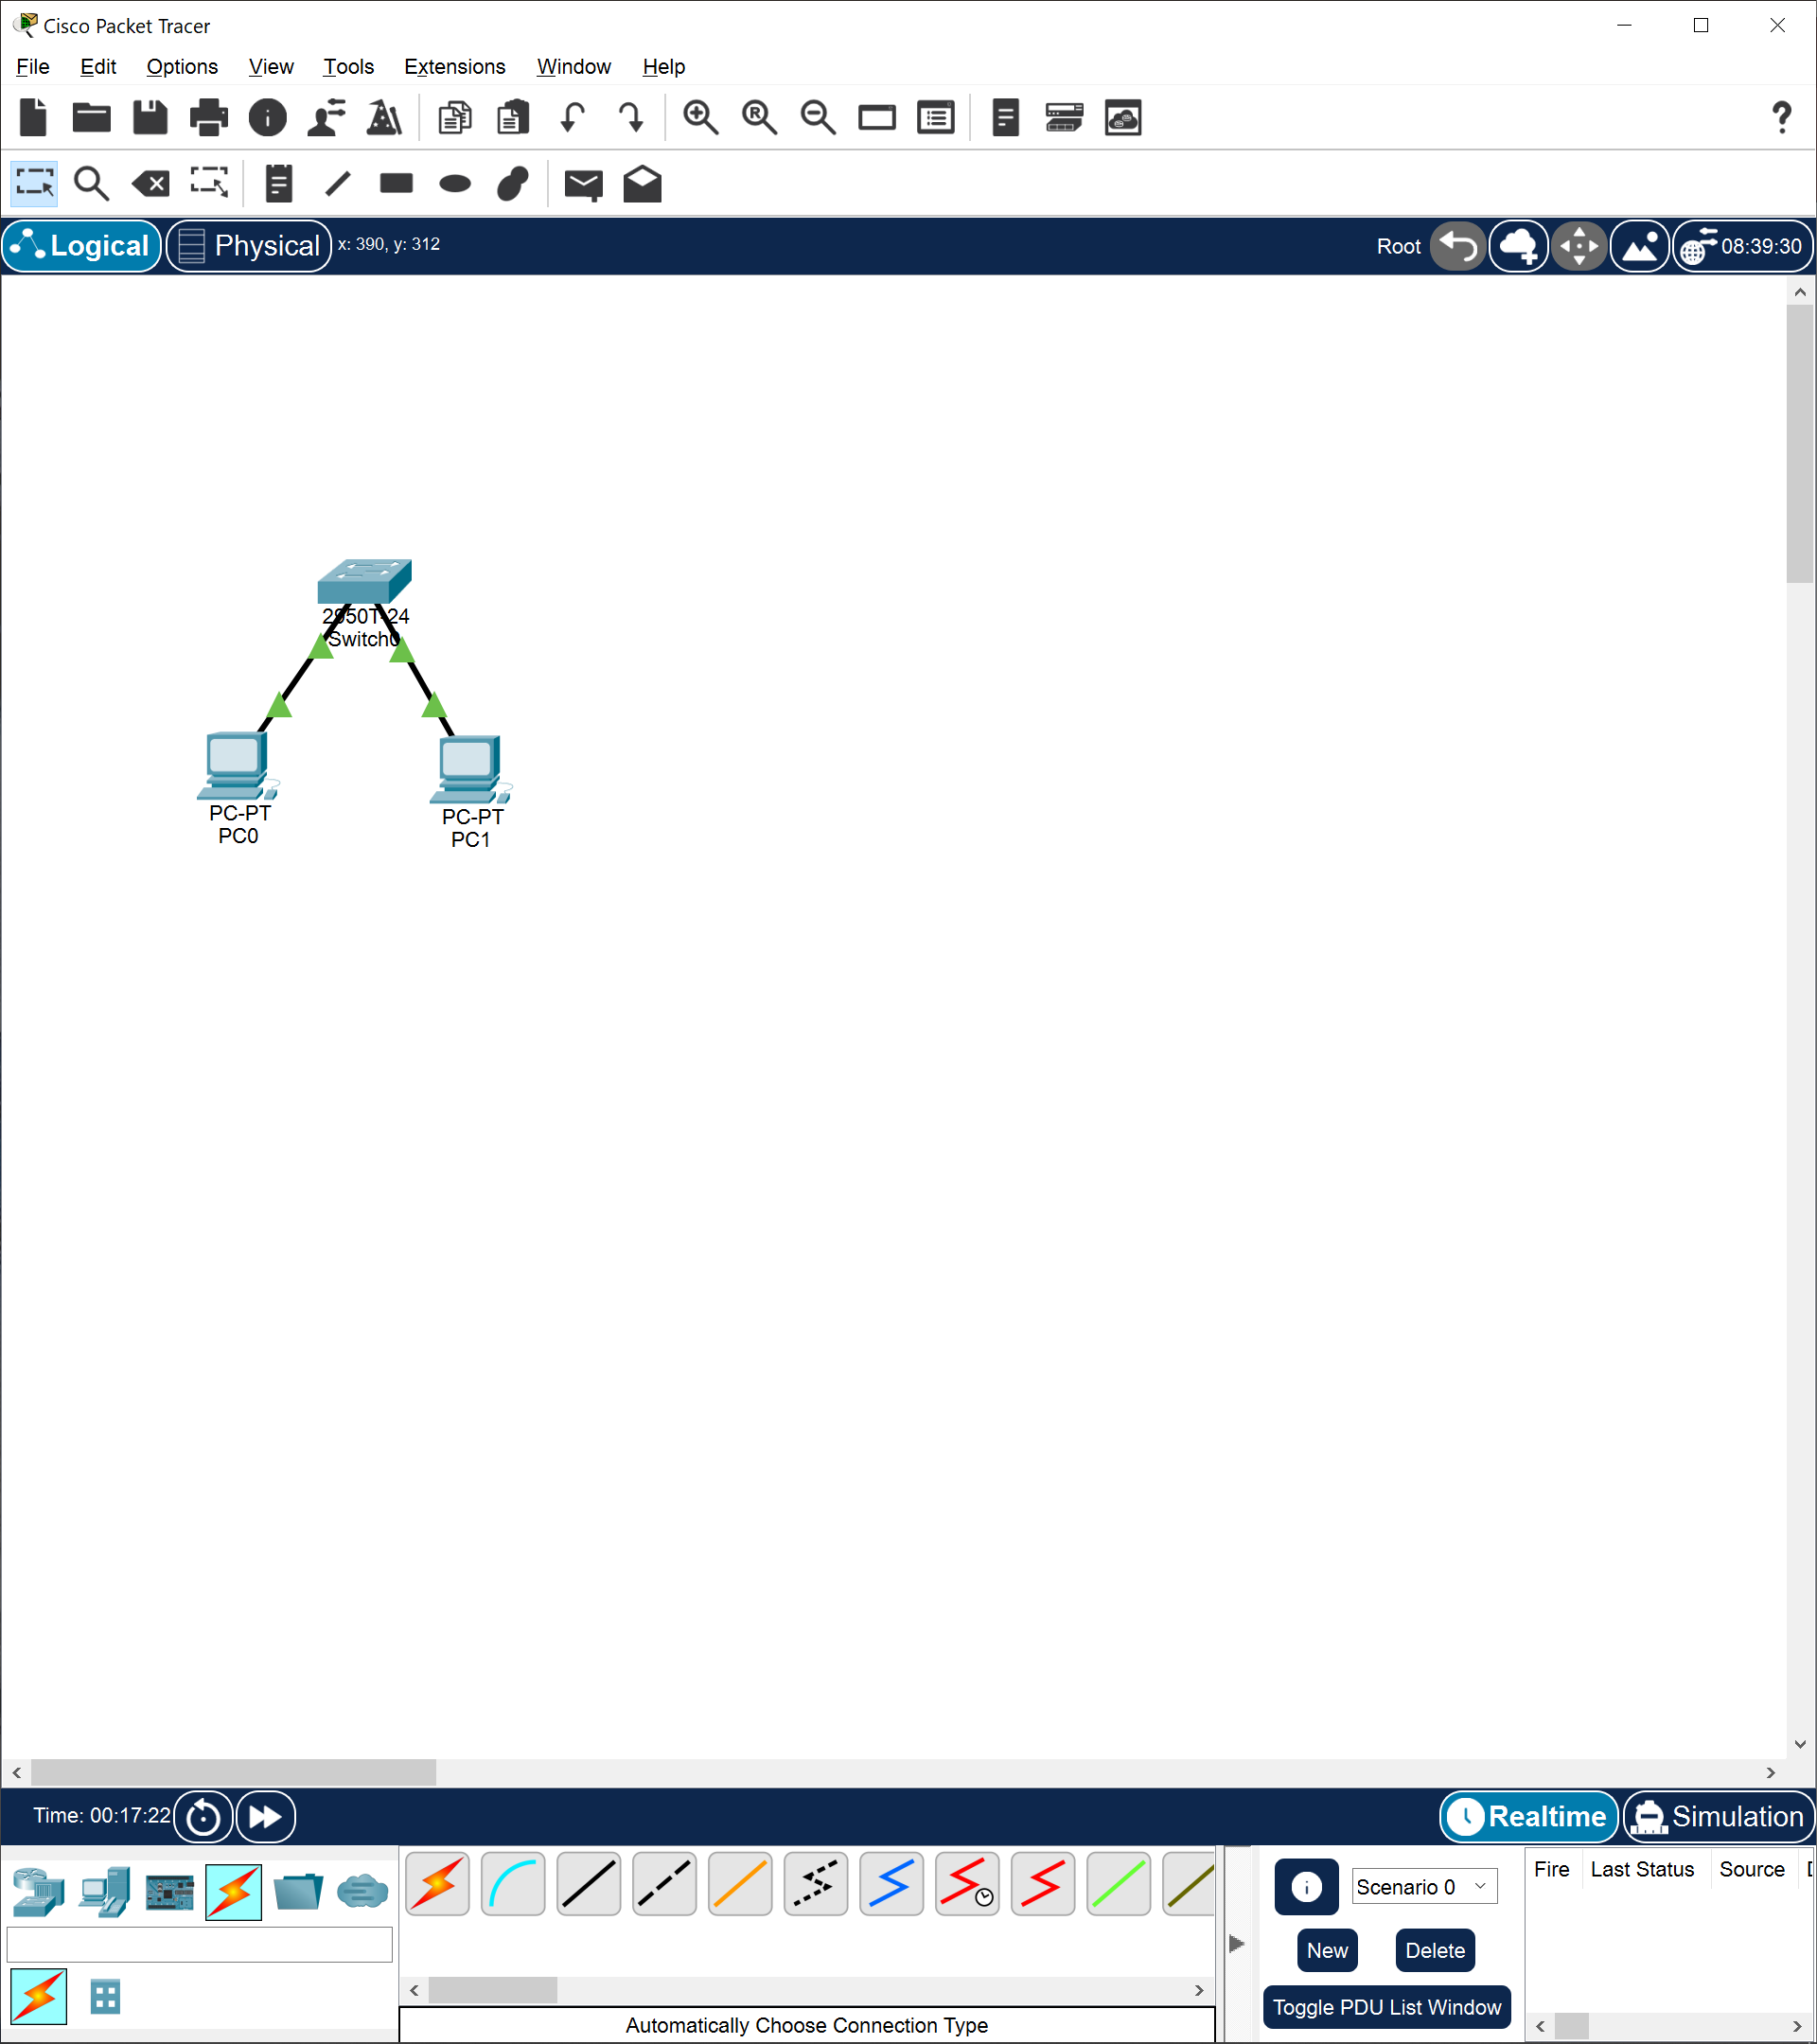
\includegraphics[width=13cm]{./step-by-step/10.PNG}
\clearpage

\noindent Let's add a router \newline

\noindent 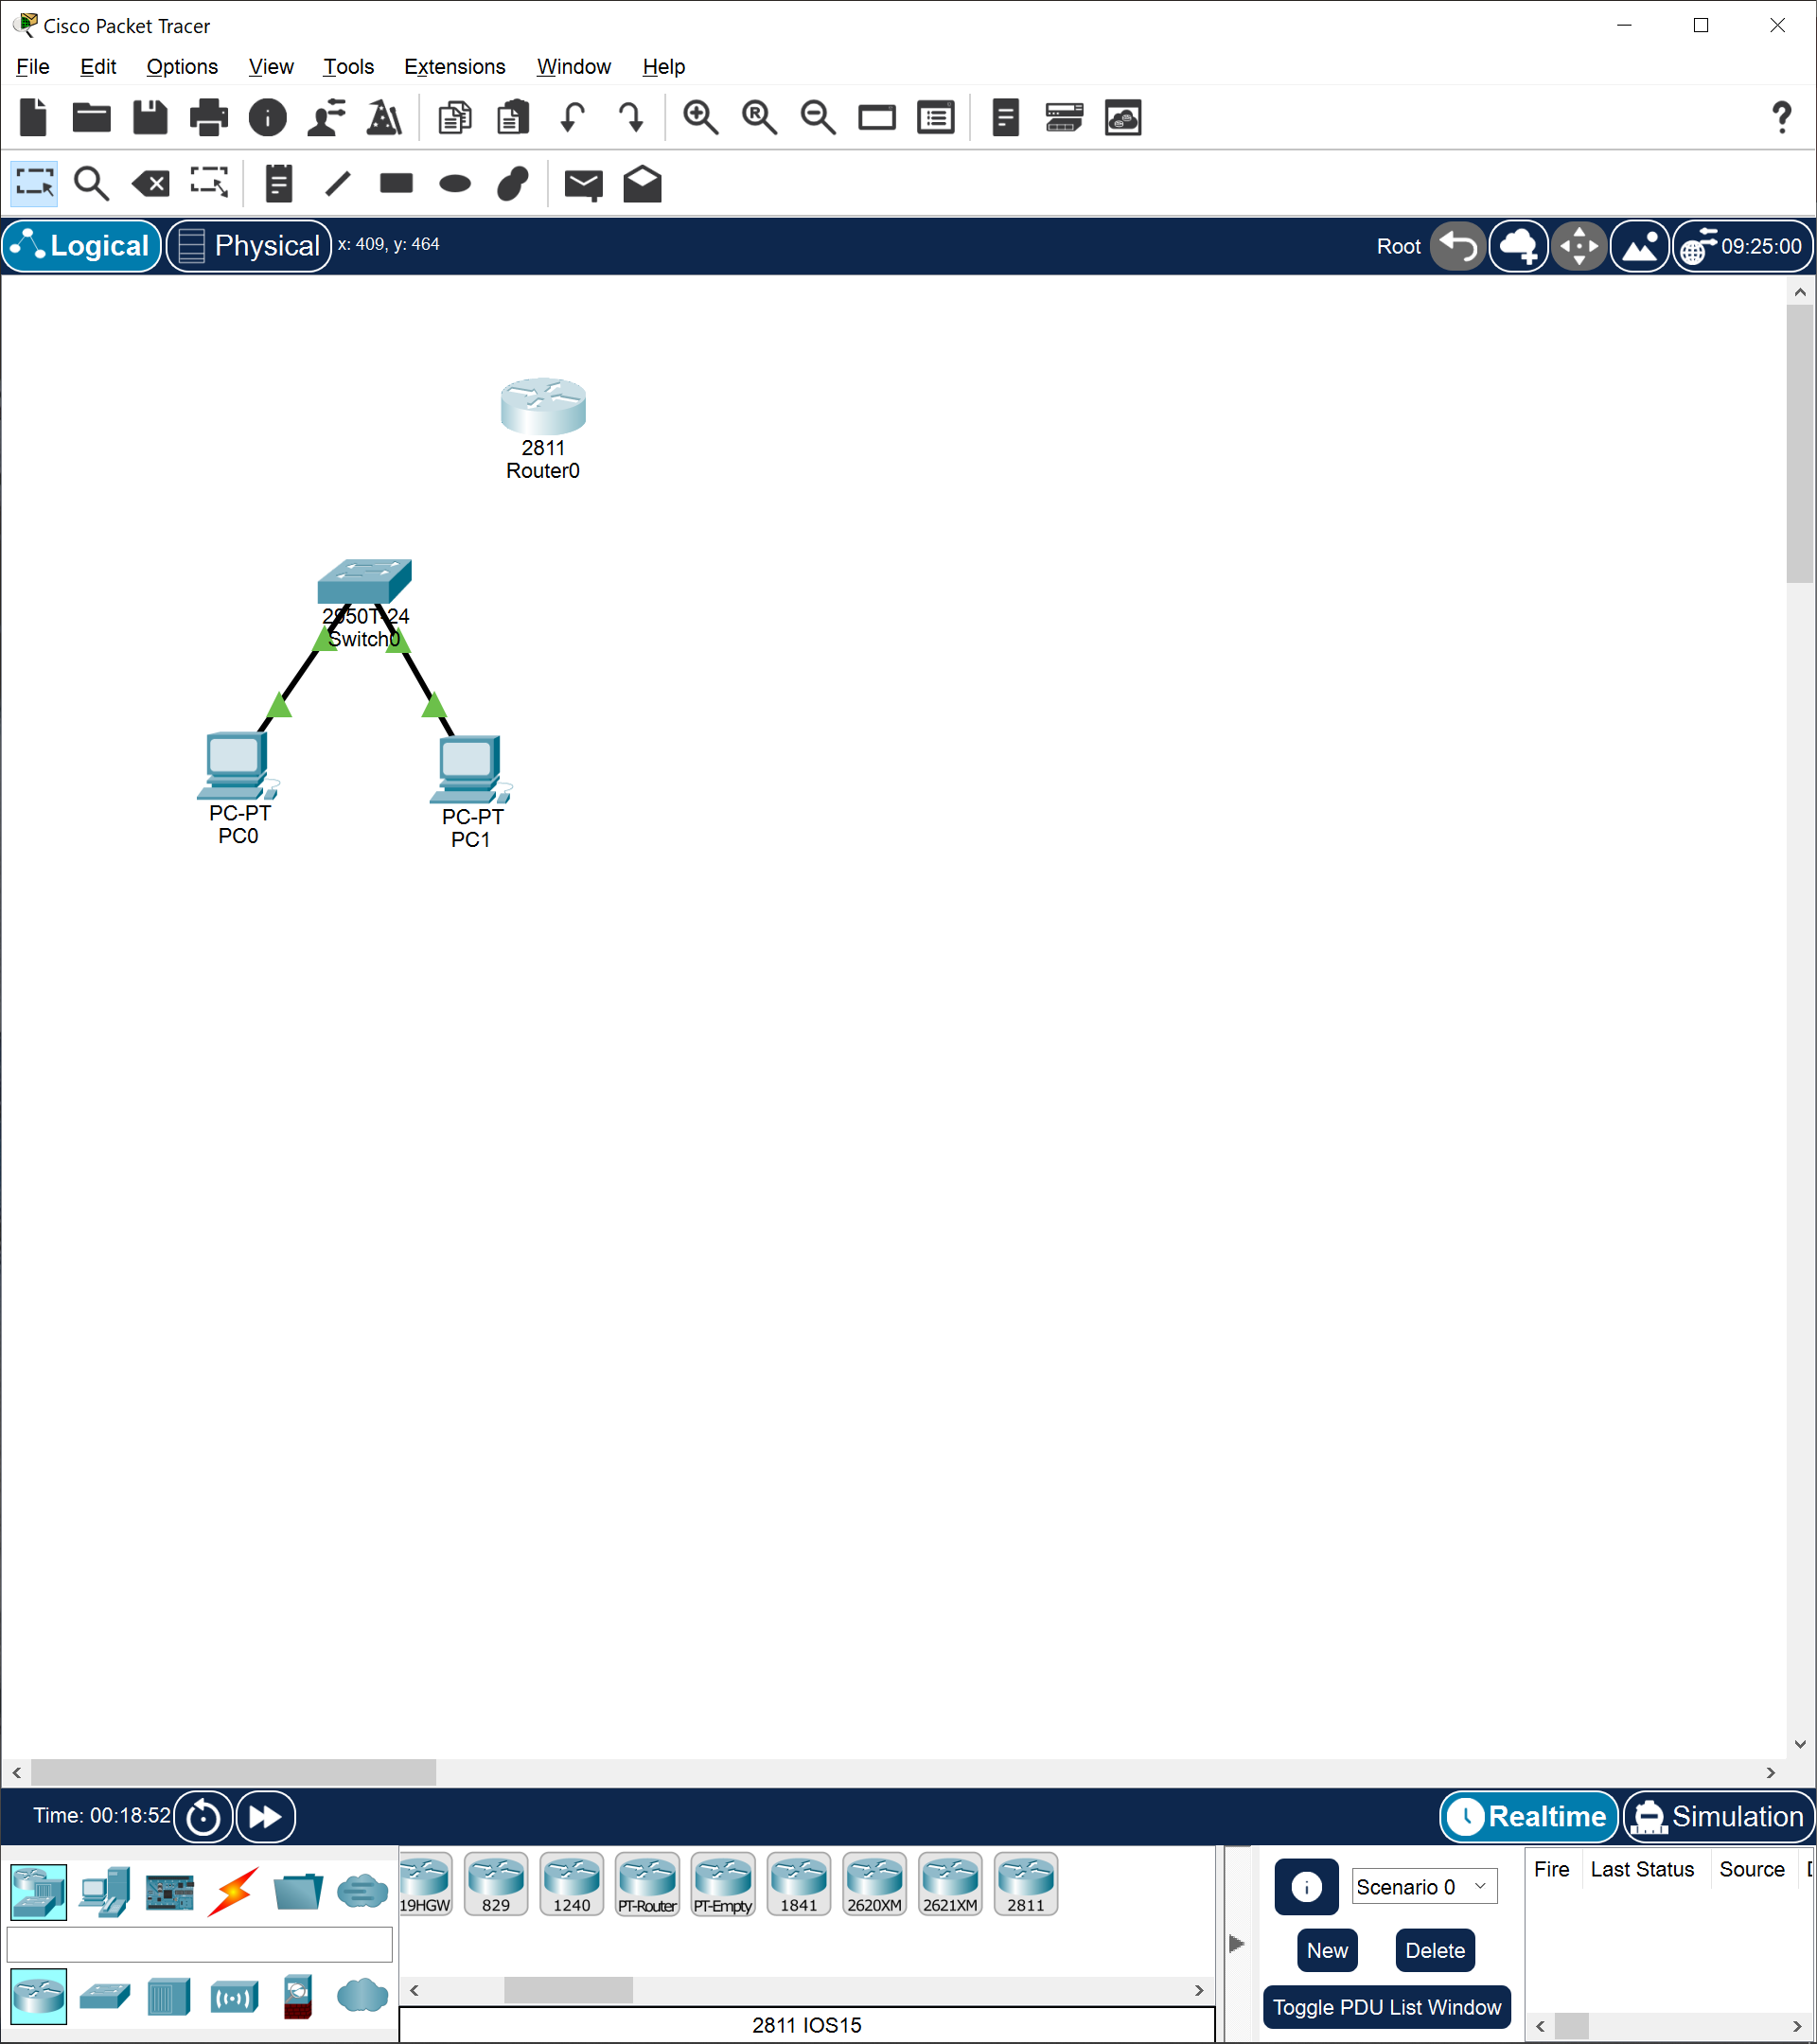
\includegraphics[width=13cm]{./step-by-step/11.PNG}
\clearpage

\noindent Let's link the router to the first computer \newline

\noindent 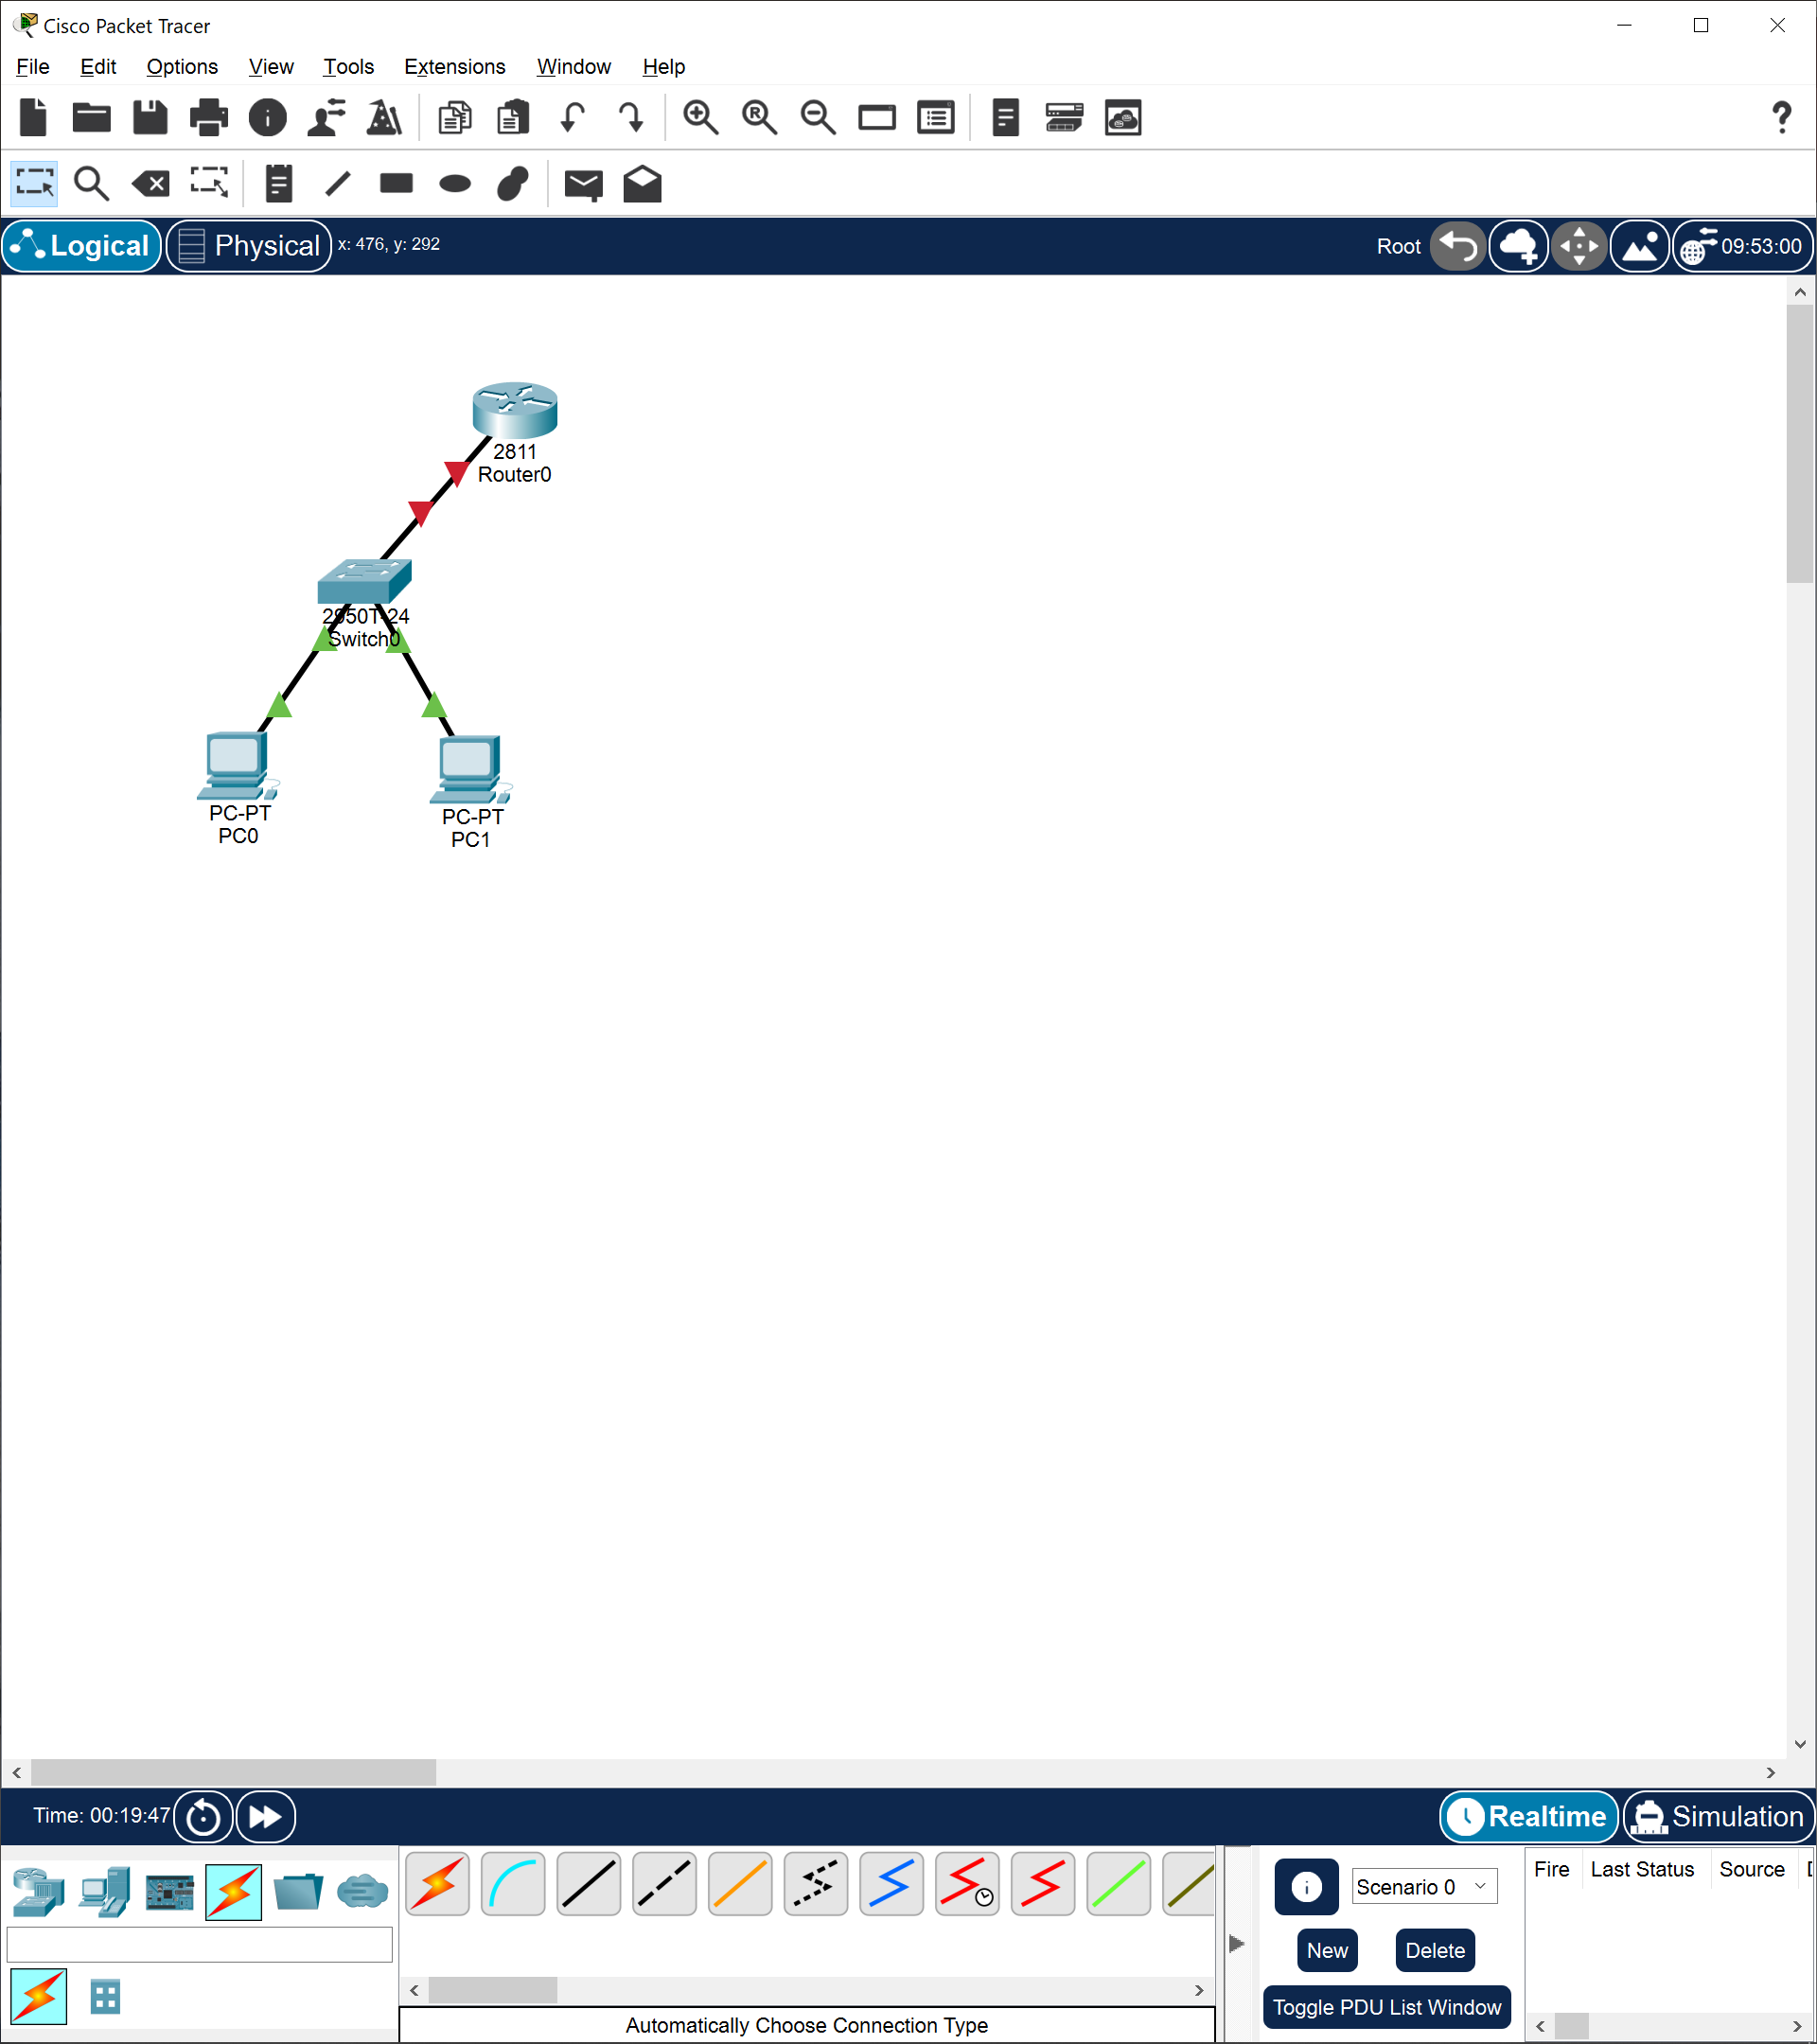
\includegraphics[width=13cm]{./step-by-step/12.PNG}
\clearpage

\noindent If you click on the router, in the config tab there is a box you need to check. That box will emulate the router being powered on \newline

\noindent 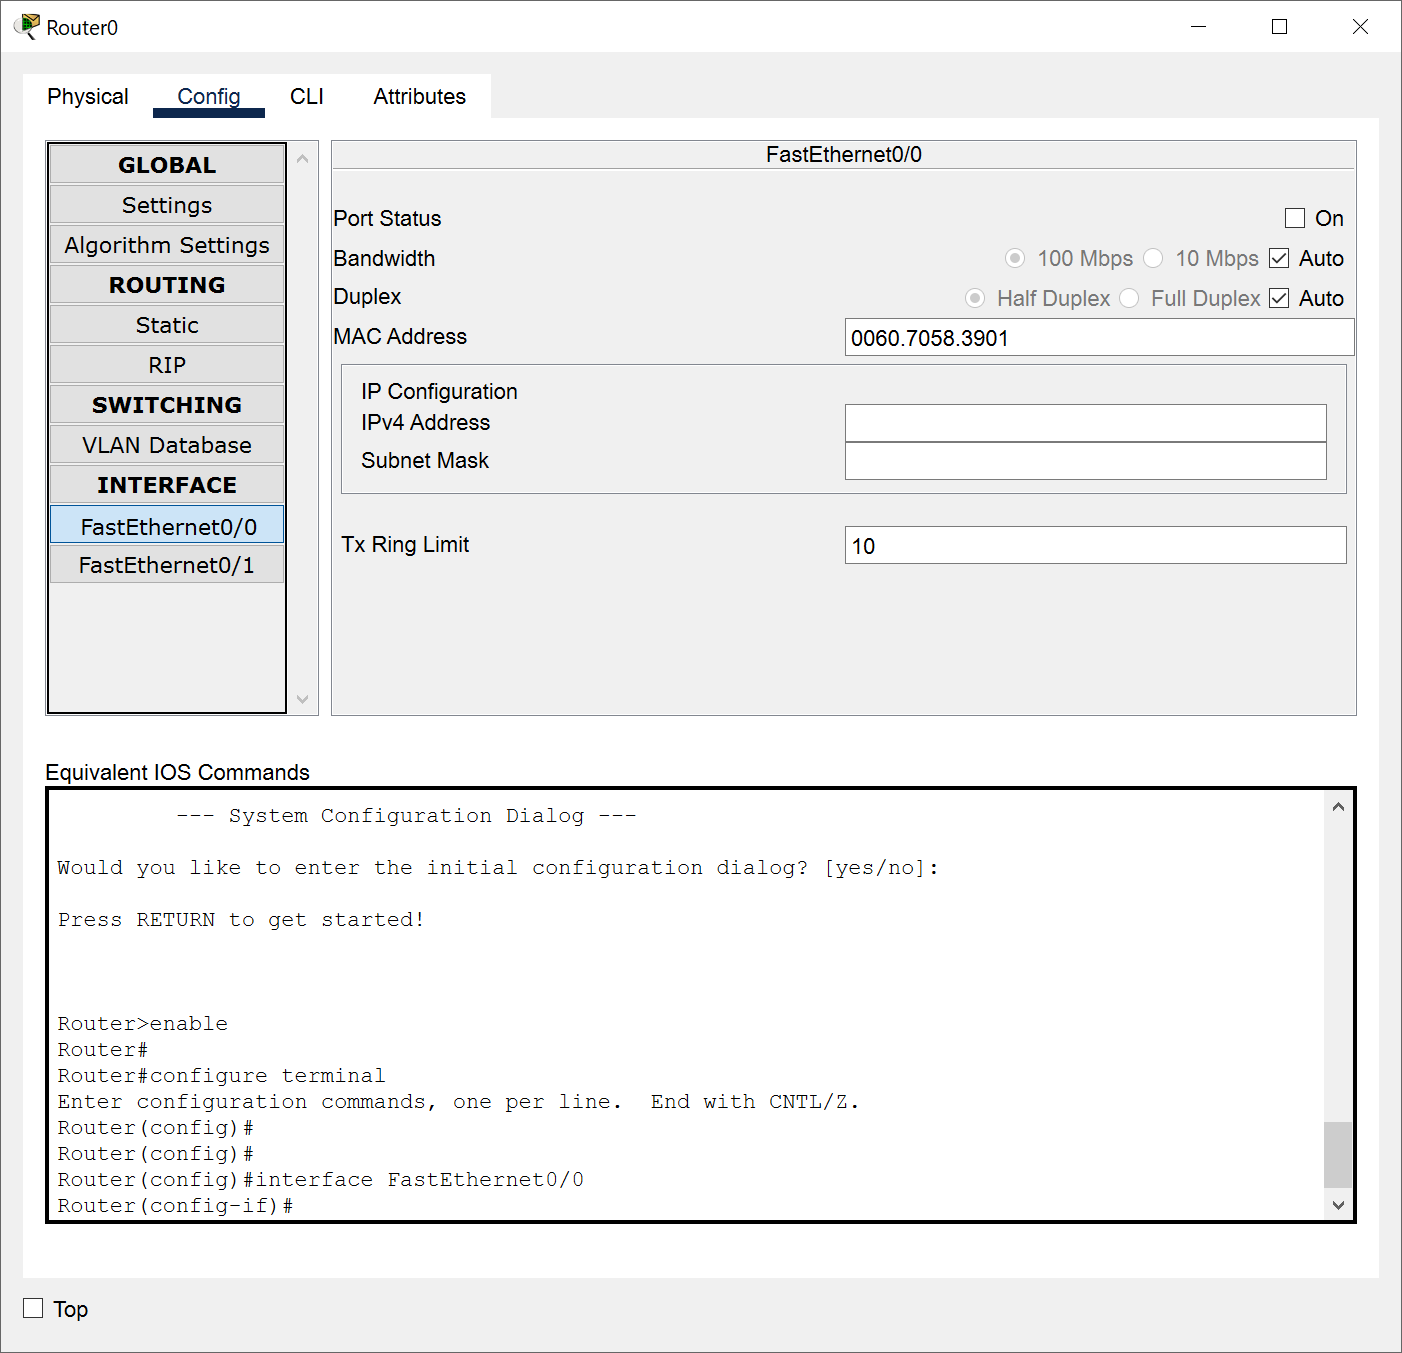
\includegraphics[width=13cm]{./step-by-step/13.PNG}
\clearpage


\noindent Once you click in the box a small tick will appear in it. This means the box is ticked and the function that box is proving is now being turned on \newline

\noindent 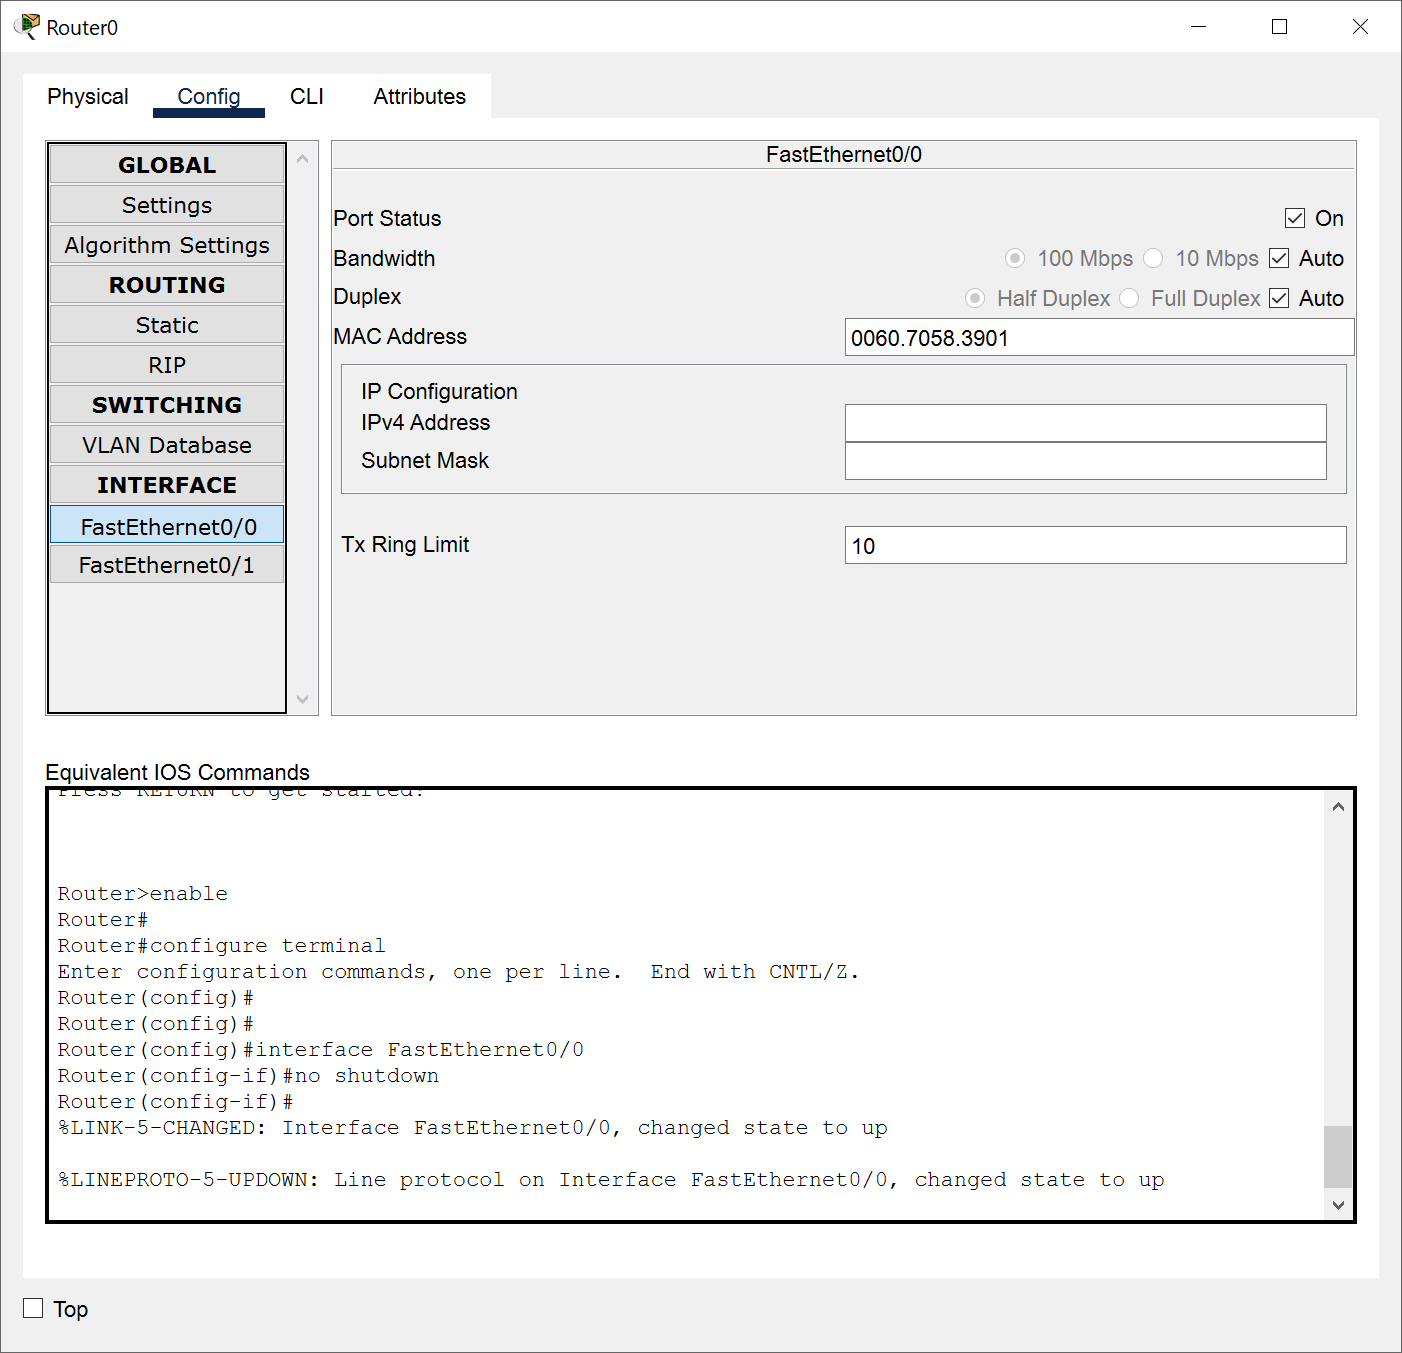
\includegraphics[width=13cm]{./step-by-step/14.PNG}
\clearpage

\noindent as a result of ticking that box now you can see the link going green wich means is enabled for data transmission \newline

\noindent 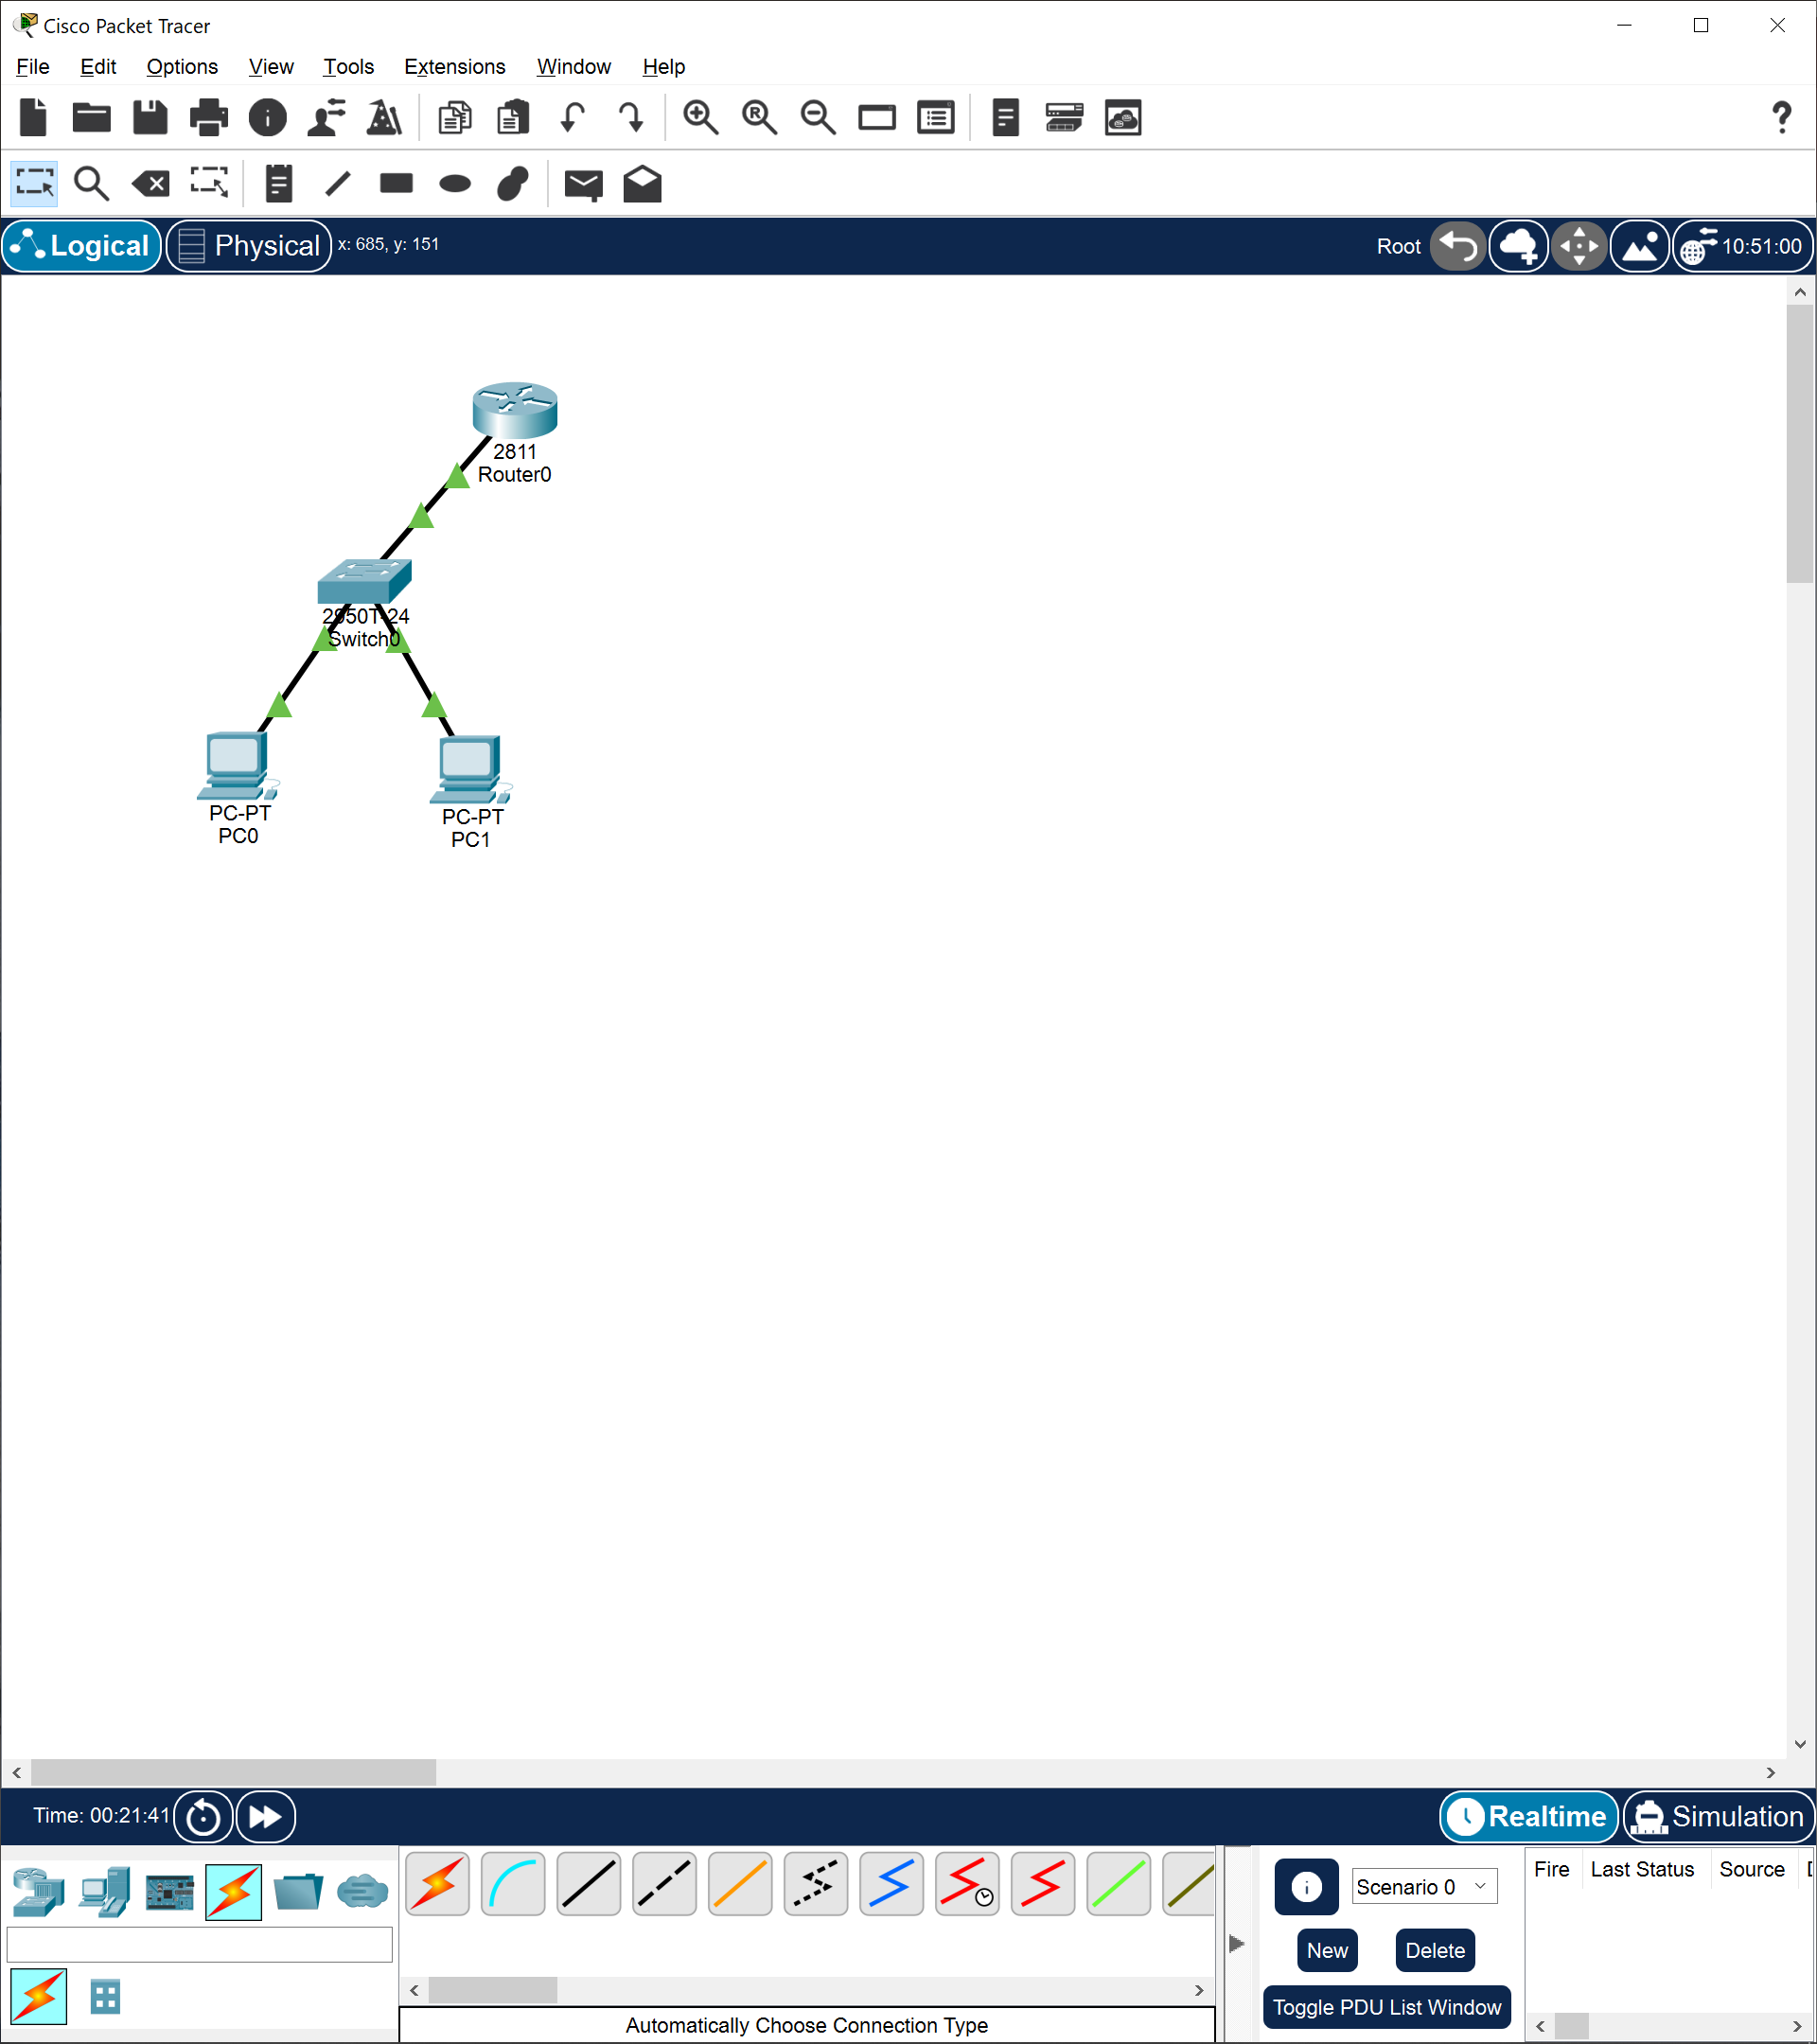
\includegraphics[width=13cm]{./step-by-step/15.PNG}
\clearpage


\noindent we only need to sort the \textbf{IP Configuration} out as well \newline

\noindent 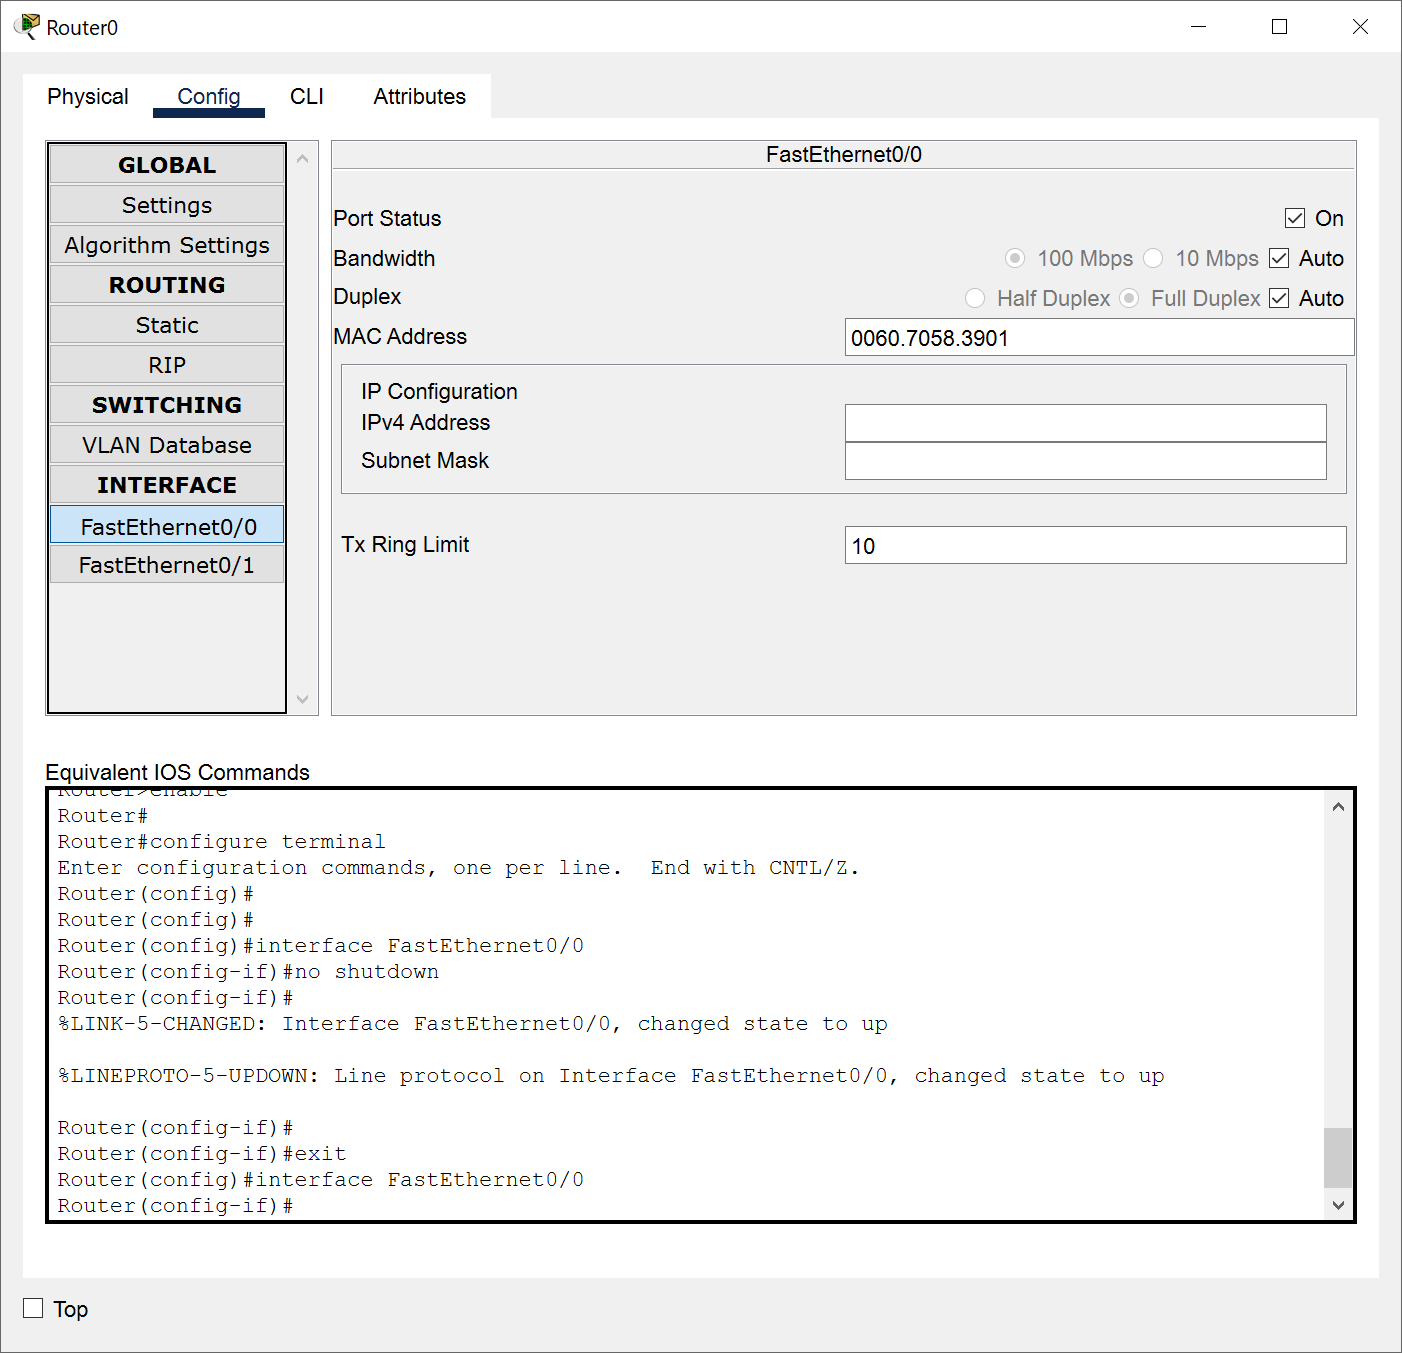
\includegraphics[width=13cm]{./step-by-step/16.PNG}
\clearpage


\noindent Now, because the subnet mask indicates how many values can you actually use this means we can use

\[ 255 values - X values \]

\noindent where \emph{X} is the number in a subnetmask like \emph{Z.Y.W.X} which in the case of \emph{255.255.255.0} will be

\[ 255 - 0\]

\noindent which returns 255 values but because we start counting from 0 we can go up to 254.
In the following example you can see the value 0 being accepted as a valid value \newline 

\noindent 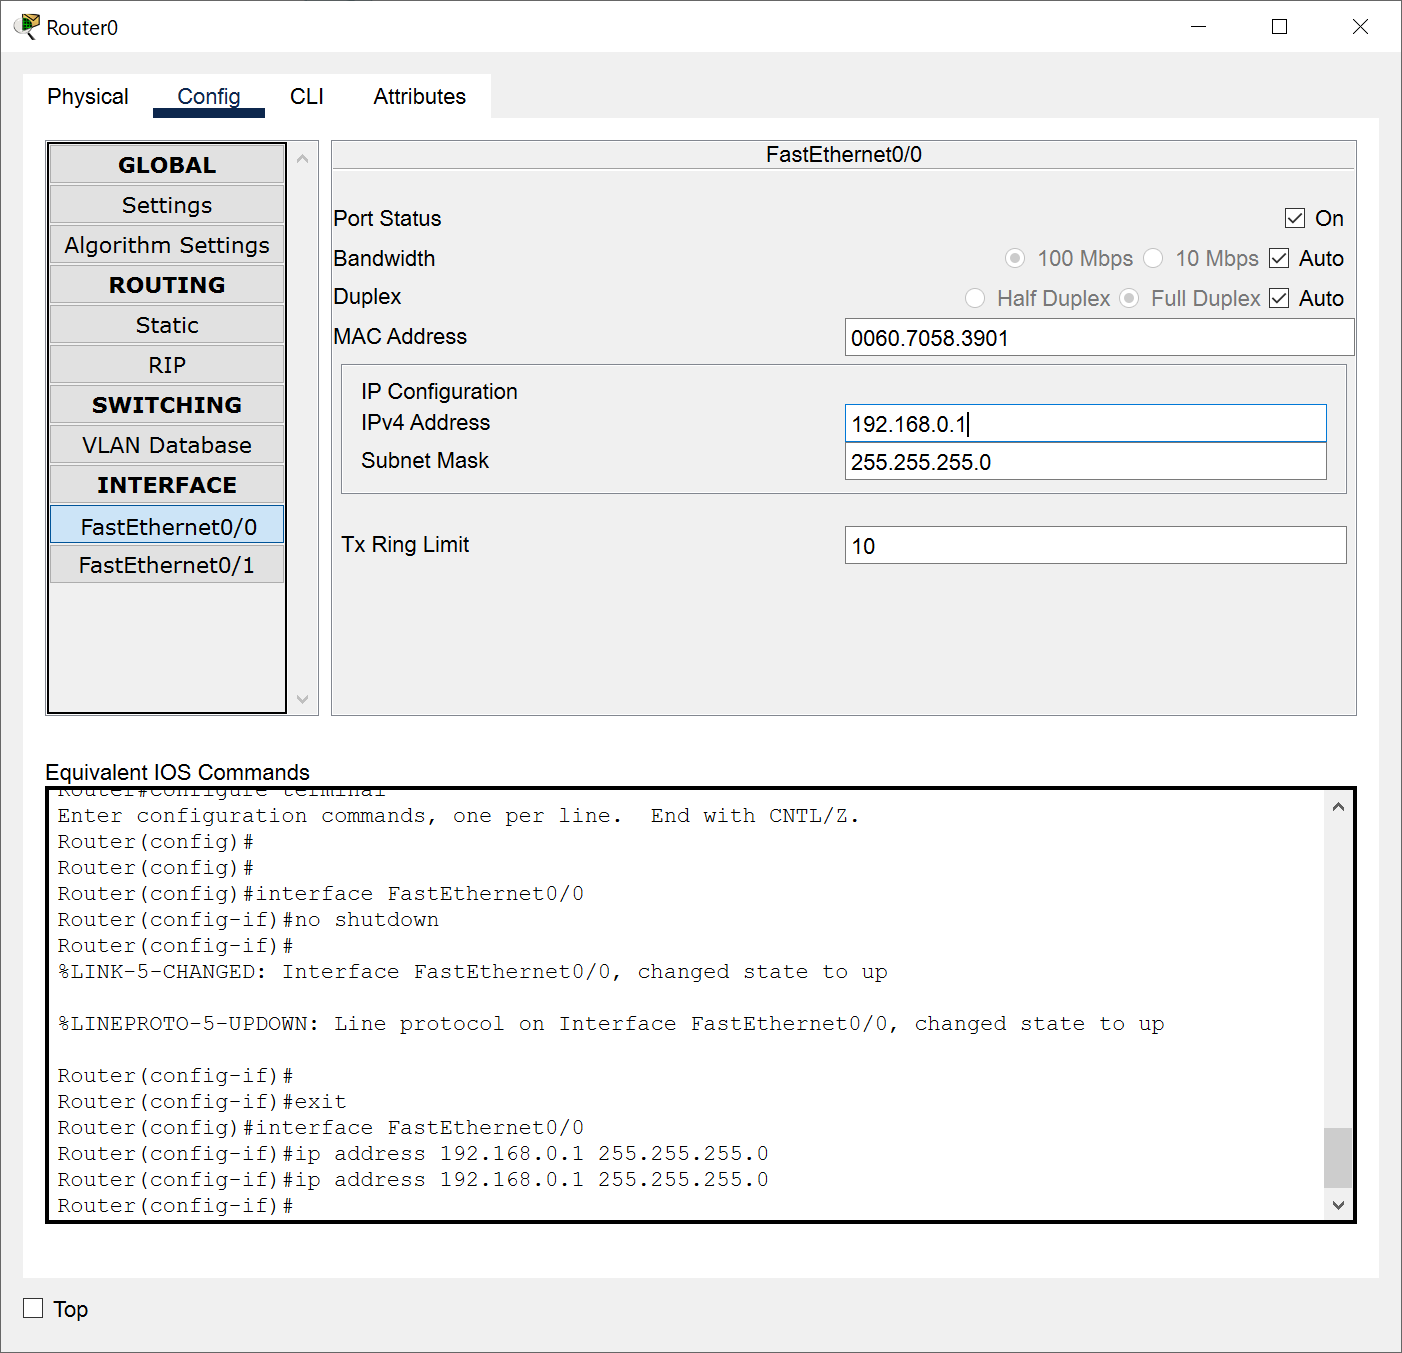
\includegraphics[width=13cm]{./step-by-step/17.PNG}
\clearpage


\noindent Let's pick up PC1 console and ping all devices in the 192.168.0.1 network. The ping works \newline

\noindent 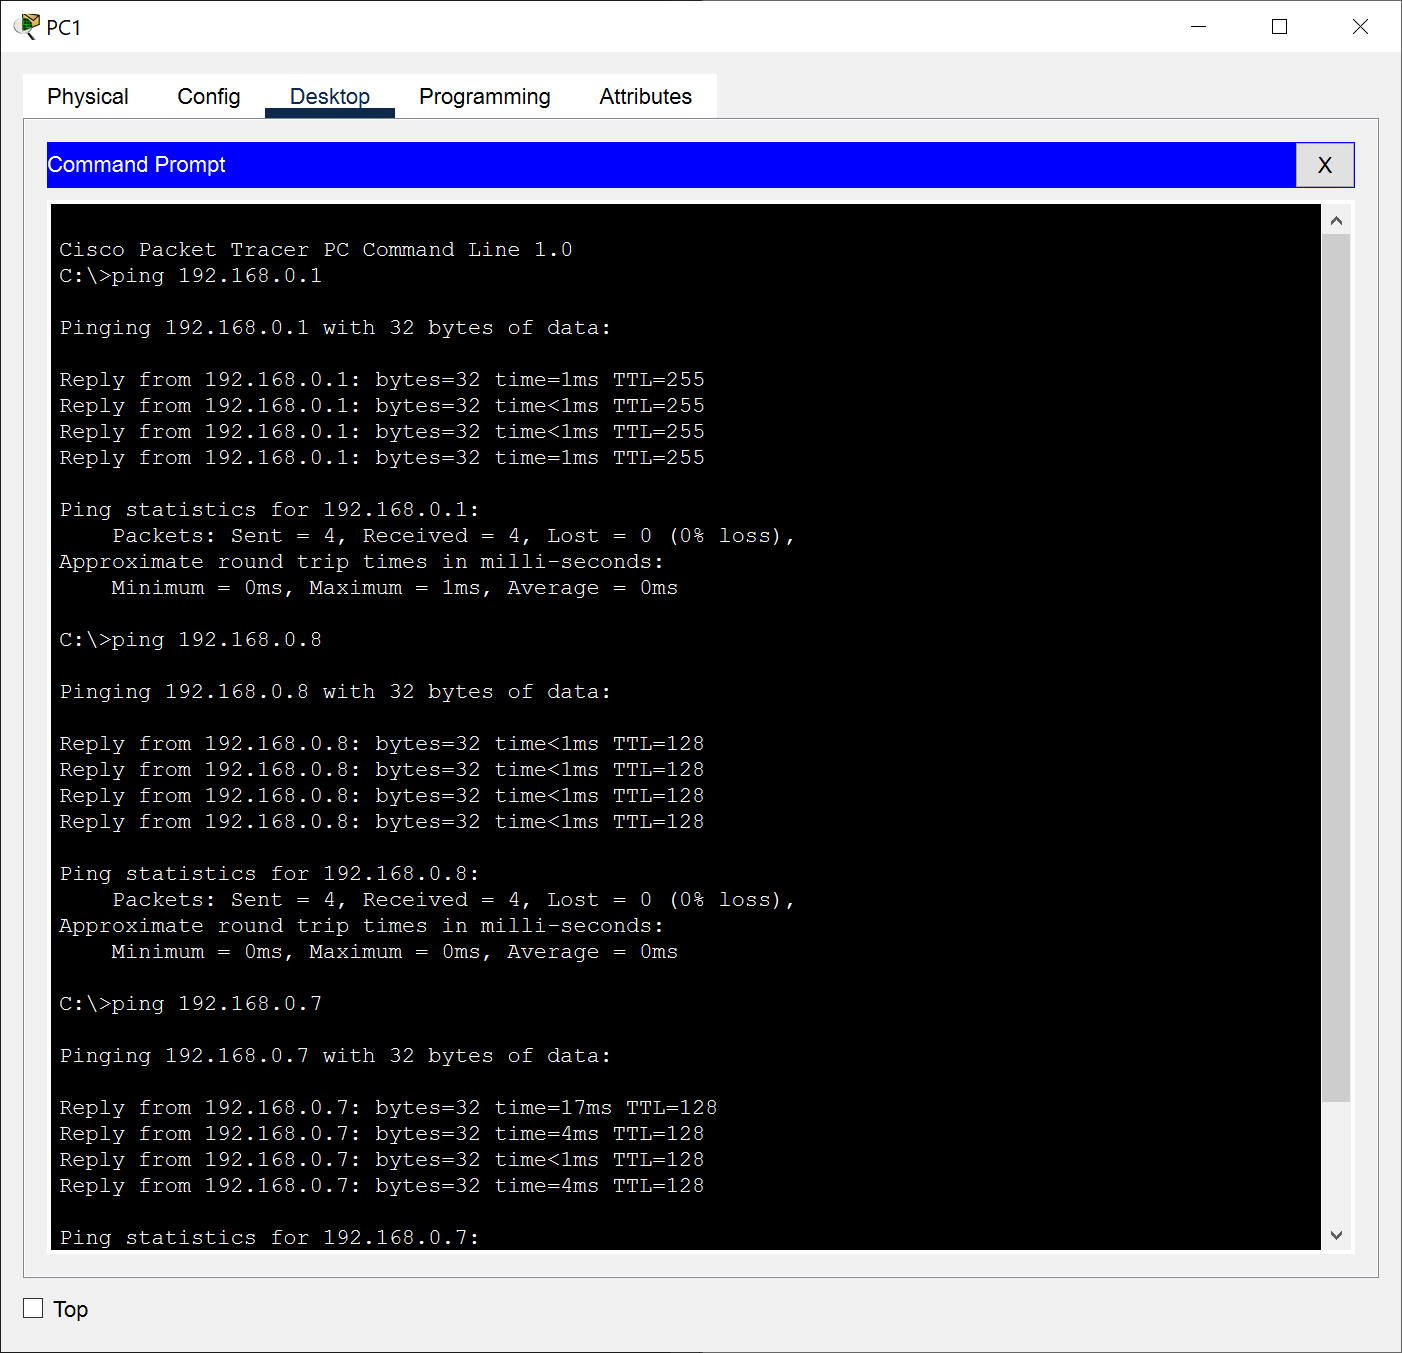
\includegraphics[width=13cm]{./step-by-step/18.PNG}
\clearpage

\noindent Let's create a copy of the subnetwork we have already. The gateway will be this time 
\[192.168.1.1\] \newline
 
\noindent 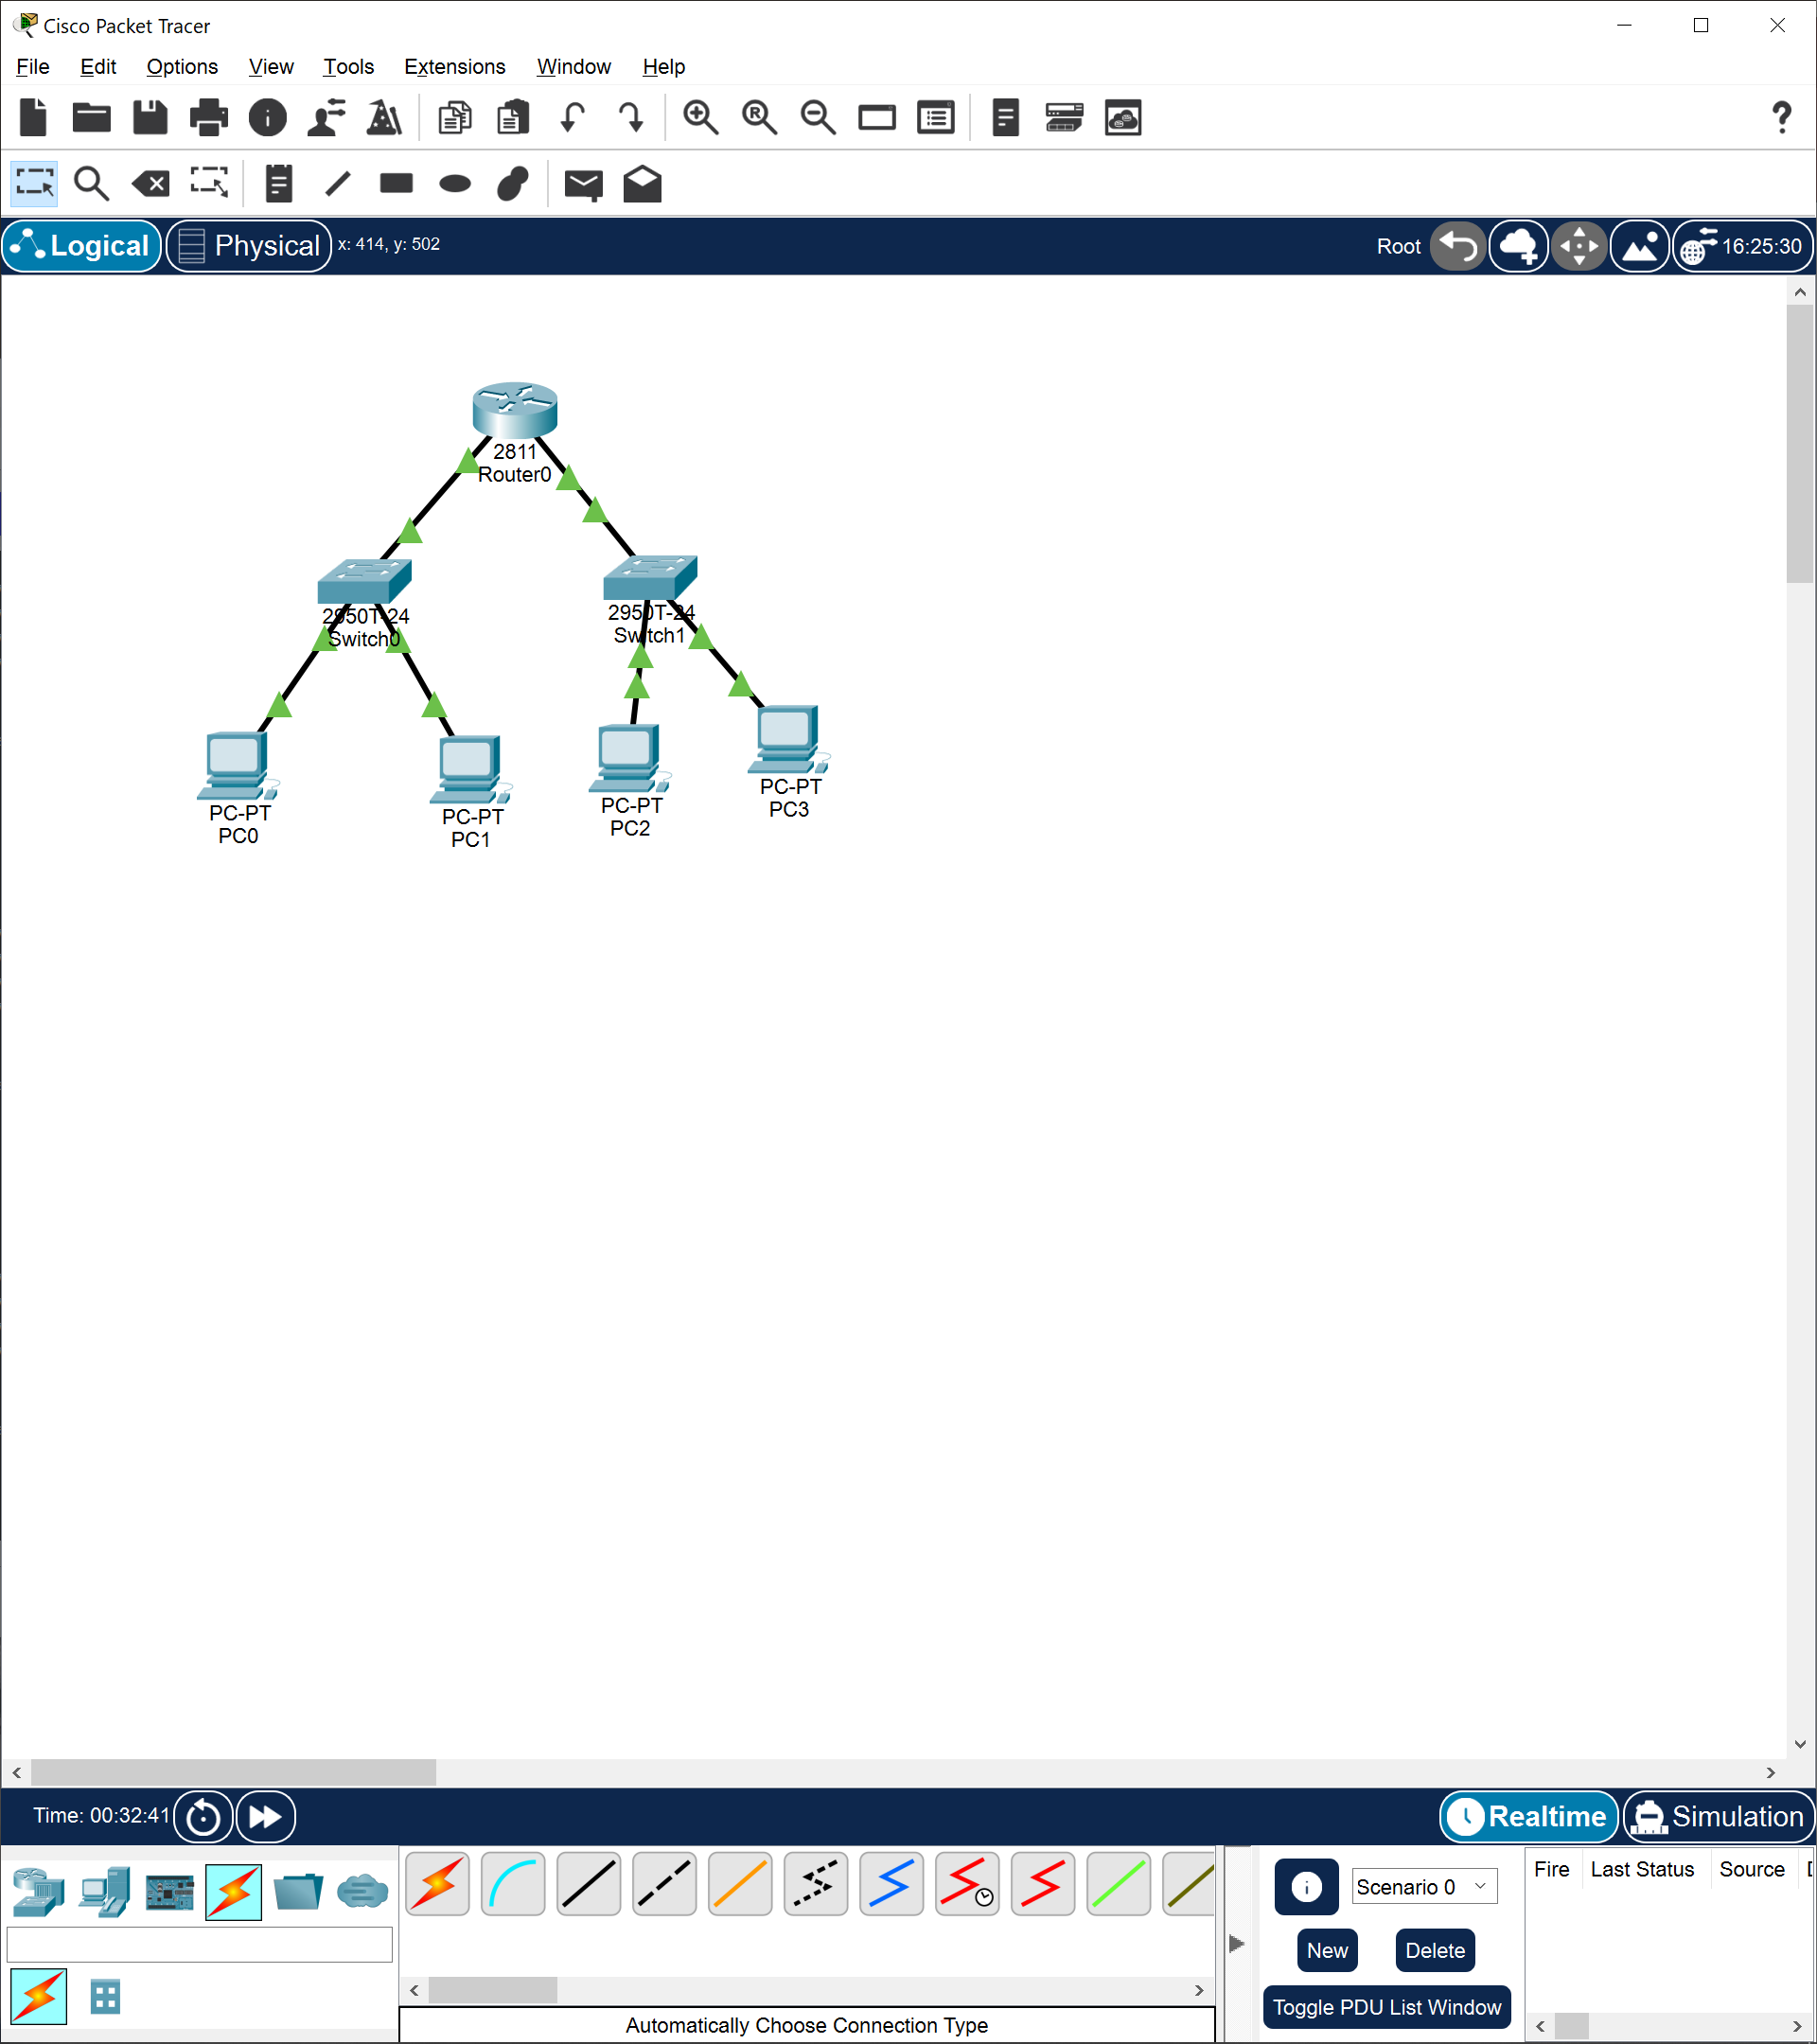
\includegraphics[width=13cm]{./step-by-step/19.PNG}
\clearpage

\subsubsection{expanding the network}
\noindent Let's add a printer with the following IP
\[192.168.1.20\] \newline

\noindent 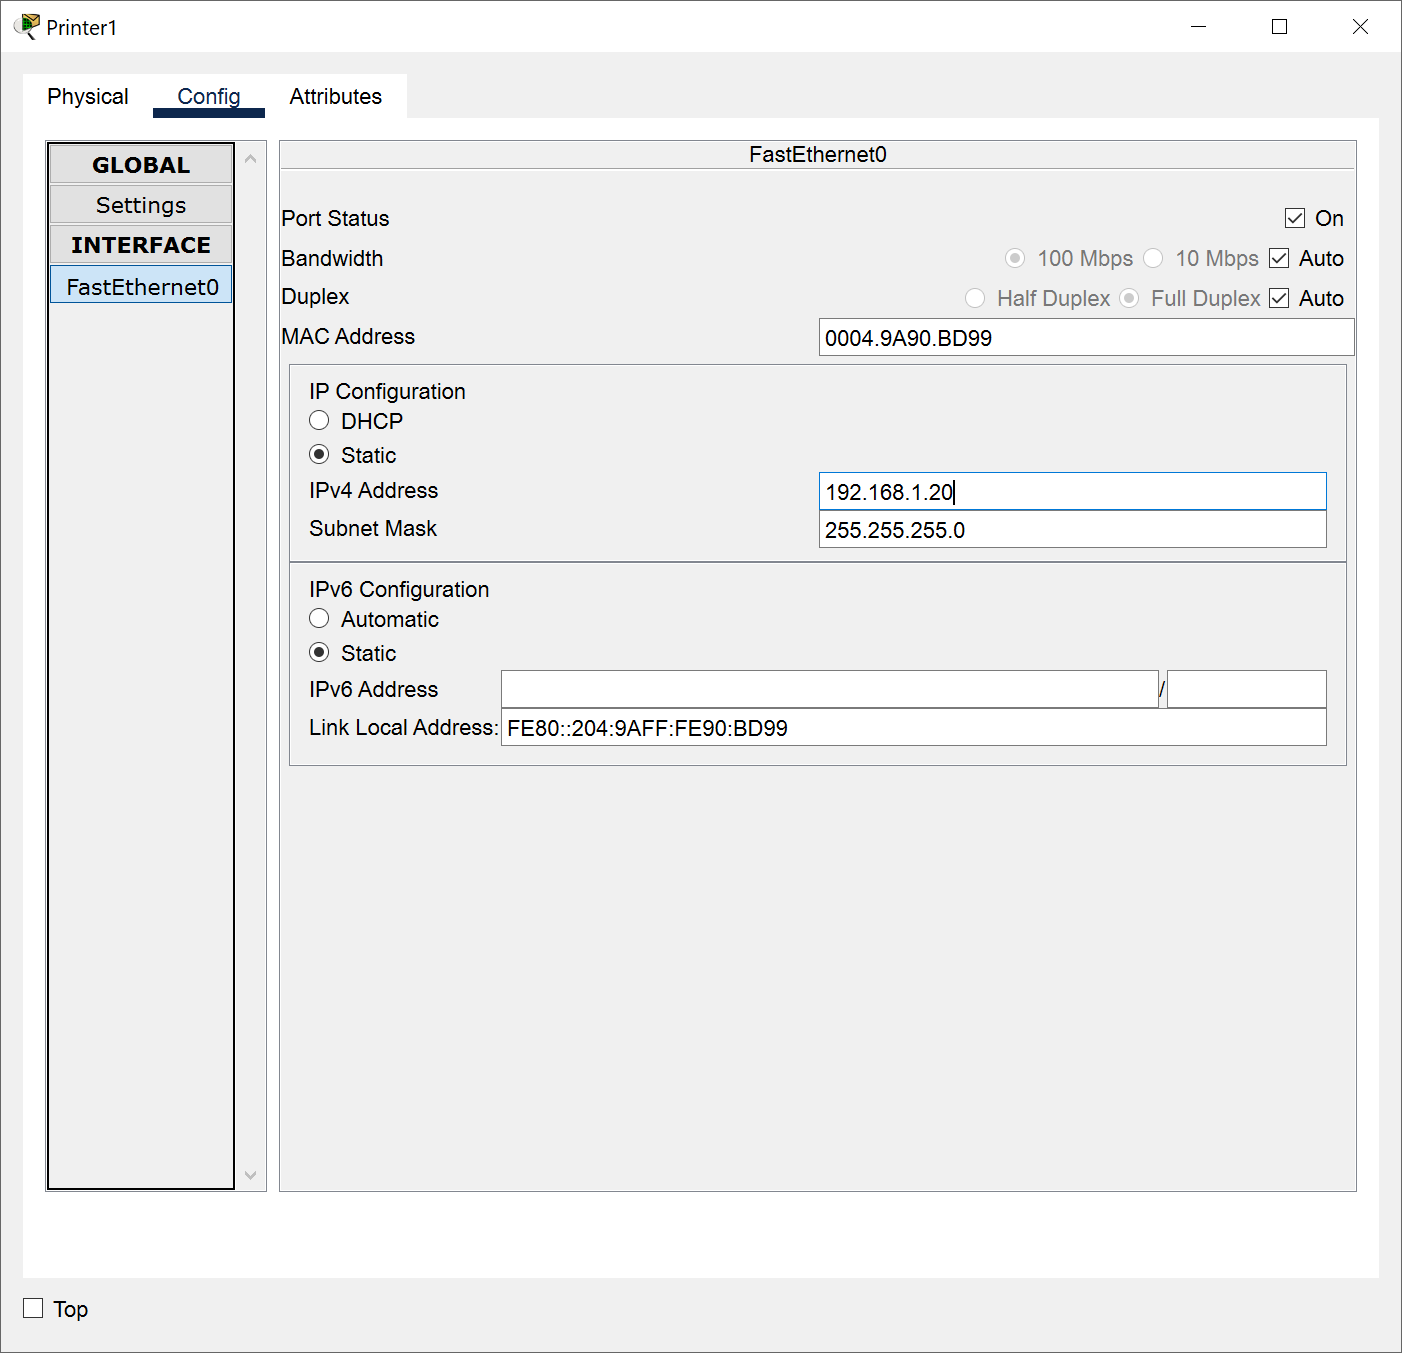
\includegraphics[width=13cm]{./step-by-step/20.PNG}
\clearpage

\noindent Let's ping the printer from PC0\newline

\noindent 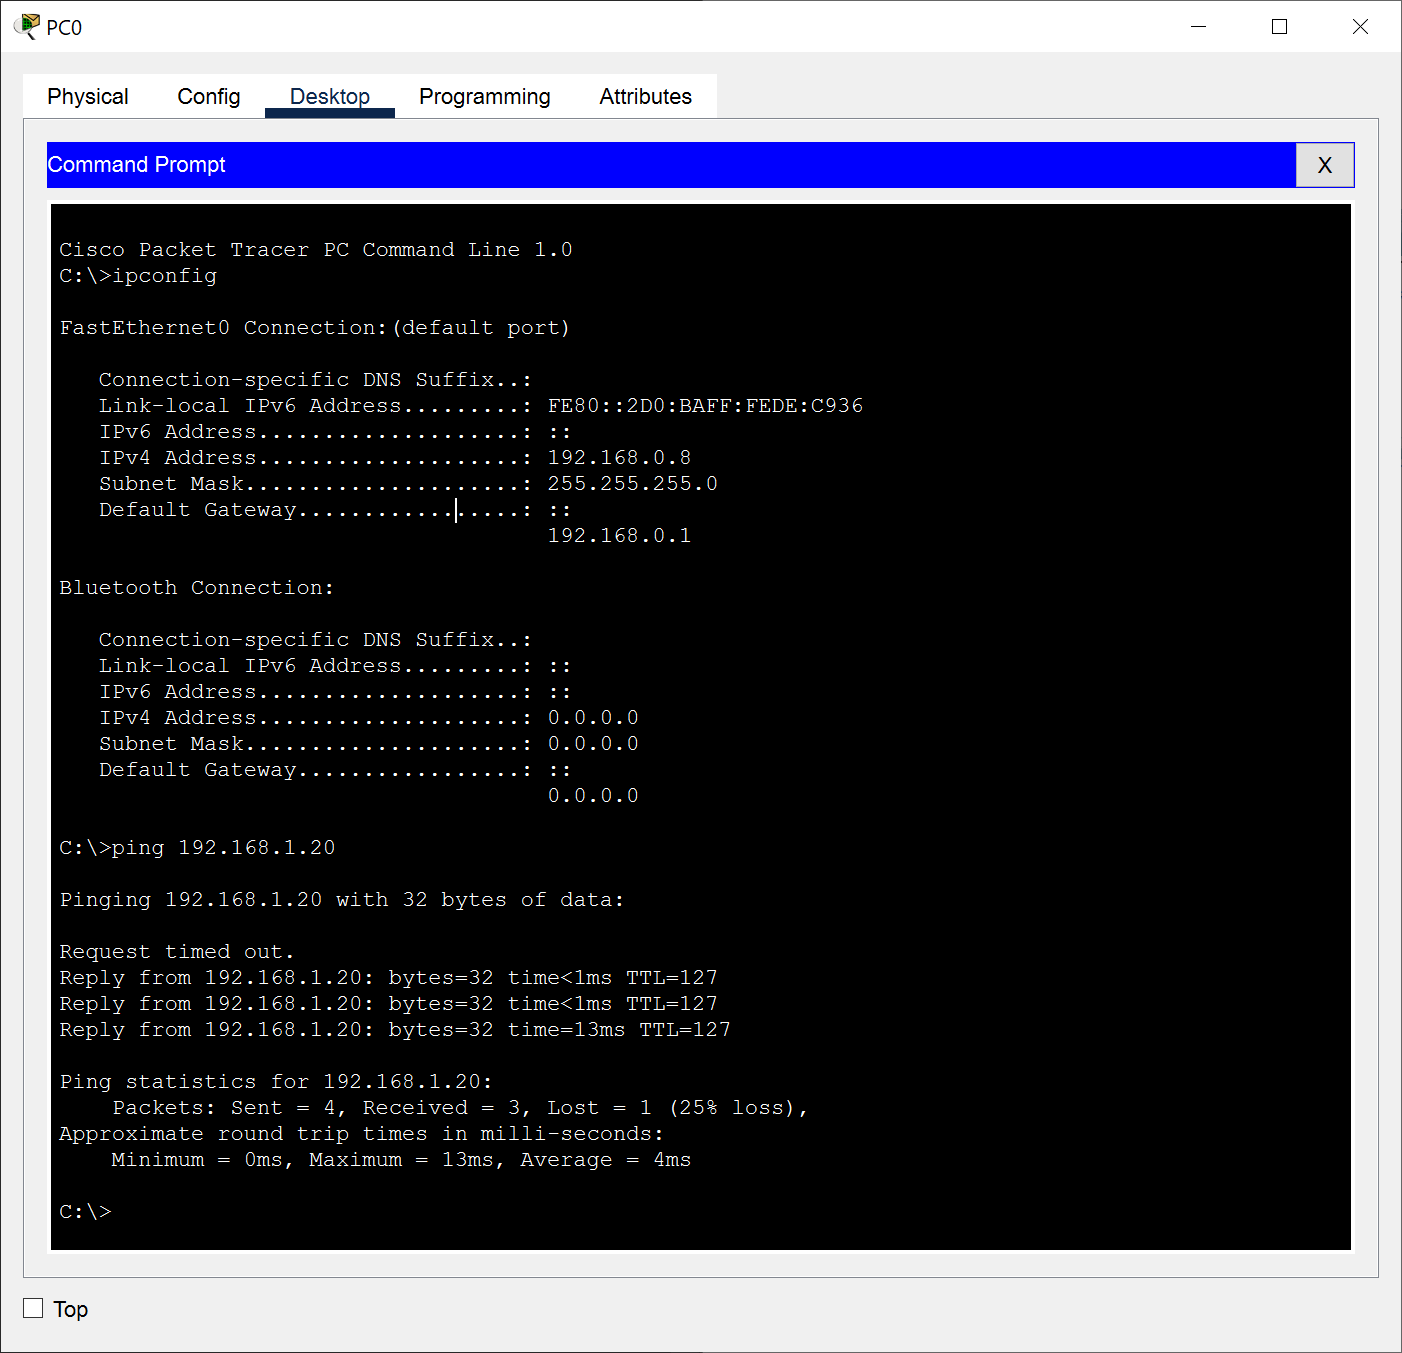
\includegraphics[width=13cm]{./step-by-step/21.PNG} \newline
\noindent We can safely assume the network is working
\clearpage



\section{Power over Ethernet}
Power over Ethernet is a technique for delivering DC power to devices over copper Ethernet cabling, eliminating the need for separate power supplies and outlets. While PoE doesn't add Ethernet data capabilities, it does offer expanded options for how and where Ethernet end devices can be placed.

%\section{LAN status LEDs}

\section{Network Topology}

Network topology is the arrangement of the elements (links, nodes, etc.) of a communication network.

Network topology is the structure of a network and may be depicted physically or logically. It is an application of graph theory wherein communicating devices are modeled as nodes and the connections between the devices are modeled as links or lines between the nodes. Physical topology is the placement of the various components of a network (e.g., device location and cable installation), while logical topology illustrates how data flows within a network. Distances between nodes, physical interconnections, transmission rates, or signal types may differ between two different networks, yet their logical topologies may be identical. A network’s physical topology is a particular concern of the physical layer of the OSI model.

Examples of network topologies are found in local area networks (LAN), a common computer network installation. Any given node in the LAN has one or more physical links to other devices in the network; graphically mapping these links results in a geometric shape that can be used to describe the physical topology of the network. A wide variety of physical topologies have been used in LANs, including ring, bus, mesh and star. Conversely, mapping the data flow between the components determines the logical topology of the network. In comparison, Controller Area Networks, common in vehicles, are primarily distributed control system networks of one or more controllers interconnected with sensors and actuators over, invariably, a physical bus topology.
\clearpage

\subsection{Star Topology}

In star topology, every peripheral node (computer workstation or any other peripheral) is connected to a central node called a hub or switch. The hub is the server and the peripherals are the clients. The network does not necessarily have to resemble a star to be classified as a star network, but all of the peripheral nodes on the network must be connected to one central hub. All traffic that traverses the network passes through the central hub, which acts as a signal repeater.

\noindent 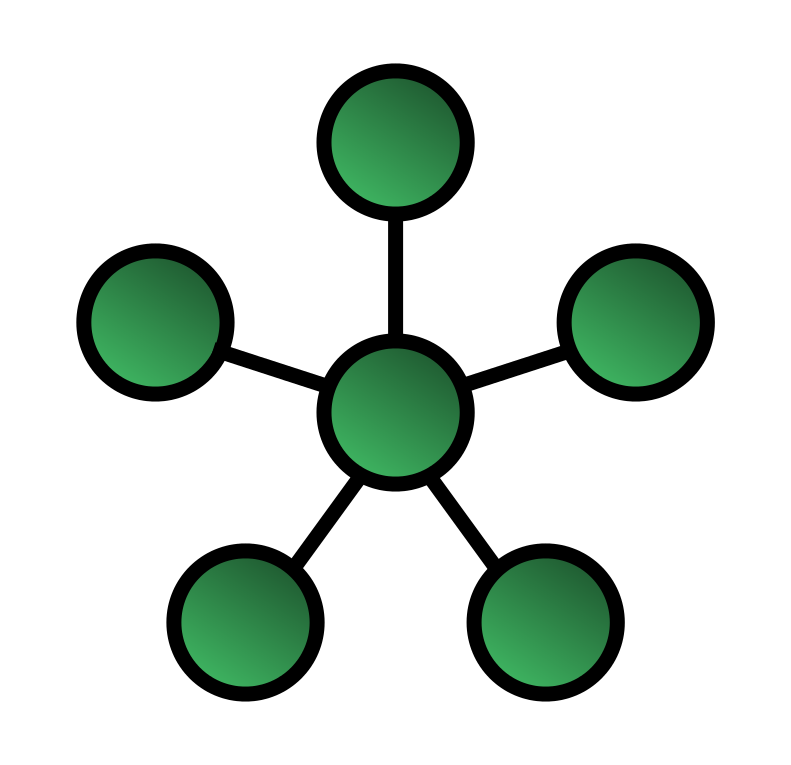
\includegraphics[width=7cm]{./StarNetwork.svg.PNG} \newline

\subsubsection{PROs}

\begin{itemize}
\item {simplicity of adding additional nodes}
\item {is the easiest topology to design and implement}
\end{itemize}

\subsubsection{CONs}

\begin{itemize}
\item {the hub represents a single point of failure}
\item {Since all peripheral communication must flow through the central hub, the aggregate central bandwidth forms a network bottleneck for large clusters}
\end{itemize}

\clearpage

\subsection{Ring Topology}

A ring topology is a daisy chain in a closed loop. Data travels around the ring in one direction. When one node sends data to another, the data passes through each intermediate node on the ring until it reaches its destination. The intermediate nodes repeat (re transmit) the data to keep the signal strong.\footnotemark{} Every node is a peer; there is no hierarchical relationship of clients and servers. If one node is unable to re transmit data, it severs communication between the nodes before and after it in the bus.

\noindent 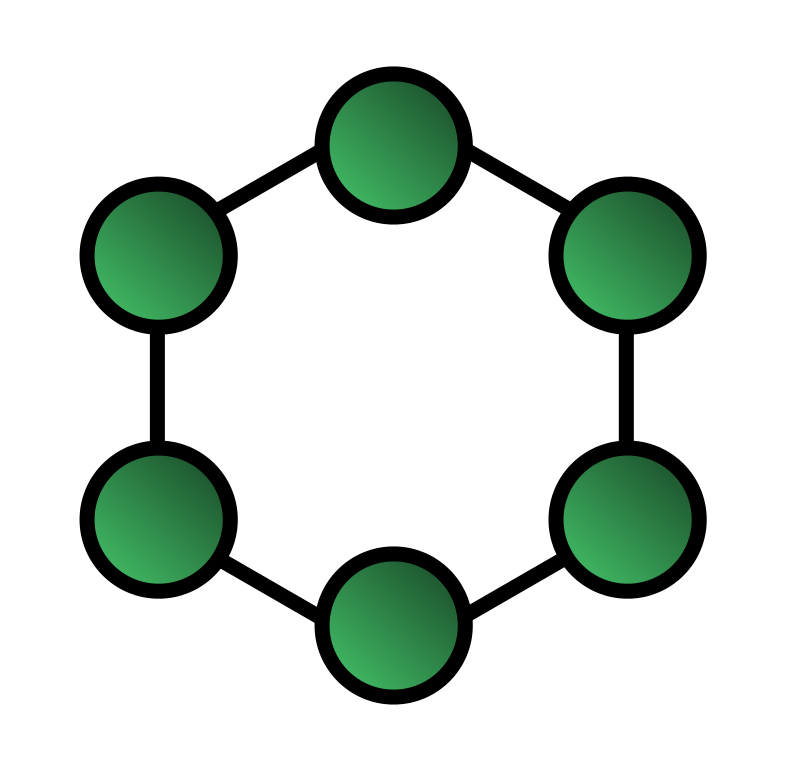
\includegraphics[width=7cm]{./RingNetwork.svg.PNG} \newline
\footnotetext{ Inc, S., (2002) . Networking Complete. Third Edition. San Francisco: Sybex }

\subsubsection{PROs}

\begin{itemize}
\item {When the load on the network increases, its performance is better than bus topology}
\item {There is no need of network server to control the connectivity between workstations}
\end{itemize}

\subsubsection{CONs}

\begin{itemize}
\item {Aggregate network bandwidth is bottlenecked by the weakest link between two nodes}
\end{itemize}

\clearpage
\subsection{Ring Topology on Cisco Packet Tracer}

This is a quick example of how can a Ring Topology look like on Cisco Packet Tracer. The links at the center have been added later on for testing purporses

\noindent 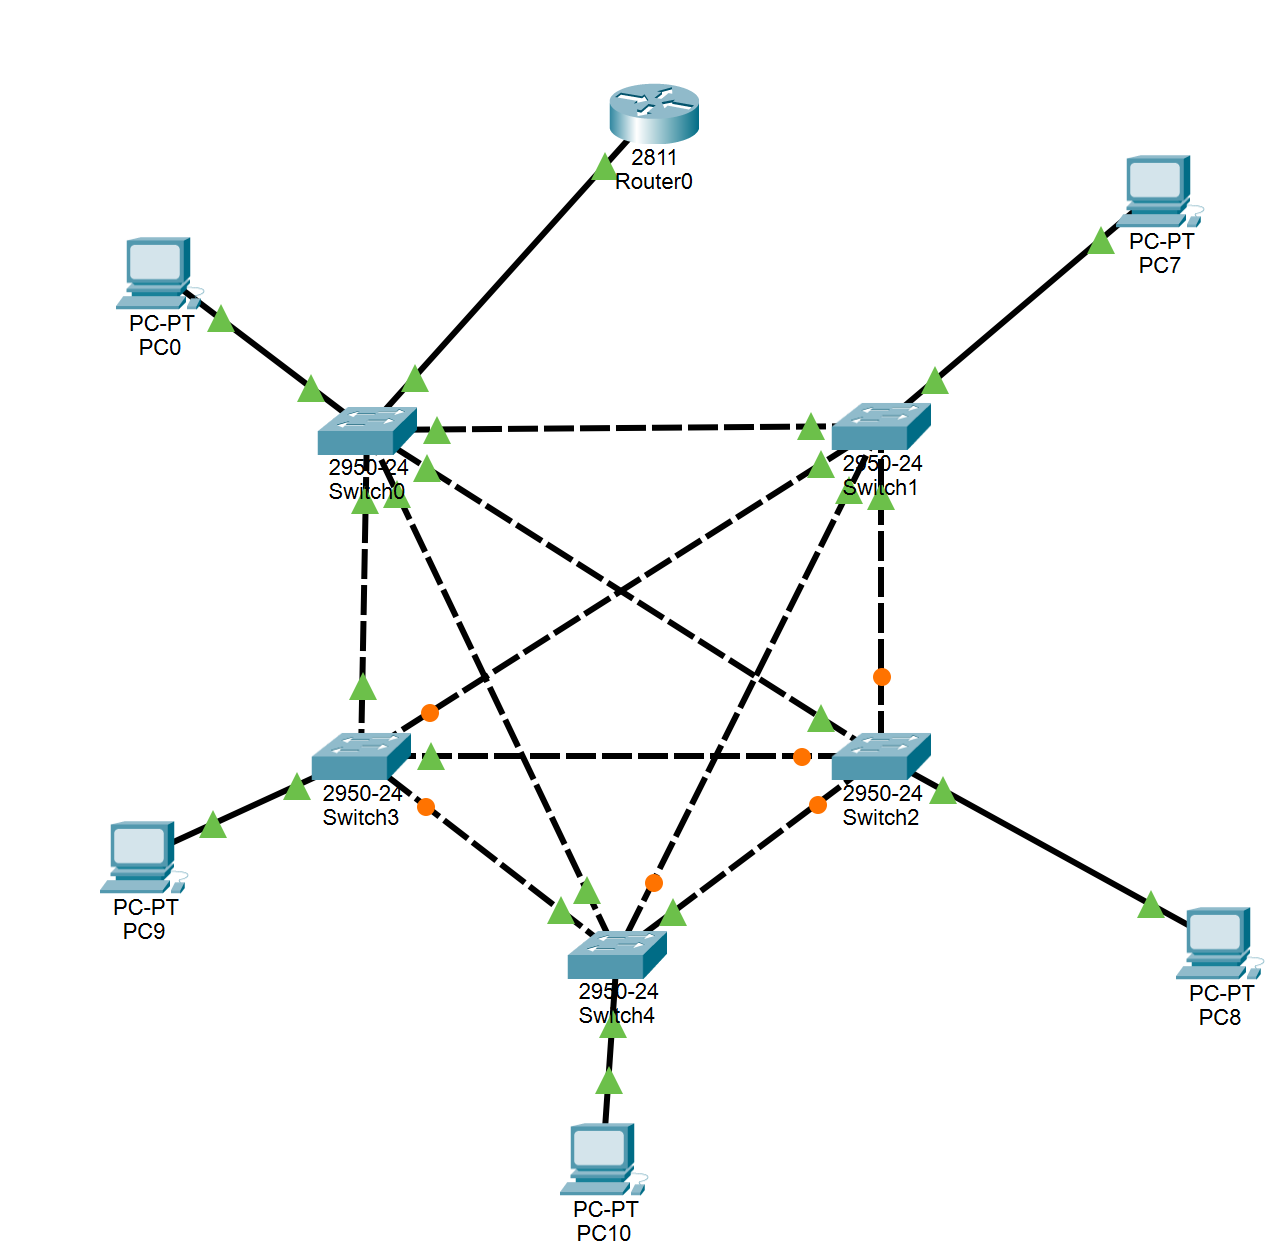
\includegraphics[width=7cm]{./star-topology/screenshot.PNG} \newline

\section{Routing Protocols}

A routing protocol specifies how routers communicate with each other to distribute information that enables them to select routes between nodes on a computer network. Routers perform the traffic directing functions on the Internet; data packets are forwarded through the networks of the internet from router to router until they reach their destination computer. Routing algorithms determine the specific choice of route. Each router has a prior knowledge only of networks attached to it directly. A routing protocol shares this information first among immediate neighbors, and then throughout the network. This way, routers gain knowledge of the topology of the network. The ability of routing protocols to dynamically adjust to changing conditions such as disabled connections and components and route data around obstructions is what gives the Internet its fault tolerance and high availability. \newline

The specific characteristics of routing protocols include the manner in which they avoid routing loops, the manner in which they select preferred routes, using information about hop costs, the time they require to reach routing convergence, their scalability, and other factors such as relay multiplexing and cloud access framework parameters. Certain additional characteristics such as multilayer interfacing may also be employed as a means of distributing uncompromised networking gateways to authorized ports. This has the added benefit of preventing issues with routing protocol loops.

Many routing protocols are defined in technical standards documents called RFCs

\section{Interior gateway protocols}
An interior gateway protocol (IGP) is a type of routing protocol used for exchanging routing table information between gateways (commonly routers) within an \textbf{autonomous system} \footnote{\label{autonomous-system}for example, a system of corporate local area networks}. This routing information can then be used to route network-layer protocols like IP.

Interior gateway protocols can be divided into two categories: \textbf{distance-vector} routing protocols and \textbf{link-state} routing protocols.

\subsection{link state routing protocols}
\textbf{Link-state} routing protocols are one of the two main classes of routing protocols used in packet switching networks for computer communications, the other being \textbf{distance-vector} routing protocols. One example of link-state routing protocols is Open Shortest Path First (OSPF).% and Intermediate System to Intermediate System (IS-IS).

The link-state protocol is performed by every switching node in the network (i.e., nodes that are prepared to forward packets; in the Internet, these are called routers). The basic concept of link-state routing is that every node constructs a map of the connectivity to the network, in the form of a graph, showing which nodes are connected to which other nodes. Each node then independently calculates the next best logical path from it to every possible destination in the network. Each collection of best paths will then form each node's routing table.

This contrasts with distance-vector routing protocols, which work by having each node share its routing table with its neighbours. %in a link-state protocol the only information passed between nodes is connectivity related.% Link-state algorithms are sometimes characterized informally as each router, "telling the world about its neighbors."

\subsubsection{OSPF}
Open Shortest Path First (OSPF) is a routing protocol for Internet Protocol (IP) networks. It uses a link state routing (LSR) algorithm and falls into the group of interior gateway protocols (IGPs) \textsc{\textbf{meaning it is}} operating within a single autonomous system.

OSPF gathers link state information from available routers and constructs a topology map of the network. The topology is presented as a routing table to the Internet Layer for routing packets by their destination IP address. 

%OSPF supports Internet Protocol Version 4 (IPv4) and Internet Protocol Version 6 (IPv6) networks and supports the Classless Inter-Domain Routing (CIDR) addressing model.
%
%OSPF is widely used in large enterprise networks. IS-IS, another LSR-based protocol, is more common in large service provider networks.

%Originally designed in the 1980s, OSPF is defined for IPv4 in protocol version 2 by RFC 2328 (1998).[1] The updates for IPv6 are specified as OSPF Version 3 in RFC 5340 (2008).OSPF supports the Classless Inter-Domain Routing (CIDR) addressing model.

\subsection{distance vector routing protocols}
A distance-vector routing protocol in data networks determines the best route for data packets based on distance. Distance-vector routing protocols measure the distance by the number of routers a packet has to pass; one router counts as one hop. Some distance-vector protocols also take into account network latency and other factors that influence traffic on a given route. To determine the best route across a network, routers using a distance-vector protocol exchange information with one another, usually routing tables plus hop counts for destination networks and possibly other traffic information. Distance-vector routing protocols also require that a router inform its neighbours of network topology changes periodically.

Distance-vector routing protocols use the Bellman–Ford algorithm to calculate the best route. Another way of calculating the best route across a network is based on link cost, and is implemented through link-state routing protocols.

The term distance vector refers to the fact that the protocol manipulates vectors (arrays) of distances to other nodes in the network. The distance vector algorithm was the original ARPANET routing algorithm and was implemented more widely in local area networks with the Routing Information Protocol (RIP).

\subsubsection{RIP}
The Routing Information Protocol (RIP) is one of the oldest distance-vector routing protocols which employs the hop count as a routing metric. RIP prevents routing loops by implementing a limit on the number of hops allowed in a path from source to destination. The largest number of hops allowed for RIP is 15, which limits the size of networks that RIP can support.

RIP implements the split horizon, route poisoning, and holddown mechanisms to prevent incorrect routing information from being propagated.

In RIPv1 routers broadcast updates with their routing table every 30 seconds. In the early deployments, routing tables were small enough that the traffic was not significant. As networks grew in size, however, it became evident there could be a massive traffic burst every 30 seconds, even if the routers had been initialized at random times.

It is easy to configure, because RIP does not require any parameters, unlike other protocols.
%RIP uses the UDP as its transport protocol.
%and is assigned the reserved port number 520.
\subsubsection{EIGRP}
Enhanced Interior Gateway Routing Protocol (EIGRP) is an advanced distance-vector routing protocol that is used on a computer network for automating routing decisions and configuration.EIGRP is used on a router to share routes with other routers within the same autonomous system. Unlike other well known routing protocols, such as RIP, EIGRP only sends incremental updates, reducing the workload on the router and the amount of data that needs to be transmitted.EIGRP replaced the Interior Gateway Routing Protocol (IGRP) because this one didn't support classless IPv4 addresses.

\section{Exterior gateway protocols}

An exterior gateway protocol is a routing protocol used to exchange routing information between autonomous systems. This exchange is crucial for communications across the Internet. Notable exterior gateway protocols include Exterior Gateway Protocol (EGP), now obsolete, and Border Gateway Protocol (BGP)\footnote{\label{EGP}  Hunt, Craig (2002). \href{http://web.deu.edu.tr/doc/oreily/networking/tcpip/index.htm}{TCP/IP network administration} (3 ed.). O'Reilly Media. ISBN 9781449391430. OCLC 52356435. Archived from the original on 1 July 2020. Retrieved 5 November 2021 – via Dokuz Eylül University.}${}^{{}^{7 \cdot 5}}$:  

\subsection{BGP}
Border Gateway Protocol (BGP) is a standardized exterior gateway protocol designed to exchange routing and reachability information among autonomous systems$ ^{\ref{autonomous-system}}$ on the Internet. BGP is classified as a path-vector routing protocol, and it makes routing decisions based on paths, network policies, or rule-sets configured by a network administrator.

BGP used for routing within an autonomous system is called Interior Border Gateway Protocol, Internal BGP (iBGP). In contrast, the Internet application of the protocol is called Exterior Border Gateway Protocol, External BGP (eBGP).

\section{IoT}
The \textbf{Internet of things} describes physical objects with sensors, processing ability, software, and other technologies that connect and exchange data with other devices and systems over the Internet or other communications networks.Internet of things has been considered a misnomer because devices do not need to be connected to the public internet, they only need to be connected to a network and be individually addressable.

\section{IoT in Aviation}
With the inclusion of digital technologies, the airline industry has now been able to deliver unique customer experiences, simplified underlying processes, and most importantly enhancing the productivity of the workforce. The next stride in leveraging IoT can lead to the exploration of newer dimensions in the aviation industry. Combining IoT with other technologies like AI and robotics would generate a number of opportunities related to service delivery improvement. Further, a smart  IoT ecosystem can bring in all the required entities and assets together in the industry value chain and make it look like the new normal.

\subsection{Existing Technologies in Aviation Industry}
\subsubsection{Digitized Security}
Today, state-of-the-art technology is being developed for implementing advanced concepts such as “walk through security” to reduce the passenger waiting times. Biometrics are also being used for automating the verification processes, thus reducing the burden of staffing.

Security systems are increasingly becoming a major technology trend at the airport terminals as these are equipped with the latest security system for security purposes.

\subsubsection{VR for Last-Minute Changes}
A leading global aviation company has been testing a new way for its passengers to upgrade their tickets by allowing them premium seats using VR. The airline company allows passengers to upgrade at the last  minute. The airline company said that the best way for understanding the benefits of a premium economy, that has extra legroom and seat pitch can be done virtualized using VR.

\subsubsection{Biometrics}
Biometrics are being potentially used by the aviation industry for some time now and is gaining a stronghold across this industry vertical. Some of the biggest airports across the world have invested in fingerprint and facial recognition technology. The aviation industry emphasizes on using facial recognition so that the passenger’s face becomes the new passport. Also at various airports, biometric-based recognition is being implemented at the airport lounge entrance and integrating this technology with flight information display systems for serving the passengers with a higher degree of personalized information along with offers.

\subsection{IoT Adoption Challenges}

\textbf{Following are some key challenges that are to be addressed for implementing IoT on a wide scale. These are inclusive of -}

\begin{itemize}
\item{ Most of the airline companies operate on a global level spread across diversified geographical boundaries. Each of these geographies has its own cultural diversity as well as technological adaptability. A successfully implemented IoT needs to support these regional variations.}
\item{ The airline industry operates in a top-notched secure environment. Thus, security and privacy need to be the top priority for implementing IoT in the aviation industry. Privacy can also be seen as a critical issue whenever there is a deployment of advanced technologies such as facial recognition as an outcome of the large volume of passenger’s private data.}
\end{itemize}

\subsection{Opportunities for IoT in Aviation}

IoT offers a number of tremendous benefits to the aviation industry and its rippling effects include- reduced travel times, enhancing the comfort levels of passengers with better security levels. In order to fully realize the \textbf{IoT} opportunities, the businesses and governments need to coordinate with the same frequency for answering the political as well as business issues related to IoT.

\noindent \textbf{This disruptive technology holds several benefits when it comes to the aviation industry -}

\begin{itemize}
\item{ When sensors are embedded in connected objects, it can be used for controlling, monitoring and collecting accurate real-time data. Sensors have significantly improved over the past few years. Wireless can be a key driver behind the emergence of IoT devices that operate on Wi-Fi or a strong cellular network such as 5G. Using a low-power wide area network (LPWAN) could be used for enriching the performance of sensors that offer low bandwidth.}
\item{ Cloud Computing can be used for creating a common platform for handling and integrating data from several sources like- people, their processes and their systems (devices). Real-time data can be utilized for gaining purposeful insights from current market data ad then distribute this information to the customers in a very short span of time.}
\item{ The airport terminals can duplicate the underlying concept of \textbf{smart cities}, thereby, implementing advanced technologies besides improved methods for collecting data to mine out the meaningful real-time insights. The use of sensor data could be done for improving operations and cumulative passenger experience. Multiple data sets can be integrated, optimized and analyzed for developing smarter applications and services related to airports, aircraft, and passengers.}
\item{ Beacons offer tremendous scope for IoT gateways. These can be placed across the entire airport infrastructure for triggering notifications on the passenger’s mobile as soon as he is in the beacon’s range. These notifications could be related to time, flight status or even displaying an e-boarding pass on the passenger’s mobile. This, in turn, provides the passenger with more accurate information every time. This can even help the airline crew for determining how far is the passenger from the airline in order to determine how long they need to wait before the actual take-off.}
\end{itemize}

\section{IPv6}

Internet Protocol version 6 (IPv6) is the most recent version of the Internet Protocol (IP), the communications protocol that provides an identification and location system for computers on networks and routes traffic across the Internet. IPv6 was developed by the Internet Engineering Task Force (IETF) to deal with the long-anticipated problem of IPv4 address exhaustion, and is intended to replace IPv4\footnotemark{}.

\clearpage

\begin{wrapfigure}{3cm}
\centering
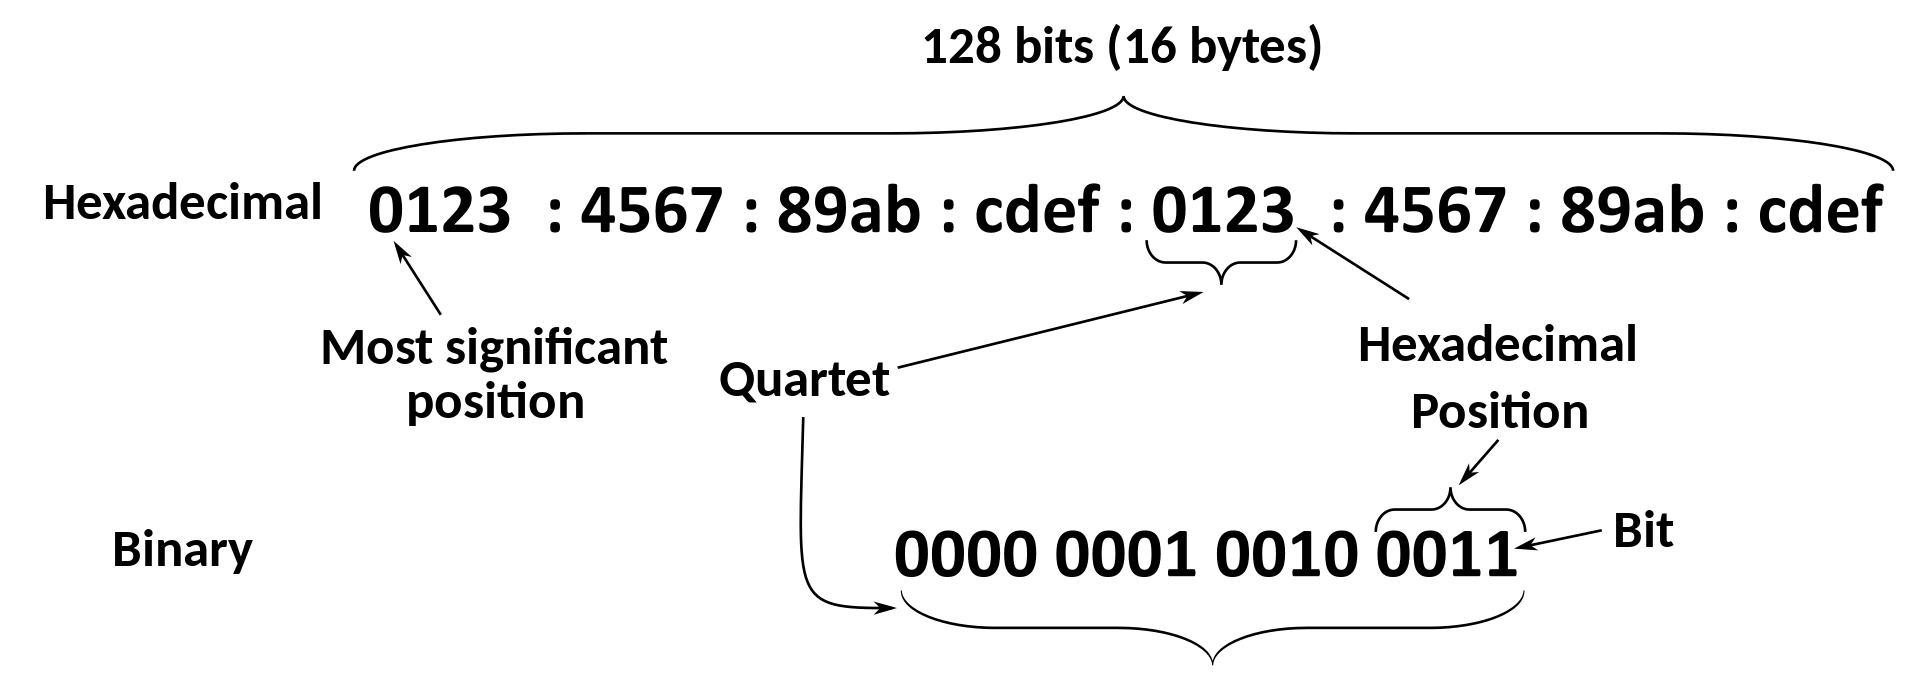
\includegraphics[width=10cm]{./IPv6.PNG}
%\vspace{-10pt}
\caption{IPv6 8-bytes Format }\label{wrap-fig:7}
\end{wrapfigure}

\footnotetext{ "FAQs". New Zealand IPv6 Task Force. Archived from the original on 29 January 2019. Retrieved 26 October 2015.}

\subsection{IPsec}
Internet Protocol Security (IPsec) was originally developed for IPv6, but found widespread deployment first in IPv4, for which it was re-engineered, however, IPv4 doesn't include it automatically whereas with IPv6 it will be mandatory.

\subsubsection{what it does?}
%\begin{flushleft}
What this protocol does is the encryption of your IP so that even if someone reads your packets they won't be able to read the IP since they don't have the key for decryption
%\end{flushleft}
%IPsec was a mandatory part of all IPv6 protocol implementations,\footnote{\label{note1}\href{https://en.wikipedia.org/wiki/Steve_Deering}{S. Deering}; R. Hinden (December 1998), Internet Protocol, Version 6 (IPv6) Specification, \href{https://en.wikipedia.org/wiki/Internet_Engineering_Task_Force}{Internet Engineering Task Force} (IETF), RFC 2} and Internet Key Exchange (IKE) was recommended, but with RFC 6434 the inclusion of IPsec in IPv6 implementations was downgraded to a recommendation because it was considered impractical to require full IPsec implementation for all types of devices that may use IPv6.

%However, as of RFC 4301 IPv6 protocol implementations that do implement IPsec need to implement IKEv2 and need to support a minimum set of cryptographic algorithms. This requirement will help to make IPsec implementations more interoperable between devices from different vendors. The IPsec Authentication Header (AH) and the Encapsulating Security Payload header (ESP) are implemented as IPv6 extension headers.\footnotemark{}
%
%
%\footnotetext{ Silvia Hagen (2014). IPv6 Essentials: Integrating IPv6 into Your IPv4 Network (3rd ed.). Sebastopol, CA: O'Reilly Media. p. 196. ISBN 978-1-4493-3526-7. OCLC 881832733.}


\subsection{Link-local address}
In computer networking, a \textbf{link-local} address is a network address that is valid only for communications within the network segment or the broadcast domain that the host is connected to. Link-local addresses are most often assigned automatically with a process known as \textbf{stateless address autoconfiguration} or \textbf{link-local address autoconfiguration},\footnote{\label{autoconfiguration}S. Cheshire; B. Aboba; E. Guttma (May 2005). \href{https://datatracker.ietf.org/doc/html/rfc3927}{Dynamic Configuration of IPv4 Link-Local Addresses}. The Internet Society. doi:10.17487/RFC3927. RFC 3927. } also known as automatic private IP addressing (APIPA) or auto-IP.

\subsubsection{APIPA}
APIPA is a feature or characteristic in operating systems (eg. Windows) which enables computers to self-configure an IP address and subnet mask automatically when their DHCP(Dynamic Host Configuration Protocol) server isn’t reachable like in the case above.

\paragraph{Which range does APIPA cover?}
\begin{flushleft}
The IP address range for APIPA is 169.254.0.1-169.254.255.254, with the subnet mask of 255.255.0.0.​
\end{flushleft}

\medskip

\begin{wrapfigure}{3cm}
\centering
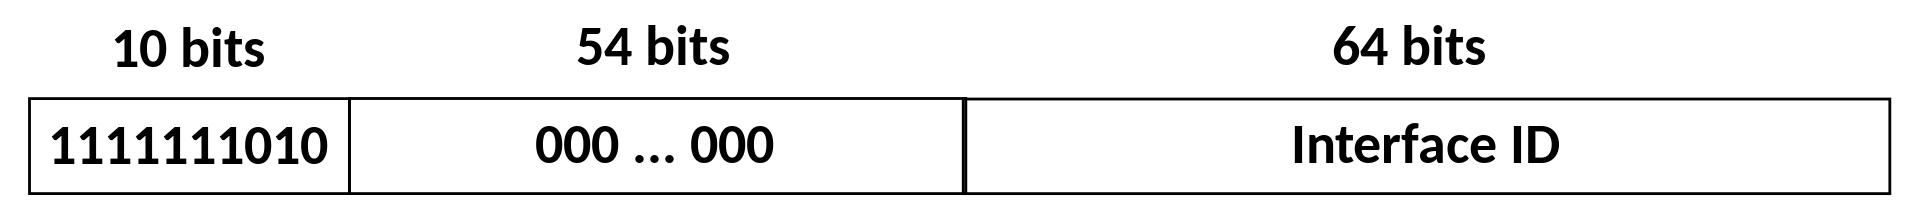
\includegraphics[width=10cm]{./IPv6_link_local_unicast_address_structure-en.svg.PNG}
%\vspace{-10pt}
\caption{IPv6 8-bytes Format }\label{fig:ipv6-8bytes}
\end{wrapfigure}


In the Internet Protocol Version 6 (IPv6), the address block fe80::/10 has been reserved for link-local unicast addressing.\footnote{\label{linklokal} R. Hinden; \href{https://en.wikipedia.org/wiki/Steve_Deering}{S. Deering} (February 2006). \href{https://datatracker.ietf.org/doc/html/rfc4291}{IP Version 6 Addressing Architecture}. IETF. doi:10.17487/RFC4291. RFC 4291. Updated by RFC 5952, RFC 6052, RFC 7136, RFC 7346, RFC 7371, RFC 8064.}}${}^{{}^{2 \cdot 4}}$ (IETF), RFC 2} Of the 64 bits of a link-local addresses' network component, the most significant 10 bits (1111111010) (Fig. \ref{fig:ipv6-8bytes}) correspond to the IANA-reserved "global routing prefix" for link-local addresses, while the "subnet ID" (the remaining 54 bits) is zero$.^{\footnotemark[6 \ref{linklokal}^{2\cdot 5 \cdot}]}$ 

Unlike IPv4, IPv6 requires a link-local address on every network interface on which the IPv6 protocol is enabled, even when routable addresses are also assigned$.^{\footnotemark[8 \ref{linklokal}^{2\cdot}]}$ 

Consequently, IPv6 hosts usually have more than one IPv6 address assigned to each of their IPv6-enabled network interfaces. The link-local address is required for IPv6 sublayer operations of the Neighbor Discovery Protocol, as well as for some other IPv6-based protocols, such as DHCPv6.

When using an IPv6 link-local address to connect to a host, a zone index must be added to the address so that the packets can be sent out on the correct interface.

In IPv6, addresses may be assigned by stateless (automatic) or stateful (manual) mechanisms. Stateless address autoconfiguration is performed as a component of the Neighbor Discovery Protocol (NDP).\footnote{\label{NDP} S. Thomson; T. Narten; T. Jinmei (September 2007). \href{https://datatracker.ietf.org/doc/html/rfc4862}{IPv6 Stateless Address Autoconfiguration}. Network Working Group. doi:10.17487/RFC4862. RFC 4862. Obsoletes RFC 2462. Updated by RFC 7527.} The address is formed from its routing prefix and a unique identifier for the network interface.

Through NDP routing prefix advertisements, a router or server host may announce configuration information to all link-attached interfaces which causes additional IP address assignment on the receiving interfaces for local or global routing purposes. This process is sometimes also considered stateless, as the prefix server does not receive or log any individual assignments to hosts. Uniqueness is guaranteed automatically by the address selection methodology. It may be MAC-address based$,^{\footnotemark[1 \ref{NDP}]}$  or randomized.\footnote{\label{randomized} F. Gont; S. Krishnan; T. Narten; R. Draves (February 2021). \href{https://datatracker.ietf.org/doc/html/rfc8981}{Temporary Address Extensions for Stateless Address Autoconfiguration in IPv6}. IETF. doi:10.17487/RFC8981. ISSN 2070-1721. RFC 8981. Obsoletes RFC 4941.} Automatic duplicate address detection algorithms prevent assignment errors.



\section{IPv4}

Internet Protocol version 4 (IPv4) is the fourth version of the Internet Protocol (IP). It is one of the core protocols of standards-based internetworking methods in the Internet and other packet-switched networks.

\begin{wrapfigure}{3cm}
\centering
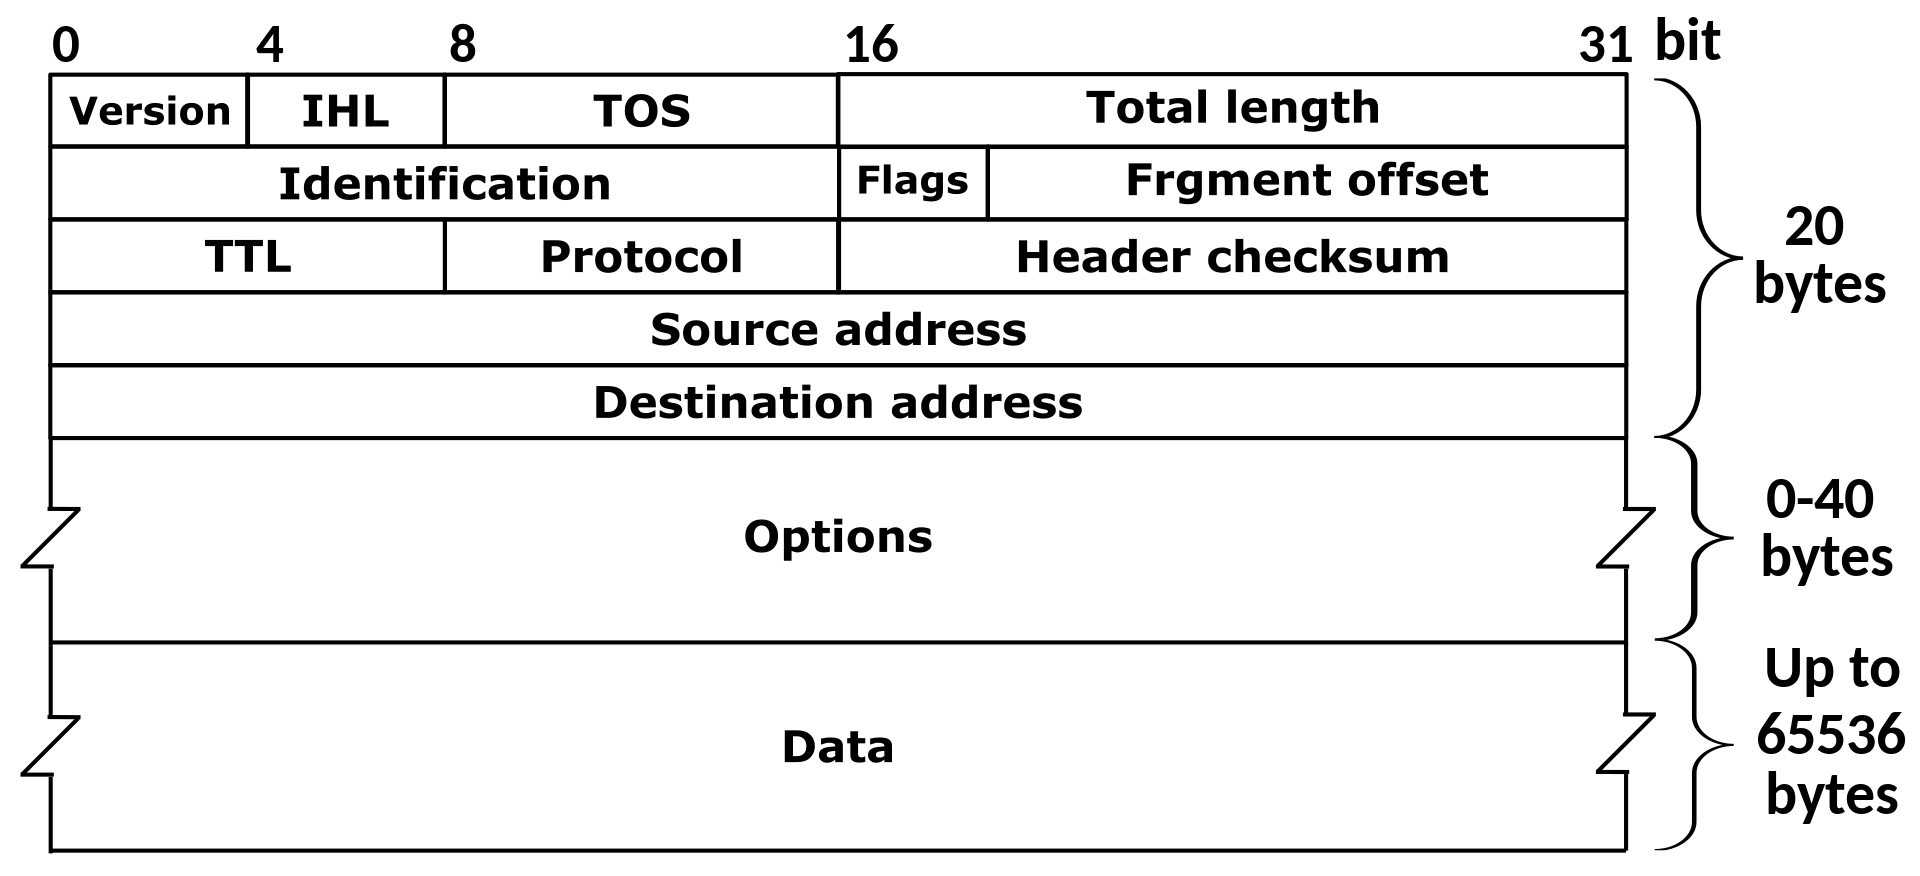
\includegraphics[width=10cm]{./IPv4_Packet-en.svg.PNG}
%\vspace{-10pt}
\caption{IPv6 8-bytes Format }\label{wrap-fig:9}
\end{wrapfigure}

IPv4 was the first version deployed for production on SATNET in 1982 and on the ARPANET in January 1983. It is still used to route most Internet traffic today,\footnote{\label{note2}\href{http://bgp.potaroo.net/index-bgp.html}{"BGP Analysis Reports"}. Retrieved 2013-01-09.} even with the ongoing deployment of Internet Protocol version 6 (IPv6),\footnote{\label{note3}\href{https://www.google.com/intl/en/ipv6/statistics.html}{"IPv6 – Google"}. www.google.com. Retrieved 2022-01-28.} its successor.

IPv4 uses a 32-bit address space which provides 4,294,967,296 ($2^{32}$) unique addresses, but large blocks are reserved for special networking purposes.\footnote{\label{note4}\href{https://www.iana.org/assignments/iana-ipv4-special-registry/iana-ipv4-special-registry.xhtml}{"IANA IPv4 Special-Purpose Address Registry"}. www.iana.org. Retrieved 2022-01-28.} \footnote{\label{note5}\href{https://datatracker.ietf.org/doc/html/rfc5735}{"RFC 5735 - Special Use IPv4 Addresses"}. datatracker.ietf.org. Retrieved 2022-01-28.}




\subsection{conversion to binary}

First a couple of words on the binary code first. A binary code is essentially text, computer processor low level instructions, or any other data using a two-symbol system. The two-symbol system used is often "0" and "1" from the \textbf{binary number system}. The binary code assigns a pattern of bits (aka binary digit), to each character, instruction, etc. For example, a binary string of eight bits can represent any of 256 possible values and can, therefore, represent a wide variety of different items.
In computing and telecommunications, binary codes are used for various methods of encoding data, such as character strings, into bit strings. 

Let's now convert 192.168.2.7 into binary
\newline

\begin{tabular}{||l|c|r|p{5cm}||}
    Division by 2 & Quotient & Remainder & Notes \\
    192/2 & 96 & 0 & This will be the 8th bit \\
    96/2 & 48 & 0 & The 7th bit \\
    48/2 & 24 & 0 & The 6th bit \\
    24/2 & 12 & 0 & The 5th bit \\
    12/2 & 6 & 0 & The 4th bit \\
    6/2 & 3 & 0 & The 3th bit \\
    3/2 & 1 & 1 & The 2nd bit \\
    1/2 & 0 & 1 & The 1st bit \\
\end{tabular}

\section{binary to Hex}

The hexadecimal system uses the number 16 as its base. As a $base^{16}$ numeral system, it uses 16 symbols. These are the 10 decimal digits 

\[0, 1, 2, 3, 4, 5, 6, 7, 8, 9\] and the first six letters of the English alphabet \[A, B, C, D, E, F\] which are representing the values 10, 11, 12, 13, 14 and 15.
This is useful in mathematics and IT as a more friendly way to represent binary. Each hex digit represents four binary digits; therefore you could say hex is a language to write binary in an abbreviated form.
Four binary digits make up half a byte. This means one byte can carry binary values from 0000 0000 to 1111 1111. In hex, these can be represented ranging from 00 to FF.
In html programming, colors can be represented by a 6-digit hexadecimal number: FFFFFF represents white whereas 000000 represents black.
Hex is more friendly in terms of possibility. It goes from 0 to 9 and then from A to F. It's 
The calculator has a \textbf{programmer} mode which allows you to use hex as well

\section{IP config}
Displays all current TCP/IP network configuration values and refreshes Dynamic Host Configuration Protocol (DHCP) and Domain Name System (DNS) settings. Used without parameters, ipconfig displays Internet Protocol version 4 (IPv4) and IPv6 addresses, subnet mask, and default gateway for all adapters.

\subsection{ipconfig/all}
Displays the full TCP/IP configuration for all adapters. Adapters can represent physical interfaces, such as installed network adapters, or logical interfaces, such as dial-up connections.

\subsection{ipconfig/displaydns}
Displays the contents of the DNS client resolver cache, which includes both entries preloaded from the local Hosts file and any recently obtained resource records for name queries resolved by the computer. The DNS Client service uses this information to resolve frequently queried names quickly, before querying its configured DNS servers.

The fields in the output of /displaydns correspond to the fields of an actual DNS reply.

\begin{itemize}
\item{In a DNS server's database, each piece of data is a "resource record".}
\item{"Record name" is the name you query DNS for, and the records (addresses or something else) belong to that name.}
\item{"Record type" is the type, displayed as a number - although more commonly they are referred to by their names, internally (in the DNS protocol) each has a number. Type 1 is "A" for "address", an IPv4 address. (IPv6 uses type 28, "AAAA", for an address four times as long.) "PTR", type 12, is a "pointer" to a hostname - most commonly used when mapping an IP address back to its name. "CNAME" is "canonical name".}
\item{"Time To Live" is the time in seconds after which the cache entry must expire.}
\item{"Data Length" appears to be the length in bytes - an IPv4 address is four bytes, IPv6 is sixteen bytes. For CNAME or PTR, Windows displays a static number (either 4 or 8, depending on your system) - this is actually the size of a memory address where the actual text is kept.}
\item{The "answer" section of a DNS reply is the actual answer to the query, and "additional" contains information that will likely be needed to find the actual answer. For example, glue records.}
\item{"<type> record" shows the actual value stored.}
\end{itemize}


%\subsection{ipconfig/flushdns}
%Flushes and resets the contents of the DNS client resolver cache. During DNS troubleshooting, you can use this procedure to discard negative cache entries from the cache, as well as any other entries that have been added dynamically.

\subsection{ipconfig/registerdns}
Initiates manual dynamic registration for the DNS names and IP addresses that are configured at a computer. You can use this parameter to troubleshoot a failed DNS name registration or resolve a dynamic update problem between a client and the DNS server without rebooting the client computer. The DNS settings in the advanced properties of the TCP/IP protocol determine which names are registered in DNS.

\subsection{ipconfig/flushdns}

By default, most operating systems will cache IP addresses and other Domain Name System (DNS) records in order to fulfill future requests more quickly.

For example, when I type in https://lonezscents.com/ in my browser’s address bar for the first time, the browser has to ask DNS servers where to find the site. Once it has that information, the browser can store it in its local cache. Then, the next time I type in that website address, the browser will look for its DNS information in the local cache first and be able to find the site more quickly.

The problem is that sometimes dangerous IP addresses or corrupted results can be cached and need to be removed. The DNS cache can also impact your ability to connect to the internet or cause other issues. Whatever the reason, all major operating systems allow you to force the process of clearing this cache — or “flushing DNS.”

\subsubsection{what flush DNS does}
Flushing DNS will clear any IP addresses or other DNS records from your cache. This can help resolve security, internet connectivity, and other issues.

It’s important to understand that your DNS cache will clear itself out from time to time without your intervention. That’s because the DNS cache — in addition to saving all information that’s relevant to identifying and finding a website — also saves a component called TTL, or time to live. This specifies a period of time (in seconds) in which the DNS record for a site remains valid. Within this time period, any queries to the website are answered from the local cache without the help of the DNS server. Once the TTL expires, the entry will be removed from the cache.

However, there are reasons you may need to force a DNS flush rather than wait for the TTL of all the entries to expire. Let’s take a look at why below.

\subsubsection{why would you flush DNS}

There’s a few reasons you might need to flush your DNS cache. These reasons may have to do with security, technical problems, or data privacy. Let’s briefly cover each one below.

\begin{itemize}
\item{\textbf{You want to prevent DNS spoofing}.
DNS spoofing — also known as DNS cache poisoning — is an attack in which bad actors gain access to your DNS cache and alter the information in order to redirect you to the wrong sites. In some cases, they will redirect you to a fraudulent website that resembles its intended destination so that you enter in sensitive information, like your online banking login information.}

\item{\textbf{You’re seeing a 404 error}.
Let’s say you’ve cached the DNS information of a site that’s since moved to a new domain name or host. In that case, the DNS information on your computer may not get updated right away and you could end up seeing a 404 error or an outdated version of a site when you try to visit. Although the information will eventually get updated in your DNS cache, you don’t have to wait. You can clear DNS cache at any time.}

\item{\textbf{You’re having trouble accessing a website}.
If you’re having trouble getting a website to load, then you should try other steps first, like clearing your browser's temporary files and cookies and adjusting your browser settings to turn off pop-up blockers and allow sites to save and read cookies. But if you’ve exhausted your options, then you can flush DNS to reset your computer's connection to the internet.}

\item{\textbf{You want to keep your search behavior private}.
When you think of tracking user behavior on the internet, you probably think of cookies — but the DNS cache can reveal your search history as well. That’s because the DNS cache is designed to act like a virtual address book, storing the information of the websites you visit regularly. To keep this information away from data collectors or bad actors on the web, it’s a good idea to regularly flush your DNS cache.}
\end{itemize}
Now that we understand what flushing your DNS cache means and why you’d want to, let’s walk through how you can do it below.



\section{DHCP}

DHCP (Dynamic Host Configuration Protocol) is a protocol that provides automatic, and centralized management for the distribution of IP addresses within a network. It's also used to configure the subnet mask, default gateway, and DNS server information on the device. It comes handy in case the BYOD trend is applied in the workplace.

\subsection{BYOD}
BYOD is the concept of employees using their personally owned device(s) for work purposes.With BYOD, an organisation has ownership of the corporate data and resources that may be accessed or stored on a device, but the device itself is the property of the user.

\medskip

This aims to:
\begin{itemize}
\item{Give end-users the ability to use IT they feel comfortable with}
\item{Reduce overheads for the organisation in terms of procurement and provisioning of corporate devices}
\item{Enable flexible (including remote) working}
\item{Increase productivity}
\item{Provide redundancy to business and organisations when workers are unable to access their main places of work}
\end{itemize}

\subsection{ipconfig /release}

If you give this command in the prompt then you'll get prompted with an IP address line showing 0.0.0.0 as the IP address. This is normal because the command releases the IP address from the network adapter. During this time, your computer has no IP address and cannot access the internet.

\subsection{ipconfig/ renew}
The host asks the router to drop the network configuration and make a new one. When the command is finished, a new line appears at the bottom of the Command Prompt screen that contains an IP address.


Bring your own device

\subsection{vulnerabilities in LAN}
Poor configuration and Poor encryption

\subsubsection{Poor configuration}

\subsubsection{Poor encryption}


\subsection{Fixed IP}
So that someone doesn't just plug a device and gets an IP-address from DHCP. A device needs to be approved in order to receive an IP

\section{dns root server}
There are 13 important DNS root servers on the internet that store a complete database of domain names and their associated public IP addresses. These top-tier DNS servers are named A through M for the first 13 letters of the alphabet.Ten of these servers are in the US, one in London, one in Stockholm, and one in Japan 

\paragraph{why 13 DNS servers?}
\begin{flushleft}
That's exactly how much we need with IPv4. The IP packet size is 2 bytes.
\end{flushleft}

\subsection{who manages}
The Internet Assigned Numbers Authority (IANA) keeps this list of DNS root servers if you're interested. ICANN manages them as well by delegating to IANA. It stands for Internet Corporation for Assigned Names and Numbers.

\section{The DNS Service}
The DNS service is what a server running DNS software offers. Today, the DNS service is a very popular offer. The DNS service can be run on a separate server, which is effective if running a very large and popular website, and can also be run on a \textbf{shared hosting server}\footnote{\label{sharedHostingServer}A type of service where one physical server is hosting multiple websites. The server’s resources are allocated to its many users, so there is a low cost for using this type of hosting}, which is sufficient in 90\% of the cases.

Here follows a main differentiation between servers:
\begin{itemize}
\item{recursive = non-authoritative}
\item{non-recursive = authoritative}
\end{itemize}


\section{The four DNS Servers to load a webpage}
Once a DNS query is entered, it passes through a few different servers before resolution, without any end-user interaction.

\subsection{DNS recursor}

This is a server designed specifically to receive queries from client machines. It tracks down the DNS record and makes additional requests to meet the DNS queries from the client. The number of requests can be decreased with DNS caching when the requested resources are returned to the recursor early on in the lookup process.

\subsection{Root name server}

This server does the job of translating the human-friendly hostnames into computer-friendly IP addresses. The root server accepts the recursor’s query and sends it to the TLD nameservers in the next stage, depending on the domain name seen in the query.

\subsection{DNS server}

Top-Level Domain (TLD) nameserver DNS servers are usually public. But you can have a \textbf{private DNS} too if you want to keep information private or prefer a particular way to perform server management/administration.

The TLD nameservers are responsible for maintaining the information about the domain names. For example, they could contain information about websites ending in “.com” or “.org” or country-level domains like “www.example.com.uk”, “www.example.com.us”, and others. The TLD nameserver will take the query from the root server and point it to the authoritative DNS nameserver associated with the query’s particular domain.




\subsection{Authoritative nameserver}

In the last step, the authoritative DNS nameserver will return the IP address back to the DNS recursor that can relay it to the client. This authoritative DNS nameserver is the one at the bottom of the lookup process that holds the DNS records. Think of these as the last stop or the final authoritative source of truth in the process.

The DNS Security Extensions (\textbf{DNSSEC}) is a set of specifications that extend the DNS protocol by adding cryptographic \textbf{dns authentication} for responses received from authoritative DNS servers. Its goal is to defend against techniques that hackers use to direct you somewhere else. You can safely assume you really got the answer from that DNS server and not by someone trying to act like a DNS server. 

\section{PING}
Ping is a tool to test the reachability of a host on an IP network. It measures the round-trip time for messages sent from the originating host to a destination computer that are echoed back to the source.

Ping operates by means of Internet Control Message Protocol (\textbf{ICMP}) packets. Pinging involves sending an ICMP echo request to the target host and waiting for an ICMP echo reply. The program reports errors, packet loss, and a statistical summary of the results like round-trip time.

\section{Loopback}
Loopback (also written loop-back) is the routing of signals back to their source to test the communications infrastructure. The address is 127.0.0.1. We were planning to use it for our app on Android before the server went actually online

\section{Subnet}
A subnetwork or subnet is a logical subdivision of an IP network. The practice of dividing a network into two or more networks is called subnetting.

Computers that belong to the same subnet are addressed with an identical most-significant bit-group in their IP addresses. This results in the logical division of an IP address into two fields: the network number or routing prefix and the rest field or host identifier. The rest field is an identifier for a specific host or network interface.

\subsection{Routing prefix expressed in CIDR}
All we need to do to write it in this notation is to write address of a network, followed by a slash character (/), and ending with the bit-length of the prefix. For example, 198.51.100.0/24 is the prefix of the Internet Protocol version 4 network starting at the given address, having 24 bits allocated for the network prefix, and the remaining 8 bits reserved for host addressing. Addresses in the range 198.51.100.0 to 198.51.100.255 belong to this network, with 198.51.100.255 as the subnet broadcast address. The IPv6 address specification 2001:db8::/32 is a large address block with 296 addresses, having a 32-bit routing prefix.For example, 198.51.100.0/24 is the prefix of the network starting at the given address, having 24 bits allocated for the network prefix, and the remaining 8 bits reserved for host addressing. Addresses in the range 198.51.100.0 to 198.51.100.255 belong to this network, with 198.51.100.255 as the subnet broadcast address.The prefix 198.51.100.0/24 would have the subnet mask 255.255.255.0.A router serves as a logical or physical boundary between the subnets.


\subsubsection{the different CIDR classes}
\begin{itemize}
\item{Class A: 255.0.0.0 (16.777.216 addresses)​}
\item{Class B: 255.255.0.0 (65.536 addresses)​}
\item{Class C: 255.255.255.0 (256 addresses)​}
\end{itemize}

\section{Broadcast address}
A broadcast address is a network address used to transmit to all devices connected to a multiple-access communications network. A message sent to a broadcast address may be received by all network-attached hosts.In contrast, a multicast address is used to address a specific group of devices, and a unicast address is used to address a single device. 

\begin{itemize}
\item{At \textbf{network layer}, a broadcast address may be a specific IP address.}
\item{At \textbf{data link layer} on Ethernet networks, it is a specific MAC address}
\end{itemize}

\subsection{single Broadcast address}
This is a condition which is consequence of having only one subnet, creating unnecessary traffic if the network is too big and people are getting packets they're not interested to. One solution is to subnet the network creating a subnet that only contains the subscribers to the broadcast and leave all the others in peace

%A task left is to create 2 subnets in the same local network

\subsection{VLAN}
This is to make sure every subnet is isolated.A VLAN is a logical subnetwork that groups a collection of devices from different physical LANs. It's used to re-partition a network for improved traffic management



\section{Multicast}
In computer networking, multicast is group communication where data transmission is addressed to a group of destination computers simultaneously. Multicast can be one-to-many or many-to-many.

Group communication may either be application layer multicast or network-assisted multicast where the application layer sends the packet to the multicast address and then copies are automatically created in other network elements, such as routers, switches etc, to all network segments that currently contain members of the group. 
Multicast is often employed in streaming media or videoconferencing.

The Internet Group Management Protocol (\textbf{IGMP}) is the protocol that allows devices to share one IP address, allowing them to join a multicasting group so they can all receive the same data. 



\section{Unicast}
In computer networking, unicast is a one-to-one transmission from one point in the network to another point; that is, one sender and one receiver, each identified by a network address.\footnote{\label{unicast}Godred Fairhurst \href{https://www.erg.abdn.ac.uk/users/gorry/course/intro-pages/uni-b-mcast.html}{"Unicast, Broadcast, and Multicast"}.}

Unicast is in contrast to multicast and broadcast which are one-to-many transmissions.

Internet Protocol unicast delivery methods such as Transmission Control Protocol (TCP) and User Datagram Protocol (UDP) are typically used.

\section{The Five IPv4 Classes}
In the IPv4 IP address space, there are five classes: A, B, C, D and E. Each class has a specific range of IP addresses (and determines the number of devices you can have per network). Primarily, class A, B, and C are used by the majority of devices on the Internet. Class D and class E are for special uses.

\medskip
\noindent Here we go with the list:

\subsection{Class A Public & Private IP Address Range}
Class A addresses are for networks with large number of total hosts. Class A allows for 126 networks by using the first octet for the network ID. \textbf{The first bit in this octet, is always zero}. The remaining seven bits in this octet complete the network ID. The 24 bits in the remaining three octets represent the hosts ID and allows for approximately 17 million hosts per network. Class A network number values begin at 1 and end at 127.

\begin{itemize}
\item{Public IP Range: 1.0.0.0 to 127.0.0.0}
\item{First octet value range from 1 to 127}
\item{Private IP Range: 10.0.0.0 to 10.255.255.255}
\item{Subnet Mask: 255.0.0.0 (8 bits)}
\item{Number of Networks: 126}
\item{Number of Hosts per Network: 16,777,214}
\end{itemize}
 \clearpage
\subsection{Class B Public & Private IP Address Range}
Class B addresses are for medium to large sized networks. Class B allows for 16,384 networks by using the first two octets for the network ID. Here the \textbf{mnemonic} is that \emph{The first two bits in the first octet are always \textbf{1 0}}. The remaining six bits, together with the second octet, complete the network ID. The 16 bits in the third and fourth octet represent host ID and allows for approximately 65,000 hosts per network. Class B network number values begin at 128 and end at 191.

\begin{itemize}
\item{Public IP Range: 128.0.0.0 to 191.255.0.0}
\item{First octet value range from 128 to 191}
\item{Private IP Range: 172.16.0.0 to 172.31.255.255}
\item{Subnet Mask: 255.255.0.0 (16 bits)}
\item{Number of Networks: 16,382}
\item{Number of Hosts per Network: 65,534}
\end{itemize}

\subsection{Class C Public & Private IP Address Range}
Class C addresses are used in small local area networks (LANs). Class C allows for approximately 2 million networks by using the first three octets for the network ID. \textbf{A good mnemonic} for a class C IP address is that, \emph{the first three bits of the first octet are always \textbf{1 1 0}}. And the remaining 21 bits of first three octets complete the network ID. The last octet (8 bits) represent the host ID and allows for 254 hosts per network. Class C network number values begins at 192 and end at 223.

\begin{itemize}
\item{Public IP Range: 192.0.0.0 to 223.255.255.0}
\item{First octet value range from 192 to 223}
\item{Private IP Range: 192.168.0.0 to 192.168.255.255}
\item{Special IP Range: 127.0.0.1 to 127.255.255.255}
\item{Subnet Mask: 255.255.255.0 (24 bits)}
\item{Number of Networks: 2,097,150}
\item{Number of Hosts per Network: 254}
\end{itemize}
\clearpage
\subsection{Class D IP Address Range}
Class D IP addresses are not allocated to hosts and are used for multicasting. Multicasting allows a single host to send a single stream of data to thousands of hosts across the Internet at the same time. It is often used for audio and video streaming, such as IP-based cable TV networks. Another example is the delivery of real-time stock market data from one source to many brokerage companies.

\begin{itemize}
\item{Range: 224.0.0.0 to 239.255.255.255}
\item{First octet value range from 224 to 239}
\item{Number of Networks: N/A}
\item{Number of Hosts per Network: Multicasting}
\end{itemize}


\subsection{Class E IP Address Class}
Class E IP addresses are the weird ones. They're not allocated to hosts and are not available for general use. These are reserved for research purposes.

\begin{itemize}
\item{Range: 240.0.0.0 to 255.255.255.255}
\item{First octet value range from 240 to 255}
\item{Number of Networks: N/A}
\item{Number of Hosts per Network: Research/Reserved/Experimental}
\end{itemize}

\begin{wrapfigure}[10]{R}{6cm}
\centering
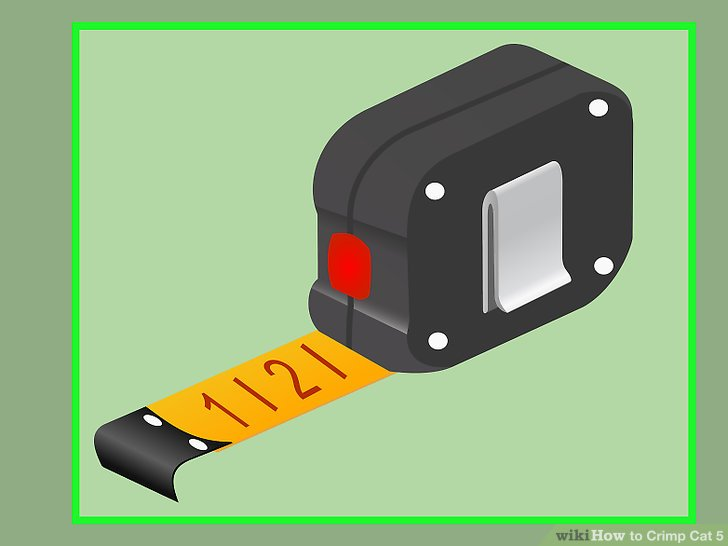
\includegraphics[width= 6cm]{./meter.JPG}
%\vspace{-10pt}
\caption{tools to measure the cable}\label{fig:meter}
\end{wrapfigure}

\section{How to Crimp Cat 5}
Category-5 cable (or Cat-5 cable) is probably one of the most common cable tipe used in networking.
If you're thinking to build a large network, maybe cutting and crimping by yourself can make you save money. The followings are the steps needed to cut and crimp your own. If it's a small network you can buy pre-made ones rather than buy the tools and bulk spools of cable. But to be fair if you ain't go problems with your hands, in the long run, it'll be better to crimp your own. Takes time and patience though. After doing one cable with the help of Beth I felt like making cables from scratch should be paid 20£ an hour at least

\subsection{Decide how much Cat-5 cable you need}
If you only need just the cable to wire a home network or other small network, as I said, consider buying cables in finished lengths from a computer supply store. If your needs are larger, come up with a rough estimate of the total length of cable you need. See fig \ref{fig:meter} for an example of tool to take measures with

\clearpage

\begin{wrapfigure}[10]{R}{6cm}
\centering
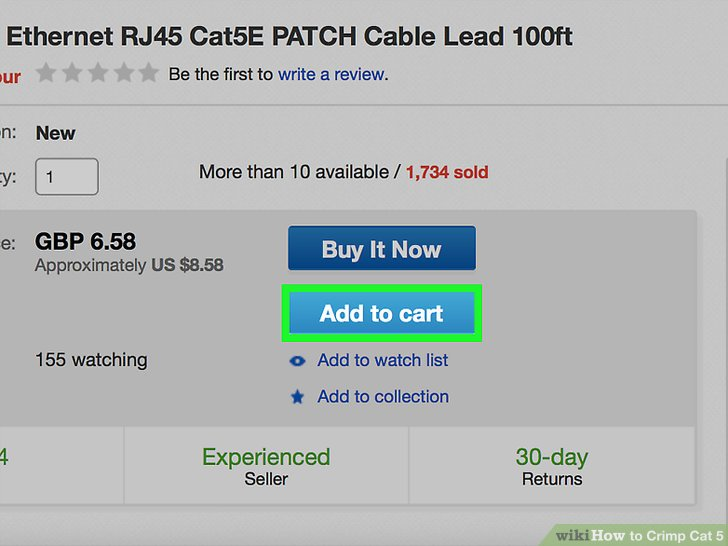
\includegraphics[width= 6cm]{./step2.JPG}
%\vspace{-10pt}
\caption{step 2}\label{fig:step2}
\end{wrapfigure}

\subsection{Purchase the items you will need to build the cables}
You will need to buy 3 things: a length of Cat-5 cable, as many RJ-45 heads as you need, and a wire crimping tool. Cat-5 cable is best purchased from small computer supply stores; larger chain stores are less likely to carry bulk spools of cable. The plastic ends of the cables are called RJ-45 heads, and can also be purchased from computer supply stores. Each cable needs 2 heads, so buy twice as many as the number of cables you want to make. When buying a Cat-5 crimping tool, look for a model that includes a wire snipping tool. To be conservative, buy more cable and heads than you think you need. look fig \ref{fig:step2}

\begin{wrapfigure}[10]{R}{6cm}
\centering
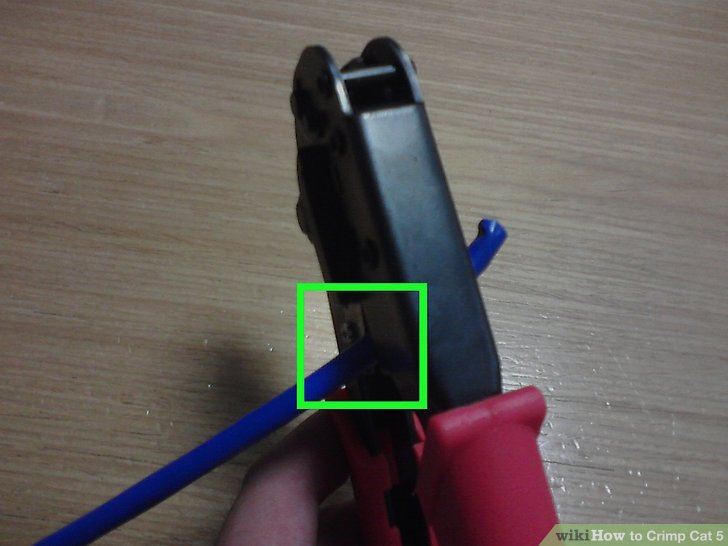
\includegraphics[width= 6cm]{./step3.JPG}
%\vspace{-10pt}
\caption{step 3}\label{fig:step3}
\end{wrapfigure}

\subsection{Cut the cable to lenght}
Determine the length needed for your cable and use the wire cutting tool on the crimping tool to cut the cable to this length. See pic \ref{fig:step3}

\begin{wrapfigure}[10]{L}{6cm}
\centering
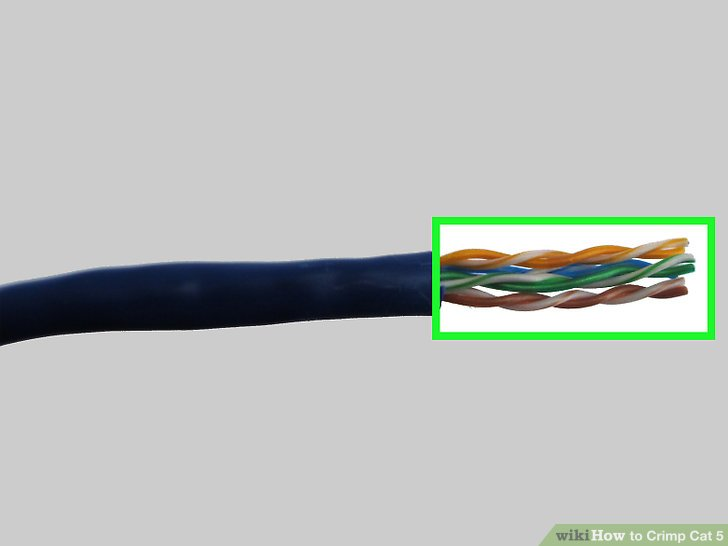
\includegraphics[width= 13cm]{./step4.JPG}
%\vspace{-10pt}
\caption{step 4}\label{fig:step4}
\end{wrapfigure}

\subsection{Prepare the ends of the cable for crimping}
Use the wire cutting tool to strip away about half an inch of the outer coating on each end of the cable. You will see 8 small colored wires twisted into 4 pairs. Carefully untwist each pair so that each of the 8 wires is separate. Now arrange the wires in the proper order. From left to right, put the wires in this order: green and white, green, orange and white, blue, blue and white, orange, brown and white, brown. See pic \ref{fig:step4}
\clearpage 

\begin{wrapfigure}[11]{R}{12cm}
\centering
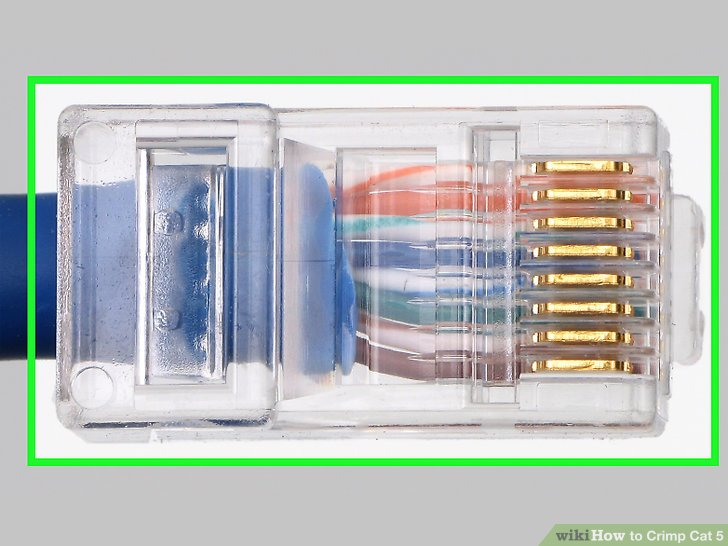
\includegraphics[width= 10cm]{./step5.JPG}
%\vspace{-10pt}
\caption{step 5}\label{fig:step5}
\end{wrapfigure}

\subsection{Place the Cat-5 cable ends into the RJ-45 heads}
See pic \ref{fig:step5}

\subsection{Determine the orientation of the wires}
See pic.

\subsection{Line the 8 wires up neatly so that they will fit into the plastic head}
Carefully insert the wires (all at once) into the plastic head, pushing them in as far as they will go. The exposed wires should line up with the 8 small metal contacts in the head.

\subsection{Crimp the head onto the cable}
Place the plastic head into the appropriate slot in the crimping tool, being careful not to misplace the 8 wires. With the head positioned properly, apply pressure to the crimper's handles to clamp the head down onto the wires. The metal contacts should now be touching each of the 8 wires. Repeat this process on the other end of the cable.

\subsection{Test your cable if desired}
Test your cable if desired. If you have a cable testing tool, insert both ends of your finished cable into the tool to check for a signal. The cable should now be ready to use.

\section{Choose the Antivirus}
The followings are the criteria that you should use to select the best security product:

\subsection{Look for all-inclusive protection}
Long time ago, having a good security product for your computer meant that it was enough to have an antivirus. Today you also need to worry about firewall, cybercrime on websites, ransomware (never happened to me. I guess because I've been always able to tell if something is dodgy), VPN protection against monitoring and censorship, etc.
A good security product today must protect you against the following types of threats:

\begin{itemize}
\item{\textbf{Viruses} - programs with malicious intents which can infect other devices via an executable file but to get infected for real you have to run it.}
\item{\textbf{Trojans (Horses)} - are malicious software that can look like normal software and because of that, you download and run them. When you do that, trojans usually open some port numbers creating a gate to other unwanted stuff.}
\item{\textbf{Worms} - are malicious programs that take advantage of the security holes and vulnerabilities in your operating system or other software like your web browser, that's why is good to have everything updated. If you get a worm that's it, you have it. No need to run it. You're infected already. It's not like a virus that needs to be run}
\item{\textbf{Spyware} - software programs that are designed to spy and gather info about you and send them back to criminals.}
\item{\textbf{Rootkits} - a malware designed to give hackers remote access and control of a device, targeting a vulnerability in the operating system so the hacker gains remote access with root privileges.}
\item{\textbf{Ransomware} - malicious programs that, once they infect your computer, they take control and encrypt your files, like your pictures, work documents, and videos. Once that happens, ransomware programs try to make you pay some money to their creators, so that you can get your files back. I wouldn't pay a bloody pence. Who's going to guarantee that I get my files back? And even if I do they could be infected with other rubbish. The first thing I'd do is go to my bank branch and talk to them. Once my money is safe I'll ignore the attacker as nothing ever happened. Change all the passwords. Open another bank account worst case scenario. Go to the employer and talk to them}
\item{\textbf{Adware} - software programs that display annoying advertisements on your screen, in your web browsers or other places on your computer. It may not be malware by definition, but adware almost always hurts your computer's performance and your user experience, and can also help infect your computer with malware. I had it more than once and usually I had to delete the folder where the browser is saving temp files and then uninstall and reinstall the browser. Takes a couple of attempts. As a last resort formatting the device}
\item{\textbf{Network attacks} - when hackers try to take control of your devices remotely. That is when you need a good firewall.}
\item{\textbf{Web threats} - your web browser should be the first in the line of defense against malware, that's the problem. That is why a good security solution has to include a web protection module that can stop you from visiting websites with malicious content. It is better to deal with malware in your browser than to have to do that when it reaches your computer. It's enough to visualize a web-page to get an Adware. Your browser shouldn't allow you to see the web-page at all. That's the problem. Even if you didn't click the dodgy link telling you you won the last i-Phone you might already got a malware. It's usually and Adware in my experience}
\end{itemize}

\clearpage

\section{VoIP}
Voice over Internet Protocol (VoIP), is a method and group of technologies for the delivery of voice/video communications over the Internet rather than via the public switched telephone network (PSTN)

\subsection{Overview}
The steps and principles involved in originating VoIP telephone calls are similar to traditional digital telephony and involve signaling, channel setup, digitization of the analog voice signals, and encoding. Instead of being transmitted over a circuit-switched network, the digital information is packetized and transmission occurs as IP packets over a packet-switched network. They transport media streams using special media delivery protocols that encode audio and video with audio codecs and video codecs. Various codecs exist that optimize the media stream based on application requirements and network bandwidth; some implementations rely on narrowband and compressed speech, while others support high-fidelity stereo codecs.

%The most widely used speech coding standards in VoIP are based on the linear predictive coding (LPC) and modified discrete cosine transform (MDCT) compression methods. Popular codecs include the MDCT-based AAC-LD (used in FaceTime), the LPC/MDCT-based Opus (used in WhatsApp), the LPC-based SILK (used in Skype), μ-law and A-law versions of G.711, G.722, and an open source voice codec known as iLBC, a codec that uses only 8 kbit/s each way called G.729.

%Early providers of voice-over-IP services used business models and offered technical solutions that mirrored the architecture of the legacy telephone network. Second-generation providers, such as Skype, built closed networks for private user bases, offering the benefit of free calls and convenience while potentially charging for access to other communication networks, such as the PSTN. This limited the freedom of users to mix-and-match third-party hardware and software. Third-generation providers, such as Google Talk, adopted the concept of federated VoIP.[1] These solutions typically allow dynamic interconnection between users in any two domains of the Internet, when a user wishes to place a call.

%In addition to VoIP phones, VoIP is also available on many personal computers and other Internet access devices. Calls and SMS text messages may be sent via Wi-Fi or the carrier's mobile data network.[2] VoIP provides a framework for consolidation of all modern communications technologies using a single unified communications system.

%pulses - digital
VoIP phones use \textbf{digital tones} rather than \textbf{pulses} which phased out long time ago. Pulse dialing uses a number of signal pulses to indicate the phone number that was entered whereas tone dialing uses specific tones to indicate the number. It takes a longer time to dial a number on a rotary phone with pulse dialing than it takes on a tone dialing phone with a numeric keypad.


\section{Common Port Numbers and Protocols}

\subsection{Protocols}
Voice over IP has been implemented with both proprietary and open protocols.A variety of functions are needed to implement VoIP communication. Some protocols perform multiple functions, while others perform only a few. These functions include:

\begin{itemize}
\item{Network and transport – Creating reliable transmission involving acknowledging receipt of data and retransmitting data that wasn't received.}
\item{Session management – Creating and managing a session (a "call"), which is a connection between two or more peers that provides a context for further communication.}
\item{Signaling – Performing registration (advertising one's presence and contact information) and discovery (locating someone and obtaining their contact information), and call control (such as hold, mute, transfer/forwarding, dialing DTMF keys during a call to interact with an automated attendant}
\item{Media description – Determining what type of media to send (audio, video, etc.), how to encode/decode it, and how to send/receive it (IP addresses, ports, etc.).}
\item{Media – Transferring the actual media in the call, such as audio, video, text messages, files, etc.}
\item{Quality of service – Providing feedback about the media such as synchronization, statistics, etc.}
\item{Security – Implementing access control, verifying the identity of other participants (computers or people), and encrypting data to protect the privacy and integrity of the media contents and/or the control messages.}
\end{itemize}

\subsubsection{what VoIP protocols include}
\begin{itemize}
\item{Session Initiation Protocol (SIP), connection management protocol developed by the \href{https://www.ietf.org/}{IETF}}
%\item{H.323, one of the first VoIP call signaling and control protocols that found widespread implementation.[5] Since the development of newer, less complex protocols such as MGCP and SIP, H.323 deployments are increasingly limited to carrying existing long-haul network traffic.}
%\item{Media Gateway Control Protocol (MGCP), connection management for media gateways}
%\item{H.248, control protocol for media gateways across a converged internetwork consisting of the traditional PSTN and modern packet networks}
\item{Real-time Transport Protocol (RTP), transport protocol for real-time audio and video data. It runs over UDP}
\item{Real-time Transport Control Protocol (RTCP), used in conjunction with RTP providing stream statistics and status information}
\item{Secure Real-time Transport Protocol (SRTP), encrypted version of RTP}
%\item{Session Description Protocol (SDP), a syntax for session initiation and announcement for multi-media communications and WebSocket transports.}
\item{Inter-Asterisk eXchange (IAX), protocol used between Asterisk instances}
%\item{Extensible Messaging and Presence Protocol (XMPP), instant messaging, presence information, and contact list maintenance}
%\item{Jingle, for peer-to-peer session control in XMPP}
\item{Skype protocol, proprietary Internet telephony protocol suite based on peer-to-peer architecture}
\end{itemize}

\subsubsection{Asterisk }%(PBX)
Asterisk is a software used to establish and control telephone calls between endpoints, such as destinations on the public switched telephone network, and devices on VoIP networks. Its name comes from the asterisk (*) key present on every phone.

Originally designed for Linux, now runs on a variety of operating systems, including FreeBSD and macOS

\subsubsection{Session Initiation Protocol}
The Session Initiation Protocol (SIP) is a signaling protocol used for initiating, maintaining, and terminating real-time sessions that include voice, video and messaging applications. SIP is used for signaling and controlling multimedia communication sessions in applications of Internet telephony.

The protocol defines the specific format of messages exchanged and the sequence of communications of the participants. SIP is a text-based protocol, incorporating many elements of HTTP and SMTP protocol. A call established with SIP may consist of multiple media streams, but no separate streams are required for applications, such as text messaging, that exchange data as payload in the SIP message.SIP is designed to be independent of the underlying transport layer protocol and can be used with the User Datagram Protocol (UDP), the Transmission Control Protocol (TCP), and the Stream Control Transmission Protocol (SCTP).
 
%SIP works in conjunction with several other protocols that specify and carry the session media. Most commonly, media type and parameter negotiation and media setup are performed with the Session Description Protocol (SDP), which is carried as payload in SIP messages. For secure transmissions of SIP messages over insecure network links, the protocol may be encrypted with Transport Layer Security (TLS). For the transmission of media streams (voice, video) the SDP payload carried in SIP messages typically employs the Real-time Transport Protocol (RTP) or the Secure Real-time Transport Protocol (SRTP).

\subsubsection{Quality of service}
VoIP feels less reliable than  public telephone network because it does not provide a mechanism to ensure that data packets are not lost, and are delivered in sequential order. It is a best-effort network without fundamental quality of service (QoS) guarantees. Voice, and all other data, travels in packets over IP networks with fixed maximum capacity. This system may be more prone to data loss in the presence of congestion than traditional landlines. If there's insufficient capacity then a landline will refuse new connections while carrying the remainder without impairment, while the quality of VoIP degrades dramatically facing problems with latency, packet loss, and jitter.

Network routers handle traffic on a first-come, first-served basis. Latency can be minimized by marking voice packets as being delay-sensitive.

Network routers on high volume traffic links may introduce latency that exceeds permissible thresholds for VoIP leading to congestion and packet loss. Here the router will ask the senders to reduce their transmission rate to alleviate the congestion. But VoIP usually uses UDP not TCP because recovering from congestion through retransmission usually entails too much latency. So QoS mechanisms can avoid the undesirable loss of VoIP packets by immediately transmitting them ahead of any queued traffic on the same link.

%VoIP endpoints usually have to wait for the completion of transmission of previous packets before new data may be sent. Although it is possible to preempt (abort) a less important packet in mid-transmission, this is not commonly done, especially on high-speed links where transmission times are short even for maximum-sized packets. An alternative to preemption on slower links, such as dialup and digital subscriber line (DSL), is to reduce the maximum transmission time by reducing the maximum transmission unit. But since every packet must contain protocol headers, this increases relative header overhead on every link traversed.

The receiver must resequence IP packets that arrive out of order and recover gracefully when packets arrive too late or not at all. Recovering gracefully means ignore the missing packets having a little audio interruption which is not a big deal

%Packet delay variation results from changes in queuing delay along a given network path due to competition from other users for the same transmission links. VoIP receivers accommodate this variation by storing incoming packets briefly in a playout buffer, deliberately increasing latency to improve the chance that each packet will be on hand when it is time for the voice engine to play it. The added delay is thus a compromise between excessive latency and excessive dropout, i.e. momentary audio interruptions.

Jitter is the variance in latency. It's a random variable obviously and it is the sum of all the individual queuing delays of all the routers along the Internet path in question.In practice, the jitter of many Internet paths is dominated by a small number (often one) of relatively slow and congested bottleneck links. It keeps changing so it's an estimation

%A number of protocols have been defined to support the reporting of quality of service (QoS) and quality of experience (QoE) for VoIP calls. These include RTP Control Protocol (RTCP) extended reports,[20] SIP RTCP summary reports, H.460.9 Annex B (for H.323), H.248.30 and MGCP extensions.

%The RTCP extended report VoIP metrics block specified by RFC 3611 is generated by an IP phone or gateway during a live call and contains information on packet loss rate, packet discard rate (because of jitter), packet loss/discard burst metrics (burst length/density, gap length/density), network delay, end system delay, signal/noise/echo level, mean opinion scores (MOS) and R factors and configuration information related to the jitter buffer. VoIP metrics reports are exchanged between IP endpoints on an occasional basis during a call, and an end of call message sent via SIP RTCP summary report or one of the other signaling protocol extensions. VoIP metrics reports are intended to support real-time feedback related to QoS problems, the exchange of information between the endpoints for improved call quality calculation and a variety of other applications.

\subsection{use VoIP with satellite internet}
You can use most VoIP plans with satellite internet, but it will eat up your internet data. 

%Most satellite internet customers in the US can get VoIP service with their Viasat or HughesNet plan, which is what we recommend.
\noindent Popular internet phone providers like Skype use a lot of internet data with each call.  A Skype phone call can use up to 4 GB an hour. For satellite internet customers with low data caps, this can lead to huge fees. Using Skype for just two hours per week could use up 32 GB of data in a month.

\subsubsection{Benefits of using VoIP over satellite broadband}
\begin{itemize}
\item{Saves money when compared to mobile or landline phone}
\item{Delivers good service in areas without mobile coverage}
%\item{Offers unlimited local and long-distance service}
%\item{Connects remote workers to offices, call centers, and other workplaces seamlessly}
\end{itemize}

\subsubsection{CONs of VoIP}
\begin{itemize}
\item{you can't geo-localize an emergency VoIP phonecall}
\end{itemize}

\section{Port Numbers}

\begin{tabular}{||l|c|{5cm}||}
    protocol & port \\
    DHCP & 67  \\
    DNS & 53 \\
    FTP & 21 \\
    HTTP & 80 \\
    HTTPS & 443\\
    IMAP & 143  \\
    POP3 & 110\\
    RDP & 3389 \\
    SMTP & 25 \\
    SSH & 22\\
    TELNET & 23\\
\end{tabular}

\chapter{Emerging Technologies}
\AddToShipoutPictureBG*{
\includegraphics[width=\paperwidth,height=\paperheight]{118.jpg}}

(AI), and automation - and the ​

potential implications for digital activities. ​

\clearpage
\section{Wireless Emerging Technologies}

\subsection{Fifth generation mobile}​

5G (which stands for fifth generation) is the next step in mobile technology, following on from 4G before it and 3G before that, and like the jump from 3G to 4G, you’ll be getting far higher speeds than on any of the technologies that came before.

\subsubsection{How does it work?}
Works like 4G but the frequencies used by 5G are higher which means shorter range than the ones used for 4G and 3G though. Meaning more repetitors are required to cover the whole UK in 5G. That's probably why someone was moaning about health related issues

\subsection{NFC}

Near Field Communication (NFC) technology allows you to make payments, exchange media, and connect devices by hovering the first device in a few inches range from the other one.This is what contactless cards are actually using.

\subsection{RFID}
Radio-frequency identification (RFID) uses electromagnetic fields to automatically identify and track tags attached to objects. An RFID system consists of a tiny radio transponder, a radio receiver and transmitter. When triggered by an electromagnetic interrogation pulse from a nearby RFID reader device, the tag transmits digital data, usually an identifying inventory number, back to the reader. This number can be used to track inventory goods. It's what is used against shoplifting

\subsection{ANT}
ANT is a technology to provides personal area networks (PANs) enabling hardware to communicate by establishing conversation protocols, rules to represent data and to send signals. It's like Bluetooth, works on low energy, but Bluetooth works one-to-one while ANT can be one-to-many. The most recent is \textbf{ANT+}, introduced in 2004 and called "the first ultra low power wireless standard".


\subsection{ZigBee}
ZigBee is like wifi but consumes less power thus improving battery life but supports less number of users.
Another difference is that ZigBee can only copy and forward a message from one device to another. 
Whether you should go with Z-wave and ZigBee or Wi-Fi depends on what’s more important to you when it comes to your smarthome experience. If you want everything to work with Google or Alexa and don’t want to add smart hub complications, then Wi-Fi devices are the best option. But if you want local, cloudless control and a smarthome you can fine-tune to the most advanced specifications then ZigBee and Z-Wave win.

\section{potential implications of AI technologies on digital activities}

\subsection{what's an AI first}
It's a set of algorithms meant to outperform humans, performing functions like thinking, judging and solving problems. These algorithms can learn meaning they could replace software developers in the future. The real need for software developer will be just to work on the AI itself.

\subsection{virtual agents}

An AI-powered virtual agent can do many things that a live agent can do. Using conversational AI, virtual agents automate the routine and repetitive call types handled by live agents today. This same experience can be scaled to chat and text as a unified application. Virtual agents are powered by a centralized cloud-based AI “brain” that connects to your customer data via APIs. With all the tools to mimic live agent behavior, virtual agents extend far beyond the capabilities of touchtone IVR, directed dialog, and simple chatbots for customer service.

\subsection{speech recognition}
It is also known as automatic speech recognition (ASR), computer speech recognition, or speech-to-text, and it is a capability which uses natural language processing (NLP) to process human speech into a written format. Many mobile devices incorporate speech recognition into their systems already.
 
%\subsection{machine learning platforms}

%\subsection{multi-factor authentication (MFA)}


\chapter{Cloud Computing}
\AddToShipoutPictureBG*{\includegraphics[width=\paperwidth,height=\paperheight]{118.jpg}}

The delivery of on demanding computing power
\clearpage

\section{Introduction}
It's meant for storage, virtual CPUs, and services like servers and computers

\section{PROs and CONs}
it's much cheaper. you don't have to move your hard drives and computers if you move. But if your connection is poor it becomes unusable. It's great for disaster recovery (ie. if your company goes on fire then what's in the cloud stays in the cloud). You don't need that expertise in your team. You can buy more storage (scalable)

\subsection{Carbon footprint}
 Some providers power their data centers with 100 percent renewable energy so, chosing wisely you could reduce consumption of CO2. 

\subsection{Scam}
Your data can be sold to other people

\section{dirty data}
Useless data like the pictures from whatsapp groups, Emails on your phone you're not reading, etc. This is what impacts on the carbon footprint

\section{Major cloud platforms}
Many companies do offer cloud platforms that support the development and management of your organisation’s IT needs.
\subsection{Azure}
Microsoft Azure is a great cloud solution for organisations that predominantly use Microsoft infrastructure and services. Azure is developed to provide flexible integration with Microsoft services such as O365 and Active Directory, enabling organisations to transform and scale existing services to a fast and reliable cloud-based solution.

\clearpage
\section{Risks using the cloud}

There are many risks using the clous. Here we list a few of them.

\subsection{Switching between providers} \flushleft
If you want to migrate, you need to find a good provider able to do it or you might experience \textbf{loss of data}. It might happen intentionally(scam) or unintentionally(human error)


\subsection{Lack of cloud expertise}

A significant risk of cloud computing is a lack of cloud expertise.To properly secure your cloud environment, you must be able to  secure and configure the architecture and integrate them with third-party services. This requires experts either employed in-house or via a third-party to ensure you can gain complete visibility of your infrastructure. You must know who has access to your cloud services and be able to maintain a security management strategy across your cloud environment.


\subsection{Cloud misconfigurations}

Gaps in your understanding of cloud security can lead to misconfigurations. Correctly configuring your cloud infrastructure is the responsibility of your organisation, not the cloud provider. One of the main causes of misconfiguration is over-privileged accounts. 

The principle of least privilege means it is important to only grant admin privileges to users that require this access to complete their job functions. Implementing multi-factor authentication on all accounts will make it harder for a malicious actor to gain access via the end-user. Stronger identity measures provide an additional challenge for criminals should your employees’ devices be stolen or lost and their accounts compromised.


\subsection{Non-compliance with data regulations}

Migrating to the cloud can lead to complex issues with data compliance. Organisations that process sensitive data including Personally Identifiable Information (PII) must comply with data regulations, such as the EU’s General Data Protection Regulations. It is important to identify which data regulations you are subject to depending on where your data is processed; as processing data internationally can have additional challenges for compliance.

Shared responsibility models determine that it is the responsibility of the customer to protect data stored in the cloud, while the cloud provider is responsible for the security of the cloud platform. When using a cloud provider it is important to understand exactly where the data is stored in the cloud, who has access to it and how it is protected in accordance with the relevant data regulations you are subject to.

\section{Risk assessments}
Intented to minimize security risks. This is achieved with the followings.
\subsection{User Access Controls}
Restriction of user access by giving access to a particular range of IPs. Restriction can be applied to a MAC address. Restriction can be also applied to a particular geographical area, meaning only in a particular city is granted access to the company' services. There's even a \textbf{time restriction} allowing access to Business data only during office hours for example (9am to 5pm).
%\subsection{Automation}
\subsection{Continuous monitoring}
Making frequent assessments can make sure the cloud is secure, especially when the system is updated 
\section{Resource pooling}
It's a good practice that gives you just the resources you need as you go along instead of giving you resources you'll never use
\clearpage
\printindex

\end{document}
